% Options for packages loaded elsewhere
\PassOptionsToPackage{unicode}{hyperref}
\PassOptionsToPackage{hyphens}{url}
\PassOptionsToPackage{dvipsnames,svgnames,x11names}{xcolor}
%
\documentclass[
  a4paper,
  DIV=11,
  numbers=noendperiod]{scrreprt}

\usepackage{amsmath,amssymb}
\usepackage{iftex}
\ifPDFTeX
  \usepackage[T1]{fontenc}
  \usepackage[utf8]{inputenc}
  \usepackage{textcomp} % provide euro and other symbols
\else % if luatex or xetex
  \usepackage{unicode-math}
  \defaultfontfeatures{Scale=MatchLowercase}
  \defaultfontfeatures[\rmfamily]{Ligatures=TeX,Scale=1}
\fi
\usepackage[]{libertinus}
\ifPDFTeX\else  
    % xetex/luatex font selection
\fi
% Use upquote if available, for straight quotes in verbatim environments
\IfFileExists{upquote.sty}{\usepackage{upquote}}{}
\IfFileExists{microtype.sty}{% use microtype if available
  \usepackage[]{microtype}
  \UseMicrotypeSet[protrusion]{basicmath} % disable protrusion for tt fonts
}{}
\makeatletter
\@ifundefined{KOMAClassName}{% if non-KOMA class
  \IfFileExists{parskip.sty}{%
    \usepackage{parskip}
  }{% else
    \setlength{\parindent}{0pt}
    \setlength{\parskip}{6pt plus 2pt minus 1pt}}
}{% if KOMA class
  \KOMAoptions{parskip=half}}
\makeatother
\usepackage{xcolor}
\usepackage[top=30mm,left=20mm,heightrounded]{geometry}
\ifLuaTeX
  \usepackage{luacolor}
  \usepackage[soul]{lua-ul}
\else
  \usepackage{soul}
  
\fi
\setlength{\emergencystretch}{3em} % prevent overfull lines
\setcounter{secnumdepth}{5}
% Make \paragraph and \subparagraph free-standing
\ifx\paragraph\undefined\else
  \let\oldparagraph\paragraph
  \renewcommand{\paragraph}[1]{\oldparagraph{#1}\mbox{}}
\fi
\ifx\subparagraph\undefined\else
  \let\oldsubparagraph\subparagraph
  \renewcommand{\subparagraph}[1]{\oldsubparagraph{#1}\mbox{}}
\fi


\providecommand{\tightlist}{%
  \setlength{\itemsep}{0pt}\setlength{\parskip}{0pt}}\usepackage{longtable,booktabs,array}
\usepackage{calc} % for calculating minipage widths
% Correct order of tables after \paragraph or \subparagraph
\usepackage{etoolbox}
\makeatletter
\patchcmd\longtable{\par}{\if@noskipsec\mbox{}\fi\par}{}{}
\makeatother
% Allow footnotes in longtable head/foot
\IfFileExists{footnotehyper.sty}{\usepackage{footnotehyper}}{\usepackage{footnote}}
\makesavenoteenv{longtable}
\usepackage{graphicx}
\makeatletter
\def\maxwidth{\ifdim\Gin@nat@width>\linewidth\linewidth\else\Gin@nat@width\fi}
\def\maxheight{\ifdim\Gin@nat@height>\textheight\textheight\else\Gin@nat@height\fi}
\makeatother
% Scale images if necessary, so that they will not overflow the page
% margins by default, and it is still possible to overwrite the defaults
% using explicit options in \includegraphics[width, height, ...]{}
\setkeys{Gin}{width=\maxwidth,height=\maxheight,keepaspectratio}
% Set default figure placement to htbp
\makeatletter
\def\fps@figure{htbp}
\makeatother
% definitions for citeproc citations
\NewDocumentCommand\citeproctext{}{}
\NewDocumentCommand\citeproc{mm}{%
  \begingroup\def\citeproctext{#2}\cite{#1}\endgroup}
\makeatletter
 % allow citations to break across lines
 \let\@cite@ofmt\@firstofone
 % avoid brackets around text for \cite:
 \def\@biblabel#1{}
 \def\@cite#1#2{{#1\if@tempswa , #2\fi}}
\makeatother
\newlength{\cslhangindent}
\setlength{\cslhangindent}{1.5em}
\newlength{\csllabelwidth}
\setlength{\csllabelwidth}{3em}
\newenvironment{CSLReferences}[2] % #1 hanging-indent, #2 entry-spacing
 {\begin{list}{}{%
  \setlength{\itemindent}{0pt}
  \setlength{\leftmargin}{0pt}
  \setlength{\parsep}{0pt}
  % turn on hanging indent if param 1 is 1
  \ifodd #1
   \setlength{\leftmargin}{\cslhangindent}
   \setlength{\itemindent}{-1\cslhangindent}
  \fi
  % set entry spacing
  \setlength{\itemsep}{#2\baselineskip}}}
 {\end{list}}
\usepackage{calc}
\newcommand{\CSLBlock}[1]{\hfill\break\parbox[t]{\linewidth}{\strut\ignorespaces#1\strut}}
\newcommand{\CSLLeftMargin}[1]{\parbox[t]{\csllabelwidth}{\strut#1\strut}}
\newcommand{\CSLRightInline}[1]{\parbox[t]{\linewidth - \csllabelwidth}{\strut#1\strut}}
\newcommand{\CSLIndent}[1]{\hspace{\cslhangindent}#1}

\KOMAoption{captions}{tableheading}
\makeatletter
\@ifpackageloaded{caption}{}{\usepackage{caption}}
\AtBeginDocument{%
\ifdefined\contentsname
  \renewcommand*\contentsname{Table of contents}
\else
  \newcommand\contentsname{Table of contents}
\fi
\ifdefined\listfigurename
  \renewcommand*\listfigurename{List of Figures}
\else
  \newcommand\listfigurename{List of Figures}
\fi
\ifdefined\listtablename
  \renewcommand*\listtablename{List of Tables}
\else
  \newcommand\listtablename{List of Tables}
\fi
\ifdefined\figurename
  \renewcommand*\figurename{Figure}
\else
  \newcommand\figurename{Figure}
\fi
\ifdefined\tablename
  \renewcommand*\tablename{Table}
\else
  \newcommand\tablename{Table}
\fi
}
\@ifpackageloaded{float}{}{\usepackage{float}}
\floatstyle{ruled}
\@ifundefined{c@chapter}{\newfloat{codelisting}{h}{lop}}{\newfloat{codelisting}{h}{lop}[chapter]}
\floatname{codelisting}{Listing}
\newcommand*\listoflistings{\listof{codelisting}{List of Listings}}
\makeatother
\makeatletter
\makeatother
\makeatletter
\@ifpackageloaded{caption}{}{\usepackage{caption}}
\@ifpackageloaded{subcaption}{}{\usepackage{subcaption}}
\makeatother
\ifLuaTeX
  \usepackage{selnolig}  % disable illegal ligatures
\fi
\usepackage{bookmark}

\IfFileExists{xurl.sty}{\usepackage{xurl}}{} % add URL line breaks if available
\urlstyle{same} % disable monospaced font for URLs
\hypersetup{
  pdfauthor={Samuel Szoniecky},
  colorlinks=true,
  linkcolor={blue},
  filecolor={Maroon},
  citecolor={Blue},
  urlcolor={Blue},
  pdfcreator={LaTeX via pandoc}}

\author{Samuel Szoniecky}
\date{}

\begin{document}

\renewcommand*\contentsname{Table des matières}
{
\hypersetup{linkcolor=}
\setcounter{tocdepth}{3}
\tableofcontents
}
\newcommand{\setbackgrounds}{
  % Background image for the "north west" corner
  \AddToShipoutPictureBG{
    \AtPageUpperLeft{%
      \hspace{0.35cm}%
      \raisebox{-2cm}{%
          
\includegraphics[width=4cm]{images/logo-para-outlines.png}%
      }%
    }%
  }
  % Background image for the "south west" corner
  \AddToShipoutPictureBG{
    \AtPageCenter{%
      \hspace{7.3cm}%
      \raisebox{-14cm}{%
        
\includegraphics[width=2.5cm]{images/papi-hdr-cv.png}%
      }%
    }%
  }
}
\setbackgrounds
\pagestyle{fancy}
\fancyhf{}
\renewcommand{\headrulewidth}{0pt} % Remove header rule
\cfoot{\thepage}

\chapter*{Dossier d'Habilitation à Diriger des
Recherches}\label{sec-TitrePrincipal}
\addcontentsline{toc}{chapter}{Dossier d'Habilitation à Diriger des
Recherches}

\phantomsection\label{TitreDiscipline}
En Sciences de l'information et de la communication.

\phantomsection\label{TitrePartie}
CV détaillé

\phantomsection\label{TitreAuteur}
Préparé par : Samuel Szoniecky, MCF. Université Paris 8, Laboratoire
Paragraphe

\phantomsection\label{TitreJury}
Jury

\begin{longtable}[]{@{}lll@{}}
\toprule\noalign{}
Mr Machin & Rapporteur & Université de truc \\
\midrule\noalign{}
\endhead
\bottomrule\noalign{}
\endlastfoot
Mme Boulot & Examinateur & Université d'ici \\
& & \\
& & \\
\end{longtable}

\chapter*{Introduction}\label{introduction}
\addcontentsline{toc}{chapter}{Introduction}

Le présent curriculum vitae est organisé en deux parties :

\begin{itemize}
\item
  Partie 1 : une synthèse de mes activités scientifiques, pédagogiques
  et administratives
\item
  Partie 2 : une présentation détaillée de l'ensemble de mes activités.

  Cette présentation détaillée explicite les aspects suivants :

  \begin{itemize}
  \item
    une présentation de ma carrière, mes diplômes académiques,
  \item
    mes responsabilités administratives,
  \item
    mon parcours professionnel dans les activités d'enseignement,
  \item
    mon parcours professionnel dans les activités de recherche,
  \item
    mes publications productions scientifiques et leurs références sur
    HAL France
  \end{itemize}
\end{itemize}

\chapter{Partie 1 : Présentation synthétique : activités scientifiques,
pédagogiques et administratives}\label{sec-CVpartie1}

\section{Présentation générale}\label{pruxe9sentation-guxe9nuxe9rale}

\subsection*{\texorpdfstring{\textbf{Samuel
Szoniecky}}{Samuel Szoniecky}}\label{samuel-szoniecky}
\addcontentsline{toc}{subsection}{\textbf{Samuel Szoniecky}}

\textbf{Né le} : 17 juin 1971 à Villiers Le Bel (95), nationalité
Française

\textbf{Situation familiale} : Pacsé, 1 enfant

\textbf{Adresse personnelle} : xxx

\textbf{Tél. (portable)} : 07.xx.xx.xx.xx

\textbf{Mail (personnel)} : xxx

\textbf{Fonction actuelle} :

Maître de conférences Hors classe en Science de l'Information et de la
Communication à l'Université Paris 8. Département Humanités Numériques

Chercheur au Laboratoire Paragraphe (EA 349) - axe Dispositifs
Numériques : Production, Usages et Modélisation Communicationnelle
(DiNuPUMoC).

\textbf{Tél. (bureau)} : xxx -- \textbf{Mail (pro)} :
samuel.szoniecky@univ-paris8.fr

\textbf{Site Web(pro)} :
\href{https://samszo.univ-paris8.fr/}{https://samszo.univ-paris8.fr} -
\textbf{Forge logicielle} : \url{https://github.com/samszo}

\section{Diplômes académiques}\label{dipluxf4mes-acaduxe9miques}

\begin{longtable}[]{@{}
  >{\raggedright\arraybackslash}p{(\columnwidth - 2\tabcolsep) * \real{0.2000}}
  >{\raggedright\arraybackslash}p{(\columnwidth - 2\tabcolsep) * \real{0.8000}}@{}}
\toprule\noalign{}
\endhead
\bottomrule\noalign{}
\endlastfoot
\textbf{2012} & \textbf{Doctorat en Sciences de l'Information et de la
communication}, \emph{Études et conception d'un langage symbolique pour
l'intelligence collective : vers un langage allégorique pour le Web},
Université Paris 8, sous la direction de Imad Saleh. \\
\textbf{1995} & \textbf{DEA d'Histoire de l'art}, \emph{John Cage,
influence des processus chaotiques dans la création contemporaine},
Université Paris X Nanterre, sous la direction de Claude Frontisi. \\
\textbf{1994} & \textbf{Maîtrise d'Histoire de l'art}, \emph{Le musée
imaginaire d'un marchand de gravures à Paris au XVIIIe siècle},
Université Paris X Nanterre, sous la direction de Christian Michel \\
\textbf{1993} & \textbf{Licence d'Histoire de l'Art}, Université Paris X
Nanterre \\
\end{longtable}

\section{Parcours professionnels, Activités administratives \& Charges
collectives}\label{parcours-professionnels-activituxe9s-administratives-charges-collectives}

\subsection{Parcours professionnels}\label{parcours-professionnels}

\subsubsection*{Carrière universitaire}\label{carriuxe8re-universitaire}
\addcontentsline{toc}{subsubsection}{Carrière universitaire}

\begin{longtable}[]{@{}
  >{\raggedright\arraybackslash}p{(\columnwidth - 2\tabcolsep) * \real{0.2000}}
  >{\raggedright\arraybackslash}p{(\columnwidth - 2\tabcolsep) * \real{0.8000}}@{}}
\toprule\noalign{}
\endhead
\bottomrule\noalign{}
\endlastfoot
\textbf{Présent - 2013} & \textbf{Maître de conférences en Science de
l'Information et de la Communication}, Université Paris 8, Département
Humanités Numériques \\
\textbf{2013 - 2012} & \textbf{Ingénieur d'étude post-doc}, Laboratoire
Paragraphe \\
\textbf{2012 - 2009} & \textbf{Contrat doctoral}, Université Paris 8,
Laboratoire Paragraphe \\
\textbf{2009 - 2007} & \textbf{Professeur contractuel}, Université Paris
8, Département Hypermédias \\
\textbf{2007 - 2006} & \textbf{Chargé de cours}, Université Paris 8,
Département Hypermédias \\
\textbf{2006 - 2005} & \textbf{Conférencier}, Université Paris 8,
Département Hypermédias \\
\end{longtable}

\subsubsection*{Carrière privée}\label{carriuxe8re-privuxe9e}
\addcontentsline{toc}{subsubsection}{Carrière privée}

\begin{longtable}[]{@{}
  >{\raggedright\arraybackslash}p{(\columnwidth - 2\tabcolsep) * \real{0.2000}}
  >{\raggedright\arraybackslash}p{(\columnwidth - 2\tabcolsep) * \real{0.8000}}@{}}
\toprule\noalign{}
\endhead
\bottomrule\noalign{}
\endlastfoot
\textbf{2009 - 2005} & \textbf{Architecte de l'information}, consultant
indépendant, Montreuil \\
\textbf{2009 - 2005} & \textbf{Cofondateur d'une structure} de
production et distribution de contenus culturels, Montreuil \\
\textbf{2006 - 2001} & \textbf{Ingénieur informatique}, consultant
spécialiste, chef de projet, Paris \\
\textbf{2000 - 1998} & \textbf{Analyste - chef de projet},
MuldiMédiaDiffusion, Blois \\
\end{longtable}

\subsection{Activités administratives \& Charges
collectives}\label{activituxe9s-administratives-charges-collectives}

\begin{longtable}[]{@{}
  >{\raggedright\arraybackslash}p{(\columnwidth - 2\tabcolsep) * \real{0.2000}}
  >{\raggedright\arraybackslash}p{(\columnwidth - 2\tabcolsep) * \real{0.8000}}@{}}
\toprule\noalign{}
\endhead
\bottomrule\noalign{}
\endlastfoot
\textbf{Présent - 2023} & Membre élu du conseil de l'UFR STN \\
\textbf{Présent - 2020} & Membre du conseil pédagogique de l'UFR STN
Paris 8 \\
\textbf{Présent - 2018} & Membre élu de la commission de spécialistes
71e section \\
\textbf{Présent - 2018} & Membre de conseil académique de l'EUR ArTec \\
\textbf{Présent - 2016} & Membre du conseil documentaire du SCD,
Université Paris 8 \\
\textbf{Présent - 2014} & Membre de comité de sélection pour des postes
de MCF en SIC : 9 dont 2 Vice-président \\
\textbf{Présent - 2018} & Responsable pédagogique Master 2 AVUN \\
\textbf{2019 - 2010} & Responsable pédagogique Licence Pro DWM \\
\end{longtable}

\subsection{Charges d'organisation de conférences \& Rayonnement
scientifique}\label{charges-dorganisation-de-confuxe9rences-rayonnement-scientifique}

\begin{longtable}[]{@{}
  >{\raggedright\arraybackslash}p{(\columnwidth - 2\tabcolsep) * \real{0.2000}}
  >{\raggedright\arraybackslash}p{(\columnwidth - 2\tabcolsep) * \real{0.8000}}@{}}
\toprule\noalign{}
\endhead
\bottomrule\noalign{}
\endlastfoot
\textbf{Présent - 2013}

(6 éditions avec CL \& OS.)

CL : comité de lecture

OS : ouvrage scientifique & \textbf{Membre du comité scientifique et
d'organisation} de la conférence

\textbf{H2PTM} : « Hypertexte et Hypermedia, Produits, outils et Méthode
» ;

\emph{Partenaires} : laboratoire Paragraphe, laboratoire DeVisu,
Université de Franche-Comté, CNAM, Université de Lorraine ;

\emph{Site Web} : \url{https://h2ptm.univ-paris8.fr/} \\
\textbf{Présent - 2014}

(4 éditions avec CL \& OS.) & \textbf{Co-responsable scientifique} de la
conférence \textbf{Frontières numériques}

\emph{Site Web} :
\url{https://conferences-paragraphe.univ-paris8.fr/frontieres-numeriques/2022/},
\url{https://conferences-paragraphe.univ-paris8.fr/frontieres-numeriques/2023/} \\
\textbf{2020 -2018}

(2 éditions avec CL \& OS.) & \textbf{Co-Fondateur} de la conférence
\textbf{Digital Tools \& Uses}

\emph{Site Web} : \url{https://digitaluses-congress.univ-paris8.fr/} \\
\textbf{2017 - 2016}

(2 éditions avec CL \& OS.) & \textbf{Fondateur} de la conférence
\textbf{Nouveaux défis de l'Internet des Objets}

\emph{Site Web} : \url{https://ido2017.sciencesconf.org/},
\url{https://ido2016.sciencesconf.org/} \\
\textbf{2022 et 2010}

(3 éditions avec CL \& OS.) & \textbf{Membre du comité scientifique et
d'organisation} de la conférence \textbf{O1 Design}

\emph{Site Web} : \url{http://01design.eu/10/}
\url{http://01design.eu/12/} \\
\textbf{Présent - 2009} & \textbf{Membre du comité scientifique de
conférences} : 15 \\
\end{longtable}

\section{Activités d'enseignement}\label{activituxe9s-denseignement}

\begin{longtable}[]{@{}
  >{\raggedright\arraybackslash}p{(\columnwidth - 2\tabcolsep) * \real{0.8000}}
  >{\raggedright\arraybackslash}p{(\columnwidth - 2\tabcolsep) * \real{0.2000}}@{}}
\toprule\noalign{}
\endhead
\bottomrule\noalign{}
\endlastfoot
Mémoires de Master encadrés (M1 et M2) & 31 \\
Stages encadrés dans le laboratoire Paragraphe & 11 \\
Cours & 20 \\
Etablissement d'enseignement & 7 \\
Parcours d'enseignement & 14 \\
Heure de cours à l'université depuis 2012 & +3 300 \\
Production de documents pédagogiques & 35 \\
Conception dispositifs pédagogiques innovants & 18 \\
\end{longtable}

\subsection{Cours à l'Université Paris
8}\label{cours-uxe0-luniversituxe9-paris-8}

\begin{longtable}[]{@{}
  >{\raggedright\arraybackslash}p{(\columnwidth - 10\tabcolsep) * \real{0.2000}}
  >{\raggedright\arraybackslash}p{(\columnwidth - 10\tabcolsep) * \real{0.3000}}
  >{\raggedright\arraybackslash}p{(\columnwidth - 10\tabcolsep) * \real{0.2000}}
  >{\raggedright\arraybackslash}p{(\columnwidth - 10\tabcolsep) * \real{0.1000}}
  >{\raggedright\arraybackslash}p{(\columnwidth - 10\tabcolsep) * \real{0.1000}}
  >{\raggedright\arraybackslash}p{(\columnwidth - 10\tabcolsep) * \real{0.1000}}@{}}
\toprule\noalign{}
\begin{minipage}[b]{\linewidth}\raggedright
Année
\end{minipage} & \begin{minipage}[b]{\linewidth}\raggedright
Matière
\end{minipage} & \begin{minipage}[b]{\linewidth}\raggedright
Formation
\end{minipage} & \begin{minipage}[b]{\linewidth}\raggedright
Heures
\end{minipage} & \begin{minipage}[b]{\linewidth}\raggedright
\% CM
\end{minipage} & \begin{minipage}[b]{\linewidth}\raggedright
\% TD
\end{minipage} \\
\midrule\noalign{}
\endhead
\bottomrule\noalign{}
\endlastfoot
Présent - 2012 & \textbf{\emph{Langage du Web}} &
\href{http://localhost/samszo/omk/s/fiches/item/299413}{Master 2 THYP} &
30 & 50 & 50 \\
Présent - 2014 & \textbf{\emph{Ethique du web et écosystèmes
d'information}} &
\href{http://localhost/samszo/omk/s/fiches/item/299414}{Master 2 AVUN} &
30 & 50 & 50 \\
Présent - 2019 & \textbf{\emph{Atelier génération de texte}} &
\href{http://localhost/samszo/omk/s/fiches/item/299416}{Master 1 NET} &
40 & 20 & 80 \\
Présent - 2019 & \textbf{\emph{Méthodologie de travail collaboratif}} &
\href{http://localhost/samszo/omk/s/fiches/item/299422}{Licence 1
Psychologie IED} & 50 & 30 & 70 \\
Présent - 2020 & \textbf{\emph{Approches transversales des humanités
numériques}} &
\href{http://localhost/samszo/omk/s/fiches/item/299418}{Master 1 CEN}
\href{http://localhost/samszo/omk/s/fiches/item/299416}{Master 1 NET} &
6 & 80 & 20 \\
Présent - 2020 & \textbf{\emph{Participation critique}} &
\href{http://localhost/samszo/omk/s/fiches/item/299417}{Master 2 CEN} &
30 & 40 & 60 \\
Présent - 2020 & \textbf{\emph{Systèmes d'information et programmation
Internet}} &
\href{http://localhost/samszo/omk/s/fiches/item/299420}{Master 2 GSI} &
30 & 50 & 50 \\
2020 - 2013 & \textbf{\emph{Atelier de projets collaboratifs}} &
\href{http://localhost/samszo/omk/s/fiches/item/299421}{Licence Pro DWM}
& 50 & 0 & 100 \\
2020 - 2013 & \textbf{\emph{Perfectionnement outils et langages de
base}} & \href{http://localhost/samszo/omk/s/fiches/item/299421}{Licence
Pro DWM} & 30 & 30 & 70 \\
2020 - 2013 & \textbf{\emph{Réalisation avancée en développement}} &
\href{http://localhost/samszo/omk/s/fiches/item/299421}{Licence Pro DWM}
& 30 & 30 & 70 \\
2020 - 2013 & \textbf{\emph{Rencontres crossmédia}} &
\href{http://localhost/samszo/omk/s/fiches/item/299421}{Licence Pro DWM}
& 30 & 30 & 70 \\
2020 - 2013 & \textbf{\emph{Gestion de projet}} &
\href{http://localhost/samszo/omk/s/fiches/item/299412}{Licence Pro OCI}
& 30 & 20 & 80 \\
2020 - 2010 & \textbf{\emph{Rencontres crossmédia}} &
\href{http://localhost/samszo/omk/s/fiches/item/299421}{Licence Pro DWM}
& 30 & 30 & 70 \\
2017 - 2015 & \textbf{\emph{Hyperurbain}} &
\href{http://localhost/samszo/omk/s/fiches/item/299415}{Master 2 NET} &
30 & 30 & 70 \\
2016 - 2015 & \textbf{\emph{Javascript pratique}} &
\href{http://localhost/samszo/omk/s/fiches/item/299418}{Master 1 CEN} &
30 & 50 & 50 \\
2015 - 2013 & \textbf{\emph{Atelier 3D}} &
\href{http://localhost/samszo/omk/s/fiches/item/299418}{Master 1 CEN} &
30 & 50 & 50 \\
2015 - 2010 & \textbf{\emph{Conception de site Web}} &
\href{http://localhost/samszo/omk/s/fiches/item/299425}{DU Assistant en
technologies numériques audiovisuelles} & 30 & 50 & 50 \\
2011 - 2005 & \textbf{\emph{Hypermédia collaboratif}} &
\href{http://localhost/samszo/omk/s/fiches/item/299418}{Master 1 CEN} &
30 & 50 & 50 \\
2010 - 2009 & \textbf{\emph{Accessibilité Web, internet, multi modalité,
communication homme/machine}} &
\href{http://localhost/samszo/omk/s/fiches/item/299417}{Master 2 CEN} &
30 & 50 & 50 \\
2010 - 2009 & \textbf{\emph{Technique du Web : XML}} &
\href{http://localhost/samszo/omk/s/fiches/item/299418}{Master 1 CEN} &
30 & 50 & 50 \\
2010 - 2009 & \textbf{\emph{Conception d'un projet dans l'écosystème
Web}} & \href{http://localhost/samszo/omk/s/fiches/item/299603}{Master 1
ILOI} & 30 & 50 & 50 \\
2009 - 2008 & \textbf{\emph{Gestion électronique de documents
hypermédias}} &
\href{http://localhost/samszo/omk/s/fiches/item/299413}{Master 2 THYP} &
30 & 50 & 50 \\
\end{longtable}

\subsection{Cours dans d'autres
institutions}\label{cours-dans-dautres-institutions}

\begin{longtable}[]{@{}
  >{\raggedright\arraybackslash}p{(\columnwidth - 10\tabcolsep) * \real{0.2000}}
  >{\raggedright\arraybackslash}p{(\columnwidth - 10\tabcolsep) * \real{0.3000}}
  >{\raggedright\arraybackslash}p{(\columnwidth - 10\tabcolsep) * \real{0.2000}}
  >{\raggedright\arraybackslash}p{(\columnwidth - 10\tabcolsep) * \real{0.1000}}
  >{\raggedright\arraybackslash}p{(\columnwidth - 10\tabcolsep) * \real{0.1000}}
  >{\raggedright\arraybackslash}p{(\columnwidth - 10\tabcolsep) * \real{0.1000}}@{}}
\toprule\noalign{}
\begin{minipage}[b]{\linewidth}\raggedright
Année
\end{minipage} & \begin{minipage}[b]{\linewidth}\raggedright
Matière
\end{minipage} & \begin{minipage}[b]{\linewidth}\raggedright
Formation
\end{minipage} & \begin{minipage}[b]{\linewidth}\raggedright
Heures
\end{minipage} & \begin{minipage}[b]{\linewidth}\raggedright
\% CM
\end{minipage} & \begin{minipage}[b]{\linewidth}\raggedright
\% TD
\end{minipage} \\
\midrule\noalign{}
\endhead
\bottomrule\noalign{}
\endlastfoot
Présent - 2017 & \textbf{\emph{Web sémantique pour chef de projet}} &
Certificat de spécialisation Innovations territoriales, Politiques
numériques et Open Data, \textbf{CNAM Bretagne} & 6 & 80 & 20 \\
Présent - 2015 & \textbf{\emph{Data visualisation}} &
\href{http://localhost/samszo/omk/s/fiches/item/299410}{DU Dataviz},
\textbf{IUT de Paris Rives de Seine} & 6 & 50 & 50 \\
2023 - 2022 & \textbf{\emph{Anthropologie et épistémologie du
numérique}} &
\href{http://localhost/samszo/omk/s/fiches/item/299423}{Master Humanités
numériques}, \textbf{Université de Rouen Normandie} & 30 & 70 & 30 \\
2022 - 2020 & \textbf{\emph{Base de données relationnelle}} &
\href{http://localhost/samszo/omk/s/fiches/item/301900}{Master Méga
Données et Analyse Sociale (MéDAS)}, \textbf{CNAM Paris} & 30 & 50 &
50 \\
2018 - 2015 & \textbf{\emph{Conception de site Web}} &
\href{http://localhost/samszo/omk/s/fiches/item/299408}{Master CFI},
\textbf{INALCO} & 30 & 50 & 50 \\
2018 - 2017 & \textbf{\emph{Sémiologie}} &
\href{http://localhost/samszo/omk/s/fiches/item/299409}{Licence Pro
Métiers de la communication : chef de projet communication}, \textbf{IUT
de Paris Rives de Seine} & 30 & 70 & 30 \\
2015 - 2012 & \textbf{\emph{Algorithmique}} &
\href{http://localhost/samszo/omk/s/fiches/item/299407}{Master DIMI},
\textbf{Université Paris 13} & 30 & 50 & 50 \\
\end{longtable}

\section{Productions scientifiques : (dans la nomenclature du HCÉRES
2024)}\label{productions-scientifiques-dans-la-nomenclature-du-hceres-2024}

\begin{longtable}[]{@{}
  >{\raggedright\arraybackslash}p{(\columnwidth - 2\tabcolsep) * \real{0.5000}}
  >{\raggedright\arraybackslash}p{(\columnwidth - 2\tabcolsep) * \real{0.5000}}@{}}
\toprule\noalign{}
\endhead
\bottomrule\noalign{}
\endlastfoot
Article dans une revue & Individuel : 2

Collectif : 8 \\
Communication dans un congrès & Individuel : 33

Collectif : 17 \\
Proceedings - Recueil des communications & Collectif : 2 \\
No spécial de revue & Collectif : 1 \\
Ouvrage & Individuel : 2

Collectif : 5 \\
Chapitre d'ouvrage & Individuel : 6

Collectif : 5 \\
Cours & 39 \\
Logiciel & 92 \\
TH \& M : Thèses de doctorat \& Mémoires &
\begin{minipage}[t]{\linewidth}\raggedright
3 : 1 Thèse en SIC\\
1 Mémoire de DEA en Histoire de l'Art\\
1 Mémoire de Maitrise en Histoire de l'Art\strut
\end{minipage} \\
\end{longtable}

\section{Encadrements de
chercheurs-euses}\label{encadrements-de-chercheurs-euses}

\begin{longtable}[]{@{}
  >{\raggedright\arraybackslash}p{(\columnwidth - 2\tabcolsep) * \real{0.7000}}
  >{\raggedright\arraybackslash}p{(\columnwidth - 2\tabcolsep) * \real{0.3000}}@{}}
\toprule\noalign{}
\endhead
\bottomrule\noalign{}
\endlastfoot
Thèses soutenues : Co- direction ou co-encadrement de thèse : quotité
50\% & 1 : Décembre 2016 \\
Thèses en cours de finalisation : Co- direction de thèse : quotité 50\%
& 2 \\
Jury de Thèses & 4 \\
Participation à des comités de suivi de thèse & 14 \\
\end{longtable}

\chapter{Partie 2 : Présentation détaillée des Activités scientifiques,
pédagogiques et administratives}\label{sec-CVpartie2}

\begin{longtable}[]{@{}lcr@{}}
\toprule\noalign{}
Nom : Szoniecky & Prénom : Samuel & NUMEN : XXXXX \\
\midrule\noalign{}
\endhead
\bottomrule\noalign{}
\endlastfoot
\end{longtable}

\section*{Maitre de Conférences à l'Université Paris
8}\label{maitre-de-confuxe9rences-uxe0-luniversituxe9-paris-8}
\addcontentsline{toc}{section}{Maitre de Conférences à l'Université
Paris 8}

\textbf{Laboratoire :} Paragraphe - Dispositifs numériques : production,
usages et modélisation communicationnelle

\textbf{Département :} Humanités numériques

\textbf{Mail :} samuel.szoniecky@univ-paris8.fr

\textbf{Adresse :} 2 Rue de la Liberté, 93200 Saint-Denis

\section{Synthèse de la carrière}\label{synthuxe8se-de-la-carriuxe8re}

\subsection{Diplômes}\label{dipluxf4mes}

\subsubsection*{2012 - 2009 : Doctorat en Sciences de l'Information et
de la
communication}\label{doctorat-en-sciences-de-linformation-et-de-la-communication}
\addcontentsline{toc}{subsubsection}{2012 - 2009 : Doctorat en Sciences
de l'Information et de la communication}

Soutenu à l'Université Paris 8 sous la direction de
\href{http://localhost/samszo/omk/s/fiches/item/61148}{Imad Saleh}.

Qualifié en 2012 par la section 71 du CNU : Science de l'information et
de la communication

\textbf{Sujet de thèse :} Études et conception d'un langage symbolique
pour l'intelligence collective : vers un langage allégorique pour le Web

\textbf{Jury :}

\begin{longtable}[]{@{}
  >{\raggedright\arraybackslash}p{(\columnwidth - 4\tabcolsep) * \real{0.4968}}
  >{\raggedright\arraybackslash}p{(\columnwidth - 4\tabcolsep) * \real{0.0892}}
  >{\raggedright\arraybackslash}p{(\columnwidth - 4\tabcolsep) * \real{0.4076}}@{}}
\toprule\noalign{}
\endhead
\bottomrule\noalign{}
\endlastfoot
Mme \href{http://localhost/samszo/omk/s/fiches/item/61149}{Sylvie
Leleu-Merviel} & Rapporteur & Professeur Université de Valenciennes et
du Hainaut Cambrésis \\
Mr \href{http://localhost/samszo/omk/s/fiches/item/61171}{Manuel
Zacklad} & Rapporteur & Professeur Conservatoire National des Arts et
Métiers \\
Mr \href{http://localhost/samszo/omk/s/fiches/item/61153}{Jean-Pierre
Balpe} & Examinateur & Professeur émérite Université Paris 8 -- Saint
Denis \\
Mr \href{http://localhost/samszo/omk/s/fiches/item/61126}{Jean-Max
Noyer} & Examinateur & MCF/HDR Université de Nice Sophia Antipolis \\
Mr \href{http://localhost/samszo/omk/s/fiches/item/61119}{Emmanuel
Sander} & Examinateur & Professeur Université Paris 8 -- Saint Denis \\
\end{longtable}

\subsubsection*{1996 - 1995 : Licence de Philosophie par
correspondance}\label{sec-item299341}
\addcontentsline{toc}{subsubsection}{1996 - 1995 : Licence de
Philosophie par correspondance}

Développement et expérimentation d'une application informatique avec
Hypercard pour l'écriture philosophique post-métaphysique, Université
Paris X Nanterre.

\subsubsection*{1995 - 1994 : DEA d'Histoire de
l'art}\label{sec-item299342}
\addcontentsline{toc}{subsubsection}{1995 - 1994 : DEA d'Histoire de
l'art}

\textbf{Sujet de mémoire} : John Cage, influence des processus
chaotiques dans la création contemporaine, Université Paris X Nanterre,
sous la direction de Claude Frontisi.

\subsubsection*{1994 - 1993 : Maîtrise d'Histoire de
l'art}\label{sec-item299343}
\addcontentsline{toc}{subsubsection}{1994 - 1993 : Maîtrise d'Histoire
de l'art}

\textbf{Sujet de mémoire} : Le musée imaginaire d'un marchand de
gravures à Paris au XVIIIe siècle, Université Paris X Nanterre, sous la
direction de Christian Michel

\subsubsection*{1993 - 1990 : Licence d'Histoire de
l'Art}\label{sec-item428891}
\addcontentsline{toc}{subsubsection}{1993 - 1990 : Licence d'Histoire de
l'Art}

Université Paris X Nanterre

\subsubsection*{1990 : Baccalauréat A1
(Lettres-Mathématiques)}\label{baccalauruxe9at-a1-lettres-mathuxe9matiques}
\addcontentsline{toc}{subsubsection}{1990 : Baccalauréat A1
(Lettres-Mathématiques)}

Lycée Albert Schweitzer, Le Raincy, Seine Saint-Denis

\subsection{Activités
professionnelles}\label{activituxe9s-professionnelles}

\subsubsection{Carrière
universitaire}\label{carriuxe8re-universitaire-1}

\begin{longtable}[]{@{}
  >{\raggedright\arraybackslash}p{(\columnwidth - 2\tabcolsep) * \real{0.2000}}
  >{\raggedright\arraybackslash}p{(\columnwidth - 2\tabcolsep) * \real{0.8000}}@{}}
\toprule\noalign{}
\endhead
\bottomrule\noalign{}
\endlastfoot
\textbf{Présent - 2013} & \textbf{Maître de conférences à l'Université
Paris 8}

Emploi n° XXX

\emph{Discipline :} Science de l'Information et de la Communication

\emph{UFR / Dèp.} \textbf{:} Sciences et Techniques du Numérique /
Humanités Numériques

\emph{Laboratoire de rattachement} : Paragraphe (EA 349) \\
\textbf{2013 - 2012} & \textbf{Ingénieur d'étude post-doc}

\emph{Projet} : GEVU

\emph{Laboratoire de rattachement} : Paragraphe (EA 349) \\
\textbf{2012 - 2009} & \textbf{Contrat doctoral}

Contrat de 3 ans attribué par l'Ecole Doctorale Cognition Langage
Intéraction (CLI) pour un sujet de thèse fléché pour l'étude et la
conception d'un langage symbolique pour l'intelligence collective \\
\textbf{2009 - 2008} & \textbf{Professeur contractuel : PRAG}

\emph{UFR / Dèp.} : Mathématiques, Informatique, Technologies, Sciences
de l'information et de la Communication / Hypermédias \\
\textbf{2007 - 2006} & \textbf{Chargé de cours}

\emph{UFR / Dèp.} \textbf{:} Mathématiques, Informatique, Technologies,
Sciences de l'information et de la Communication / Hypermédias \\
\textbf{2006 - 2005} & \textbf{Conférencier}

\emph{UFR / Dèp.} \textbf{:} Mathématiques, Informatique, Technologies,
Sciences de l'information et de la Communication / Hypermédias \\
\end{longtable}

\subsubsection{\texorpdfstring{\textbf{Carrière
privée}}{Carrière privée}}\label{carriuxe8re-privuxe9e-1}

\begin{longtable}[]{@{}
  >{\raggedright\arraybackslash}p{(\columnwidth - 2\tabcolsep) * \real{0.2000}}
  >{\raggedright\arraybackslash}p{(\columnwidth - 2\tabcolsep) * \real{0.8000}}@{}}
\toprule\noalign{}
\endhead
\bottomrule\noalign{}
\endlastfoot
\textbf{2009 - 2005} & \textbf{Architecte de l'information}

\emph{Société :} consultant indépendant

\emph{Projets pour} : ANEA, ONADA, Région Aquitaine, Editions Flohic,
Archipelago-publishing, 10ème Famille, Life Explorer, Wrigley\ldots{} \\
\textbf{2006 - 2001} & \textbf{Ingénieur informatique, consultant
spécialiste, chef de projet}

\emph{Société} : EXAKIS, entreprise de Services du Numérique basée à
Paris, Lyon, Biarritz.

\emph{Projets pour} : ANPE, CEGETEL, Telecom Developpement, Mairie de
Paris, Groupe Casino, Bouygue Telecom, Banque de France, SFR\ldots{} \\
\textbf{2000 - 1998} & \textbf{Analyste - chef de projet}

\emph{Société :} Multi Media Diffusion, entreprise de Services du
Numérique basée à Blois.

\emph{Projets pour} : AGEA, Agence française de l'innovation, Ecole
Centrale de Paris\ldots{} \\
\end{longtable}

\subsection{Principales responsabilités et activités
administratives}\label{principales-responsabilituxe9s-et-activituxe9s-administratives}

\subsubsection{\texorpdfstring{\textbf{Responsabilités et mandats
locaux}}{Responsabilités et mandats locaux}}\label{responsabilituxe9s-et-mandats-locaux}

\begin{longtable}[]{@{}
  >{\raggedright\arraybackslash}p{(\columnwidth - 2\tabcolsep) * \real{0.2000}}
  >{\raggedright\arraybackslash}p{(\columnwidth - 2\tabcolsep) * \real{0.8000}}@{}}
\toprule\noalign{}
\endhead
\bottomrule\noalign{}
\endlastfoot
Présent - 2023 & \textbf{Membre du conseil de l'UFR STN, Université
Paris 8}

Élu en décembre 2023

\emph{Disciplines}: Mathématiques, Informatiques, Sciences de
l'information et de la communication.

\emph{Responsabilités} : Élaboration et modifications des statuts et du
règlement intérieur, définition des objectifs d'enseignement et des
orientations pédagogiques, organisation pratique des enseignements et de
la formation, approbation du budget, élection du directeur. \\
Présent - 2020 & \textbf{Membre du conseil pédagogique de l'UFR STN à
Paris 8}

\emph{Disciplines}: Sciences de l'information et de la communication.

\emph{Responsabilités} : jury des diplômes, validation des équivalences,
conseil disciplinaire\ldots{} \\
Présent - 2018 & \textbf{Membre de la commission de spécialistes 71e
section, Université Paris 8}

Élu en 2018, ré-élu en 2023

\emph{Disciplines} : Sciences de l'information et de la communication.

\emph{Responsabilités} : validation des profils de poste, sélection des
candidats pour les poste d'ATER, proposistion des experts pour les
évaluations des dossiers d'avancement de carrières. \\
Présent - 2016 & \textbf{Membre du conseil documentaire du SCD,
Université Paris 8}

\emph{Disciplines}: pluridisciplinaire.

Responsabilités : Elaboration de la politique documentaire de
l'Université Paris 8, votes des budgets et validations des rapports
annuels. \\
2012 - 2009 & \textbf{Membre du conseil scientifique du laboratoire
Paragraphe}

Élu en 2009

\emph{Disciplines} \textbf{:} Psychologie, Sciences de l'information et
de la communication.

\emph{Responsabilités} : Organisation des réunions pour l'accompagnement
des doctorants, rédaction des comptes-rendus de réunions, participation
à la rédaction du rapport d'activité pour l'AERES\ldots{} \\
\end{longtable}

\subsubsection{\texorpdfstring{\textbf{Missions et gestion de projets de
l'établissement}}{Missions et gestion de projets de l'établissement}}\label{missions-et-gestion-de-projets-de-luxe9tablissement}

\begin{longtable}[]{@{}
  >{\raggedright\arraybackslash}p{(\columnwidth - 2\tabcolsep) * \real{0.2000}}
  >{\raggedright\arraybackslash}p{(\columnwidth - 2\tabcolsep) * \real{0.8000}}@{}}
\toprule\noalign{}
\endhead
\bottomrule\noalign{}
\endlastfoot
Présent - 2018 & \textbf{Membre du conseil académique de l'EUR ArTec}

\emph{Disciplines} \textbf{:} pluridisciplaire.

\emph{Responsabilités} : Instance législatrice de l'EUR ArTeC, le
conseil académique émet des avis sur les orientations scientifiques de
l'EUR proposées par le comité exécutif. Il se prononce sur la qualité
des programmes de recherche et de formation envisagés et évalue leurs
résultats. Il réunit une quarantaine de membre.. \\
2019 - 2012 & \textbf{Membre de l'IDEFI - CréaTIC}

\emph{Disciplines} \textbf{:} pluridisciplaire.

\emph{Responsabilités} : Participation à la conception du projet et à la
conception de pédagogies innovantes visant à développer les technologies
de l'information et de la communication au service de la pédagogie
socioconstructiviste par projets et de la créativité numérique
étudiante\ldots{} \\
\end{longtable}

\subsubsection*{\texorpdfstring{\textbf{Responsabilités
pédagogiques}}{Responsabilités pédagogiques}}\label{responsabilituxe9s-puxe9dagogiques}
\addcontentsline{toc}{subsubsection}{\textbf{Responsabilités
pédagogiques}}

En tant que responsable de formation voici une liste non exhaustive des
missions que j'ai effectuées~:~

\begin{itemize}
\item
  Participation à la création des parcours dans le Master Humanités
  numériques de Paris 8~:
  \url{https://humanites-numeriques.univ-paris8.fr/}
\item
  Rédaction du dossier d'auto-évaluation et de réhabilitation des
  maquettes
\item
  Définition du programme pédagogique
\item
  Constitution de l'équipe pédagogique
\item
  Examen des dossiers et entretiens pour la sélection des étudiants
\item
  Suivi des étudiants en alternances
\end{itemize}

\begin{longtable}[]{@{}
  >{\raggedright\arraybackslash}p{(\columnwidth - 2\tabcolsep) * \real{0.2000}}
  >{\raggedright\arraybackslash}p{(\columnwidth - 2\tabcolsep) * \real{0.8000}}@{}}
\toprule\noalign{}
\endhead
\bottomrule\noalign{}
\endlastfoot
Présent - 2018 & \textbf{Responsable pédagogique Master 2 Analyse et
Valorisation des Usages du Numérique (AVUN)}

\emph{Disciplines} : science de l'information et de la communication.

Le parcours Analyse et Valorisation des Usages Numériques (M2) a pour
objectif de former à la recherche et aux pratiques professionnelles sur
lesquelles se fondent les métiers émergents relatifs à la valorisation
des données et des usages numériques. La valorisation des données
numériques permet aux organisations, à partir d'une analyse des traces
numériques, des productions et des comportements (webmarketing) de
définir les solutions optimums selon les besoins et d'assister les
prises de décisions. \\
2019 - 2010 & \textbf{Responsable pédagogique de le Licence Pro Web
Design Mobile (WDM)}

\emph{Disciplines} : science de l'information et de la communication.

En partenariat avec Gobelins - Ecole de L'image jusqu'en 2016 sous le
nom Création Développement Numérique en Ligne (CDNL), ce diplôme en
alternance forme des professionnels aptes à concevoir et à développer
des applications multimédias en se focalisant plus particulièrement sur
les possibilités offertes par le web ou les réseaux d'information privés
(intranet). \\
\end{longtable}

\subsection{Contrats de recherche}\label{contrats-de-recherche}

\subsubsection*{Présent - 2019 : Arcanes - Des arts trompeurs à la
post-vérité : régimes d'authenticité en contexte
numérique}\label{sec-projetArcanes}
\addcontentsline{toc}{subsubsection}{Présent - 2019 : Arcanes - Des arts
trompeurs à la post-vérité : régimes d'authenticité en contexte
numérique}

\emph{Budget} : Subvention CRSH -- Savoir : 256 000 \$

\emph{Partenaires} : Renée Bourassa (Université Laval, Canada),
Jean-Marc Larrue (Université de Montréal, Canada), Fabien Richez (UQAM,
Canada)

\emph{Défis scientifiques} : Le projet Arcanes comporte deux volets. Le
premier volet explore les processus de production du sens, les
filiations historiques et intermédiales ainsi que les dynamiques de
médiation, tout comme les divers dispositifs et les processus
d'éditorialisation dans le sillon des humanités et des cultures
numériques. Le deuxième volet interroge les puissances du faux, les
mécanismes du leurre ainsi que les stratégies d'illusion tels qu'ils se
manifestent dans les arts -- que nous qualifions « d'arts trompeurs » -,
la littérature, les pratiques médiatiques et l'écosystème socionumérique
actuel.

\emph{Valorisation} \textbf{:}

\begin{itemize}
\item
  \textbf{\emph{Site Web en relation :}}
  \url{https://crilcq.arcanes.ca/}
\item
  \textbf{\emph{Publications}} :

  \begin{itemize}
  \item
    Szoniecky, Samuel (2024). ``Être ou ne pas être trompé \,:
    Interpréter les pouvoirs de IAs génératives''. \emph{Stratégies de
    tromperie et puissances du faux dans les arts trompeurs et
    l'écosystème socionumérique contemporain}, Université de Montréal.
    \url{https://samszo.github.io/ConfErrance/arcanes2023.html}
  \item
    Bourassa, R., Larrue, J.-M., Godin, G., \& Szoniecky, S. (2019).
    Espace liminaire de l'authenticité\,: Une démarche d'humanités
    numériques. In \emph{H2PTM'19} (p.~126‑144). ISTE Editions.
  \end{itemize}
\item
  \textbf{\emph{Conception et développements sur de dispositifs
  numériques}}

  \begin{itemize}
  \item
    Omeka-S-theme-EDISEM :
    \url{https://github.com/samszo/Omeka-S-theme-EDISEM}
  \item
    Omeka-S-module-ChaoticumSeminario :
    \url{https://github.com/samszo/Omeka-S-module-ChaoticumSeminario}
  \item
    Omeka-S-module-ZoteroImportplus :
    \url{https://github.com/samszo/Omeka-S-module-ZoteroImportplus}
  \end{itemize}
\end{itemize}

\subsubsection*{2021 - 2018 : Polemika - Génération automatique
d'arguments pour l'éducation à l'esprit
critique}\label{sec-projetPolemika}
\addcontentsline{toc}{subsubsection}{2021 - 2018 : Polemika - Génération
automatique d'arguments pour l'éducation à l'esprit critique}

\emph{Budget :} Région Ile de France : 30 800 € , ArTec : 5 000 €

\emph{Collaborateurs} : Orélie Desfriches Doria (Paragraphe), Jean-Marc
Meunier (Paragraphe), Melody Laurent, Roch Delannay

\emph{Défis scientifiques} : Ce projet de recherche vise à expérimenter
des processus innovants de formation à l'esprit critique. Le premier
volet dont nous devrions obtenir le financer par les ``Trophées de
l'innovation en Ile de France'' se centre sur le développement
informatique d'un générateur automatique d'arguments sous forme de Web
App, qui sert d'interface d'interaction avec les utilisateurs, et de
moyen de collecte de données sur les émotions suscitées par la
génération des contre-propositions. En articulation avec ce projet,
l'objet du projet Polemik'Art financer par ArTec consiste à

\begin{enumerate}
\def\labelenumi{\arabic{enumi}.}
\item
  concevoir des modalités d'interactions humaines et numériques avec des
  dispositifs de mise en scène du générateur d'arguments développé dans
  POLEMIKA,
\item
  étudier le rôle des émotions dans la réception de ces mises en scène
  de contre-propositions,
\item
  évaluer l'influence de la participation des publics sur l'évolution de
  leurs émotions.
\end{enumerate}

\emph{Valorisations} :

\begin{itemize}
\item
  Site Web : \url{https://polemika.univ-paris8.fr/}
\item
  Hackathon à la Cité des Sciences
\item
  Bulletin de l'actualité de la recherche à P8, Mai 2020
\item
  Intervention au séminaire Arcanes par Orélie Desfriches Doria, et
  Samuel Szoniecky, le 19 février 2021 :
  \url{https://crilcq.arcanes.ca/event/letude-des-controverses-litteracie-des-fake-news-et-formation-a-lesprit-critique/}
\item
  Conception et développements de dispositifs numériques

  \begin{itemize}
  \item
    \url{https://github.com/samszo/polemika}
  \item
    \url{https://github.com/samszo/Omeka-S-theme-PolemikaProto}
  \item
    \url{https://github.com/samszo/Omeka-S-module-CartoAffect}
  \item
    \url{https://github.com/samszo/polemika_omks_theme_api}
  \item
    \url{https://github.com/samszo/Omeka-S-module-JDC} \textbar{}
  \item
    \url{https://github.com/samszo/polemika_omks_theme_polemika}
  \item
    \url{https://github.com/samszo/Omeka-S-module-CmapImport}
  \item
    \url{https://github.com/samszo/Omeka-S-module-Scraping}
  \end{itemize}
\item
  Mise à disposition des données de la recherche via l'API Omeka S :
  \url{https://polemika.univ-paris8.fr/omk/api}
\end{itemize}

\subsubsection*{2014 - 2012 : GAPAII - Génération Automatique de
Proverbes et Analyse des Interprétation exprimées sur
Internet}\label{sec-porjetGapaii}
\addcontentsline{toc}{subsubsection}{2014 - 2012 : GAPAII - Génération
Automatique de Proverbes et Analyse des Interprétation exprimées sur
Internet}

\emph{Budget} : Labex Art H2H : 15~000 €

\emph{Collaborateurs} : Hakim Hachour (Paragraphe), Nasredine Bouhai
(Paragraphe), Jean Pierre Balpe (Biennale des poètes), Pierre Lévy
(Université d'Ottawa, Canada)

\emph{Partenaires} : UMR Structures Formelles du Langage (Paris 8),
Chaire de recherche du Canada sur l'intelligence collective Université
d'Ottawa (Canada), Groupe CERCO, Bénin (Afrique de l'ouest)

\emph{Défis scientifiques} : A partir du constat empirique que l'usage
des proverbes permet de convoyer des éléments de connaissances
pertinents dans une situation sociale donnée, et que l'interprétation
contextuelle des proverbes permet de produire des schémas d'action
hétérogènes selon les acteurs et la situation, il nous était apparu
opportun d'étudier la structuration de proverbes et leurs
interprétations, et ce, à partir d'une analyse d'un corpus de proverbes
multilingue {[}français, anglais, arabe et fon (dialecte africain){]} et
d'un générateur automatique de proverbes.

\emph{Publications} :

\begin{itemize}
\item
  Szoniecky Samuel, Hakim Hachour, and Nasreddine Bouhai. 2012.
  ``Générateur Hypertextuel Pour l'interprétation Des Médias Sociaux
  Dans Une Topologie Sémantique.'' \emph{Les Cahiers Du Numérique} Vol.
  7, Empreintes de l'hypertexte sous la direction de Caroline Angé (3):
  93--121.
  \url{http://lcn.revuesonline.com/article.jsp?articleId=17695}.
\item
  Szoniecky Samuel, Hakim Hachour, and Nasreddine Bouhai. 2012. ``The
  Role of Semantic Topology in Sensmaking Processes : Adressing
  Challenges of Indexing with Metalanguages.'' In \emph{22nd
  European-Japanese Conference on Information Modeling and Knowledge
  Bases}, pp.~244--257. Prague, Czech Republic.
  \url{http://www.ksi.mff.cuni.cz/ejc/}.
\item
  Szoniecky Samuel. 2013. ``Dictionnaires de Catégories Pour La
  Génération Automatique de Proverbes : Vers Une Économie Sémantique de
  l'interprétation.'' In \emph{La Néologie, Les Corpus Informatisés Et
  Les Processus d'élaboration Des Langues de Moindre Diffusion}.
  Ghardaïa, Algeria.
  \url{https://hal-univ-paris8.archives-ouvertes.fr/hal-01098427}.
\end{itemize}

\subsubsection*{2012 - 2012 : GEVU - Outil d'intelligence collective
pour le diagnostic de l'accessibilité des bâtiments et des
voiries}\label{sec-projetGevu}
\addcontentsline{toc}{subsubsection}{2012 - 2012 : GEVU - Outil
d'intelligence collective pour le diagnostic de l'accessibilité des
bâtiments et des voiries}

\emph{Budget} : Contrat de recherche de l'université de Lille : 80 000 €

\emph{Partenaires} : Alcéane Bailleur social Le Havre, Laboratoire TVES
Université de Lille

\emph{Défis scientifiques} : Ce travail de recherche interdisciplinaire
inclut des approches de géographie, d'urbanisme, d'ergonomie, de science
de l'information, de design d'information et de pédagogie. L'objectif
commun consiste à développer, en partenariat avec un OPH, un outil
d'intelligence collective pour le diagnostic de l'accessibilité des
bâtiments et des voiries : GEVU. Les spécificités de cette application
Web apportent des bénéfices certains aux acteurs du logement social
notamment en terme de visualisation et d'analyse des territoires mais
aussi concernant la communication entre les acteurs. Il nous a aussi
permis de mettre en place des méthodes de modélisation des écosystèmes
d'information et de confronter nos approches dans le cadre d'un atelier
de conception coopérative, pour une conduite de projets en référence à
l'homme.

\emph{Publications} :

Szoniecky Samuel, Viviane Folcher, Franck Bodin, and Khaldoun Zreik.
2012. ``GEVU : Un Outil Pour Territorialiser Les Usages de La Ville.''
In \emph{O1 Design.8 : Echelles, Espaces, Temps}, 45--62. Paris:
Productions Europia.

\subsection{Synthèses}\label{synthuxe8ses}

\textbf{Depuis mon recrutement, ma carrière se déroule :}

\emph{Pour l'aspect enseignement} :

je donne principalement des cours au Département Humanités Numériques
(anciennement Hypermedias) de l'Université Paris 8, j'occupe toujours
mes heures statuaires à 192HTD et plus en fonctions des besoins et
compétences. Les enseignements que j'ai données se développent suivant
trois axes complémentaires~: technique, conceptuel, collaboratif.
Première un axe technique où les étudiants sont formés aux langages
informatiques et aux outils nécessaires pour le développement de
dispositifs numériques et la maîtrise des flux d'information et de
communication dans un environnement Web. C'est l'occasion suivant une
pédagogie par projet, de montrer par des exemples concrets de conception
et de développement, comment utiliser les outils gratuits et Open Source
pour mettre en pratiques les langages informatiques. Le deuxième axe est
plus théorique, il consiste à montrer aux étudiants comment analyser et
critiquer une thématique en utilisant les notions et les théories des
sciences de l'information et de la communication et plus généralement
des sciences humaines à travers des outils et des méthodes de veille
informationnelle. L'objectif est d'encourager les étudiants à faire de
la «~musculation~cérébrale» et a constituer leur propre base de
connaissances afin d'augmenter leurs pouvoirs de discernement et
d'action. Le troisième axe consiste à mettre les étudiants en situation
de travail collectif afin qu'ils expérimentent les difficultés et les
avantages de l'intelligence collective. Dans cet axe, nous accompagnons
les étudiants dans la conception et la réalisation d'un projet numérique
incluant par exemple~: une note d'intention, un teaser vidéo, un site
Web, une application mobile et un dossier de conception. Les étudiants
doivent rédiger un cahier des charges pour un projet hypermédia/TIC,
savoir communiquer et collaborer avec les équipes de création et de
développement, participer à la réalisation de projets innovants, mettre
en œuvre ou appliquer une méthode de développement adaptée à un travail
d'équipe, savoir réaliser une maquette fonctionnelle, argumenter et
défendre un point de vue en réunion d'équipe, devant des clients,
décideurs, etc.

\emph{Pour l'aspect administratif} :

Mon implication dans les instances de l'université Paris 8 en tant que
membre du Conseil Documentaire du SCD, du conseil pédagogique de l'UFR
STN et de la commission de spécialistes en science de l'information et
de la communication, me donne une bonne connaissance des rouages
nécessaires et des difficultés qu'il faut surmonter pour que les
activités de recherche et la vie des institutions se développent. Grâce
à ces activités, j'ai eu la chance de dialoguer avec de très nombreux
chercheurs dont la liste complète serait trop longue à faire figurer ici
mais que je remercie vivement pour ces conversations où l'échange de
points de vue parfois très différents donnent à la recherche un goût à
la fois subtile, surprenant et aventureux.

\emph{Pour l'aspect recherche} :

je travaille au laboratoire Paragraphe (EA 349, Université Paris 8, CY
Cergy Paris Université) principalement dans l'axe \textbf{Dispositifs
numériques : production, usages et modélisation communicationnelle}
(DiNuPUMoC) sous la direction d'Imad Saleh mais avec de nombreuses
collaborations avec les autres axes de ce laboratoire notamment
Innovation numérique et Intelligence Artificielle (CiTU), Médiations,
Pratiques Informationnelles, Patrimoine (MPIP), Apprentissage,
développement, cognition (ADC) lors de publications communes
(\textbf{szoniecky2016?}; \textbf{szoniecky2017?};
\textbf{desfrichesdoria2022?}; \textbf{ihadjadène2013?};
\textbf{laborderie2015?}; \textbf{meunier2017?}; \textbf{meunier2018?}),
de projets de recherche menés en collaboration
(\textbf{?@sec-projetPolemika}, \textbf{?@sec-porjetPedagotheque}) ou
d'organisation d'évènement scientifiques
(\textbf{?@sec-seminaireAdacemu}, O1 Design, H2ptm\ldots).

L'atmosphère très fertile au sein de Paragraphe et les relations
intenses que ce laboratoire entretient avec la communauté des sciences
de l'information et de la communication, a stimulé l'engagement de mes
recherches dans de multiples collaborations en France et à l'étranger.
Celles-ci m'ont permis de découvrir des milieux et des pratiques très
diverses, par exemple~: avec des institutions prestigieuses comme la
Bibliothèque Nationale de France, les Archives Nationales ou l'INA, avec
des programmes de recherche ANR comme Biolographes ou Aliento, avec des
projets de recherches internationaux comme Arcanes, avec des groupes de
recherches comme GENIC ou MANEP, avec des enjeux sociétaux importants
comme celui de l'accessibilité, de l'écologie ou de l'éthique. La
participation dès l'origine à trois Projets d'Investissement d'Avenir
(PIA) que sont le laboratoire d'excellence H2H, l'IDEFI CréaTIC et l'EUR
ArTec, m'a donné la chance de découvrir des projets importants tout à la
fois en terme de gouvernance de la recherche que de possibilité
d'expérimentation.

Mes domaines de recherche interrogent la complexité des dispositifs
numériques (IAs génératives, Internet des Objects, outils
d'éditorialisation, de modélisation et de cartographie), tant du point
de vue des technologies qu'elles utilisent (\textbf{legoux2023?}) que
des discours qui portent sur elles (\textbf{bachimont2017?};
\textbf{citton2023?}; \textbf{ertzscheid2023?}; \textbf{masure2023?};
\textbf{mineur2022?}; \textbf{saleh2018?}). Face à ces écosystèmes de
connaissances (\textbf{szoniecky2014?}) qu'il est difficile de
discerner, de raisonner et d'agir, nous proposons une méthode d'analyse
de ces phénomènes qui donnent aux chercheurs les moyens de construire
des points de vue spécifiques, de les partager avec d'autres et de voir
leurs évolutions. Cette méthode s'appuie sur une modélisation
onto-éthique des existences informationnelles qui peuplent ces
environnements(\textbf{szoniecky2023?}; \textbf{szoniecky2020?};
\textbf{szoniecky2016?}). Nous nous basons sur cinq principes théoriques
:

\begin{itemize}
\item
  les connaissances se produisent suivant un cycle continu de sémioses
  (\textbf{µ2015?}) dans le monde physique et dans le monde de la pensée
  (\textbf{descola2005?}),
\item
  l'analogie (\textbf{hofstadter2013?}) relie le discernement et
  l'action en gardant le souvenir de cette relation qui devient à force
  de répétition : une manière d'être (\textbf{latour2012?}),
\item
  les souvenirs prennent la forme d'un « pli » (\textbf{deleuze1988?}) à
  la manière de deux miroirs qui plient la lumière en se reflétant l'un
  dans l'autre à l'infini
\item
  entre discerner et agir, intuition et expression, une « pulsation
  existentielle » génère une « raison trajective »
  (\textbf{berque2009?})
\item
  les pliages et leurs capacités à se faire, se défaire, se bloquer
  dépendent du degré de flexibilité cognitive (\textbf{clément2021?}).
\end{itemize}

Nous pratiquons cette méthode à partir d'outils \textbf{?@sec-outils}
que nous concevons et développons pour réaliser des cartographies de
connaissances suivant les principes que nous exposerons en détails dans
le second volume de cette HDR.

\textbf{Relation internationales}

La carte suivante montre la répartition des relations internationales
que j'entretiens avec mes collègues étrangers :

\begin{figure}[H]

{\centering 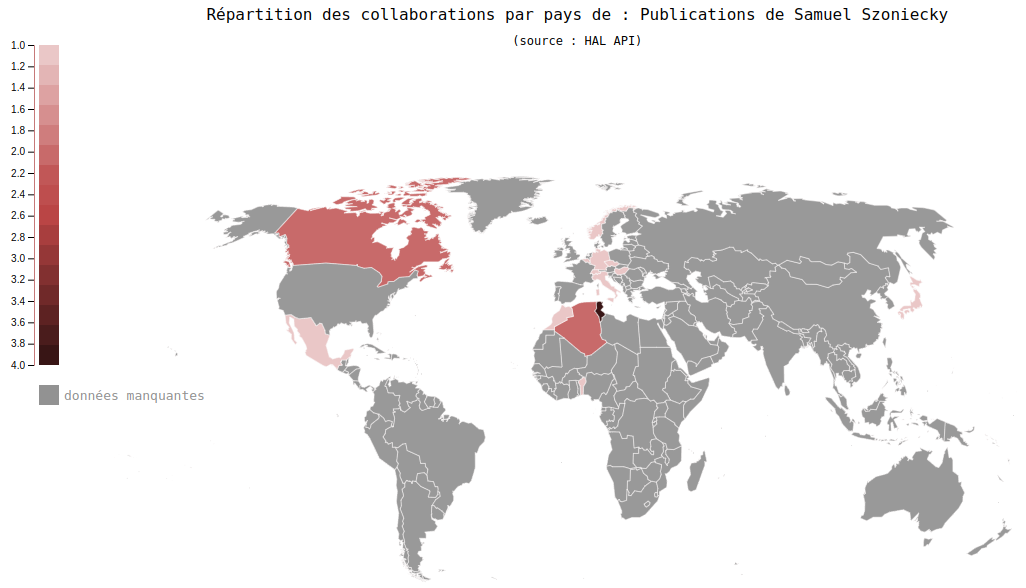
\includegraphics{images/samszo.github.io_StatsHAL_.png}

}

\caption{Répartition des collaborations internationales}

\end{figure}%

\textbf{Mots-clés (domaine de la recherche)} Le diagramme suivant montre
l'évolution des mots-clefs et des collaborations issues de mes
publications dans HAL. Ce diagramme est généré par le dispositif
numérique que nous avons conçu et développé pour analyser les dépôts
dans HAL
cf.~https://samszo.github.io/StatsHAL/?q=authIdHal\_s:samuel-szoniecky

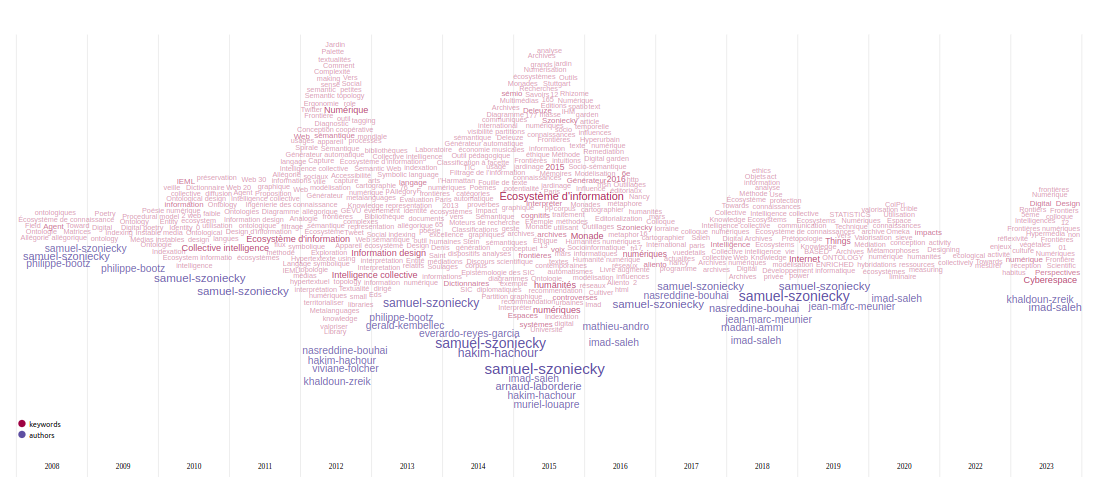
\includegraphics{images/samszo.github.io_StatsHALStream.png}

\textbf{Bibliographie de la synthèse}

\phantomsection\label{refs-synthese}
\begin{CSLReferences}{1}{0}
\bibitem[\citeproctext]{ref-abbott2016}
Abbott, A., Bouvard, H., \& Ollion, É. (2016). L'avenir des sciences
sociales. \emph{Annales. Histoire, Sciences Sociales}, \emph{71e
année}(3), 575--596. Retrieved from
\url{https://www.cairn.info/revue-annales-2016-3-page-575.htm}

\bibitem[\citeproctext]{ref-bachimont2017}
Bachimont, B. (2017). Le numérique comme milieu : enjeux
épistémologiques et phénoménologiques. : Principes pour une science des
données. \emph{Interfaces numériques}, \emph{4}(3), 402--402. Retrieved
from \url{https://www.unilim.fr/interfaces-numeriques/index.php?id=386}

\bibitem[\citeproctext]{ref-berque2009}
Berque, A. (2009). \emph{Ecoumène : Introduction à l'étude des milieux
humains}. Belin.

\bibitem[\citeproctext]{ref-citton2023}
Citton, Y., Lechner, M., \& Masure, A. (2023). \emph{Angles morts du
numérique ubiquitaire}. Presses du réel (Les). Retrieved from
\url{https://journals.openedition.org/lectures/59146}

\bibitem[\citeproctext]{ref-cluxe9ment2021}
Clément, E. (2021). \emph{La flexibilité cognitive: Pierre angulaire de
l'apprentissage}. ISTE éditions.

\bibitem[\citeproctext]{ref-deleuze1988}
Deleuze, G. (1988). \emph{Le pli}. Editions de Minuit.

\bibitem[\citeproctext]{ref-descola2005}
Descola, P. (2005). \emph{Par-delà nature et culture}. Paris: NRF :
Gallimard.

\bibitem[\citeproctext]{ref-desfrichesdoria2022}
Desfriches Doria, O., \& Szoniecky, S. (2022). Les enjeux de la culture
numérique~: des habitus de réception à la réflexivité numérique.
\emph{Approches Théoriques en Information-Communication (ATIC)},
\emph{5}(2), 5--10. Retrieved from
\url{https://www.cairn.info/revue-approches-theoriques-en-information-communication-2022-2-page-5.htm}

\bibitem[\citeproctext]{ref-ertzscheid2023}
Ertzscheid, O. (2023, January 2). GPT-3 : c'est toi le Chat. Retrieved
from
\url{https://affordance.framasoft.org/2023/01/gpt-3-cest-toi-le-chat/}

\bibitem[\citeproctext]{ref-hofstadter2013}
Hofstadter, D., \& Sander, E. (2013). \emph{L'analogie : Coeur de la
pensée}. Odile Jacob.

\bibitem[\citeproctext]{ref-ihadjaduxe8ne2013}
Ihadjadène, M., Szoniecky, S., \& Kembellec, G. (2013).
\emph{Classifications et dispositifs informationnels}. Retrieved from
\url{https://hal-univ-paris8.archives-ouvertes.fr/hal-01098424}

\bibitem[\citeproctext]{ref-laborderie2015}
Laborderie, A., \& Szoniecky, S. (2015). Cultiver son jardin numérique :
métaphore et dispositifs éditoriaux. \emph{Interfaces numériques},
\emph{4}(3), 351--368. Retrieved from
\url{https://hal-bnf.archives-ouvertes.fr/hal-01258307/document}

\bibitem[\citeproctext]{ref-latour2012}
Latour, B. (2012). \emph{Enquêtes sur les modes d'existence : Une
anthropologie des modernes}. Paris: Editions La Découverte.

\bibitem[\citeproctext]{ref-legoux2023}
Legoux, G. (2023, August 1). History of the Generative AI. Retrieved
from
\url{https://medium.com/@glegoux/history-of-the-generative-ai-aa1aa7c63f3c}

\bibitem[\citeproctext]{ref-masure2023}
Masure, A. (2023). \emph{Design sous artifice : la création au risque du
machine learning} (Illustrated édition.). Head Publishing.

\bibitem[\citeproctext]{ref-meunier2018}
Meunier, J.-M., \& Szoniecky, S. (2018). An ontology-based enriched
ebook for teaching statistics. Kyoto, Japan. Retrieved from
\url{https://hal-univ-paris8.archives-ouvertes.fr/hal-01841292}

\bibitem[\citeproctext]{ref-meunier2017}
Meunier, J.-M., Szoniecky, S., \& Lamolle, M. (2017). Colloque
Francophone International sur l{'}Enseignement de la Statistique.
Retrieved from
\url{https://hal-univ-paris8.archives-ouvertes.fr/hal-01565705/document}

\bibitem[\citeproctext]{ref-mineur2022}
Mineur, E. (2022, May 23). Réflexions provisoires liées aux
intelligences artificielles. Retrieved from
\url{https://etienne.design/2022/02/16/ai-3/}

\bibitem[\citeproctext]{ref-saleh2018}
Saleh, I., Ammi, M., \& Szoniecky, S. (2018). \emph{Challenges of the
Internet of Things: Technique, Use, Ethics}. Hoboken, NJ: ISTE Ltd.

\bibitem[\citeproctext]{ref-szoniecky2014}
Szoniecky, S. (2014). ICHSL9 : Alternative Learning Systems. Cotonou,
Bénin. Retrieved from
\url{https://hal-univ-paris8.archives-ouvertes.fr/hal-01098509/document}

\bibitem[\citeproctext]{ref-szoniecky2020}
Szoniecky, S. (2020). Conception d{'}un crible pour mesurer
collectivement les impacts écologiques de l{'}activité. \emph{Les
Cahiers du numerique}, \emph{Vol. 16}(2), 175--199. Retrieved from
\url{https://www.cairn.info/revue-les-cahiers-du-numerique-2020-2-page-175.htm}

\bibitem[\citeproctext]{ref-szoniecky2023}
Szoniecky, S. (2023). Intelligences végétales (pp. 249--255). Presses du
réel (Les). Retrieved from
\url{https://journals.openedition.org/lectures/59146}

\bibitem[\citeproctext]{ref-szoniecky2016}
Szoniecky, S., \& Bouhai, N. (2016). \emph{Collective intelligence and
digital archives}. Hoboken, NJ: ISTE Ltd/John Wiley; Sons Inc.

\bibitem[\citeproctext]{ref-szoniecky2017}
Szoniecky, S., \& Bouhaï, N. (2017). \emph{Intelligence collective et
archives numériques} (Systèmes d'information, web et société.). ISTE
éditions.

\bibitem[\citeproctext]{ref-uxb52015}
µG., Edeline, F., \& Klinkenberg, J.-M. (2015). \emph{Principia
semiotica : Aux sources du sens}. Bruxelles: Les impressions nouvelles
éditions.

\end{CSLReferences}

\section{Activités d'enseignement}\label{activituxe9s-denseignement-1}

\subsection{Jurys}\label{jurys}

\subsubsection{\texorpdfstring{\textbf{Membre de Jury de
Master}}{Membre de Jury de Master}}\label{membre-de-jury-de-master}

En tant que responsable pédagogique j'organise et participe aux jurys de
recrutement et de délivrance des diplômes~:

\begin{itemize}
\item
  Présent - 2018 : Master 2 AVUN
\item
  2019 - 2016 : Licence 3 Pro Design Web Mobile
\item
  2016 - 2010~: Licence 3 Pro Conception Développement Numérique En
  Ligne
\end{itemize}

En tant que membre du département humanités numériques, je participe aux
conseils pédagogique et de perfectionnement pour la mention Humanités
numériques ainsi qu'aux jurys de délivrance de diplôme pour les
formations suivantes~:

\begin{itemize}
\item
  Présent - 2006~: Master 2 Technologie de l'HYPermédia
\item
  Présent - 2014~: Master 2 AVUN
\item
  Présent - 2015~: Master 2 NET
\end{itemize}

J'ai aussi participé de 2009 à 2011 aux jurys de délivrance des
diplômes~du Master EU Management Multimedia 3M2 délivré par le Campus de
la Fonderie de l'image (CNA-CEFAG), Bagnolet~

\subsubsection{\texorpdfstring{\textbf{Membre de Jury de
thèses}}{Membre de Jury de thèses}}\label{sec-juryThese}

\begin{itemize}
\item
  2019 \textbf{\emph{Jury de thèse de El Hadji Malick Gueye}},
  Politiques d'accès aux données statistiques sur le web à l'ère de
  l'open data : pratiques et perspectives. Cas des Instituts Nationaux
  de Statistique d'Afrique membres du réseau AFRISTAT.
\item
  2018 \textbf{\emph{Jury de thèse de The Loc Nguyen}},
  Non-pharmacological interventions : terminology acquisition and
  visualization
\item
  2018 \textbf{\emph{Jury de thèse de Mohamed Benabid}}, Pratiques de
  consommation et processus de changement organisationnel : cas du
  marché de l'information en ligne
\item
  2016 \textbf{\emph{Jury de thèse de Mathieu Andro}}, Bibliothèques
  numériques et crowdsourcing : expérimentations autour de Numalire,
  projet de numérisation à la demande par crowdfunding
\end{itemize}

\subsection{Production de documents
pédagogiques~}\label{production-de-documents-puxe9dagogiques}

Dans le cadre de mon activité d'enseignement je mets à disposition des
étudiants les documents pédagogiques suivants~:

\subsubsection{Supports de cours}\label{supports-de-cours}

Les supports de cours sont disponibles directement sur mon site web sous
la forme de diaporama dynamiques et interactifs, par exemple~:

\begin{itemize}
\item
  \url{https://samszo.github.io/ConfErrance/cours_websemantique/}
\item
  \url{https://samszo.github.io/ConfErrance/cours_semiologie/}
\item
  \url{https://samszo.github.io/ConfErrance/cours_systeme-information-programation-internet/}
\end{itemize}

Pour les étudiants plus curieux, je mets à disposition l'ensemble des
supports de présentation que j'utilise pour mes conférences :
\url{https://samszo.github.io/ConfErrance/}

Les documents pédagogiques pour les cours techniques sont constitués
d'exemples de codes mis à disposition sur la plateforme collaborative
GitHub sous la forme de projet auquel les étudiants participent. Le
tableau ci-dessous a été généré automatiquement avec un outil
d'extraction des données de GitHub :
\url{https://samszo.github.io/HDR/githubStats.html}

Cette plateforme est aussi utilisée par les étudiants pour mettre à
disposition leurs réponses aux exercices demandés, poser leurs
questions, suivre les corrections.~

\begin{longtable}[]{@{}
  >{\raggedright\arraybackslash}p{(\columnwidth - 4\tabcolsep) * \real{0.2000}}
  >{\raggedright\arraybackslash}p{(\columnwidth - 4\tabcolsep) * \real{0.4000}}
  >{\raggedright\arraybackslash}p{(\columnwidth - 4\tabcolsep) * \real{0.4000}}@{}}
\toprule\noalign{}
\begin{minipage}[b]{\linewidth}\raggedright
Année
\end{minipage} & \begin{minipage}[b]{\linewidth}\raggedright
Parcours
\end{minipage} & \begin{minipage}[b]{\linewidth}\raggedright
URL
\end{minipage} \\
\midrule\noalign{}
\endhead
\bottomrule\noalign{}
\endlastfoot
\textbf{2023 - 2022} &
\href{http://localhost/samszo/omk/s/fiches/item/299413}{Master 2 THYP} &
\url{https://github.com/samszo/THYP_22-23} \\
& \href{http://localhost/samszo/omk/s/fiches/item/299414}{Master 2 AVUN}
& \url{https://github.com/samszo/AVUN_22-23} \\
& \href{http://localhost/samszo/omk/s/fiches/item/299420}{Master 2 GSI}
& \url{https://github.com/samszo/M2GSI_22-23} \\
\textbf{2022 - 2021} &
\href{http://localhost/samszo/omk/s/fiches/item/299413}{Master 2 THYP} &
\url{https://github.com/samszo/THYP_21-22} \\
& \href{http://localhost/samszo/omk/s/fiches/item/299414}{Master 2 AVUN}
& \url{https://github.com/samszo/AVUN_21-22} \\
& \href{http://localhost/samszo/omk/s/fiches/item/299420}{Master 2 GSI}
& \url{https://github.com/samszo/M2GSI_21-22} \\
\textbf{2021 - 2020} &
\href{http://localhost/samszo/omk/s/fiches/item/299413}{Master 2 THYP} &
\url{https://github.com/samszo/THYP_20-21} \\
& \href{http://localhost/samszo/omk/s/fiches/item/299414}{Master 2 AVUN}
& \url{https://github.com/samszo/AVUN_20-21} \\
& \href{http://localhost/samszo/omk/s/fiches/item/299420}{Master 2 GSI}
& \url{https://github.com/samszo/M2GSI_20-21_ProgramSystem} \\
& \href{http://localhost/samszo/omk/s/fiches/item/301900}{Master Méga
Données et Analyse Sociale (MéDAS)} &
\url{https://github.com/samszo/MEDAS-1_20-21} \\
& \href{http://localhost/samszo/omk/s/fiches/item/299416}{Master 1 NET}
& \url{https://github.com/samszo/ADLN_20-21} \\
\textbf{2020 - 2019} &
\href{http://localhost/samszo/omk/s/fiches/item/299413}{Master 2 THYP} &
\url{https://github.com/samszo/THYP_19-20} \\
& \href{http://localhost/samszo/omk/s/fiches/item/299414}{Master 2 AVUN}
& \url{https://github.com/samszo/AVUN_19-20} \\
& \href{http://localhost/samszo/omk/s/fiches/item/299421}{Licence Pro
Design Web Mobile} & \url{https://github.com/samszo/DWM_19-20} \\
& \href{http://localhost/samszo/omk/s/fiches/item/301900}{Master Méga
Données et Analyse Sociale (MéDAS)} &
\url{https://github.com/samszo/MEDAS_1_19-20} \\
\textbf{2019 - 2018} &
\href{http://localhost/samszo/omk/s/fiches/item/299413}{Master 2 THYP} &
\url{https://github.com/samszo/THYP_18-19} \\
& \href{http://localhost/samszo/omk/s/fiches/item/299414}{Master 2
AVUN}, \href{http://localhost/samszo/omk/s/fiches/item/299420}{Master 2
GSI} & \url{https://github.com/samszo/GSI-AVUN_18-19} \\
& \href{http://localhost/samszo/omk/s/fiches/item/299421}{Licence Pro
Design Web Mobile} & \url{https://github.com/samszo/DWM_18-19} \\
& \href{http://localhost/samszo/omk/s/fiches/item/299412}{Licence Pro
OCI} & \url{https://github.com/samszo/OCI_18-19} \\
\textbf{2018 - 2017} &
\href{http://localhost/samszo/omk/s/fiches/item/299413}{Master 2 THYP} &
\url{https://github.com/samszo/THYP_17-18} \\
& \href{http://localhost/samszo/omk/s/fiches/item/299414}{Master 2 AVUN}
& \url{https://github.com/samszo/AVUN_17-18} \\
& \href{http://localhost/samszo/omk/s/fiches/item/299412}{Licence Pro
OCI} & \url{https://github.com/samszo/OCI_17-18} \\
\textbf{2017 - 2016} &
\href{http://localhost/samszo/omk/s/fiches/item/299413}{Master 2 THYP} &
\url{https://github.com/samszo/THYP_16-17} \\
& \href{http://localhost/samszo/omk/s/fiches/item/299421}{Licence Pro
Design Web Mobile} & \url{https://github.com/samszo/CDNL_16-17} \\
& \href{http://localhost/samszo/omk/s/fiches/item/299412}{Licence Pro
OCI} & \url{https://github.com/samszo/OCI_16-17} \\
\textbf{2016 - 2015} &
\href{http://localhost/samszo/omk/s/fiches/item/299413}{Master 2 THYP} &
\url{https://github.com/samszo/THYP_15-16} \\
& \href{http://localhost/samszo/omk/s/fiches/item/299421}{Licence Pro
Design Web Mobile} & \url{https://github.com/samszo/CDNL_15-16} \\
& \href{http://localhost/samszo/omk/s/fiches/item/299412}{Licence Pro
OCI} & \url{https://github.com/samszo/oci_15-16} \\
\end{longtable}

\subsubsection{Veille ciblée}\label{veille-cibluxe9e}

Grâce à la plateforme de gestion collaborative de signets Diigo les
étudiants peuvent accéder à une veille ciblée sur un ensemble de notions
en lien avec le cours, par exemple~:

\begin{itemize}
\item
  \href{https://www.diigo.com/user/luckysemiosis?query=\%23th\%C3\%A8se}{Veille
  sur les thèses}
\item
  \href{https://www.diigo.com/user/luckysemiosis?query=\%23THYP}{Veille
  pour le parcours THYP}
\item
  \href{https://www.diigo.com/user/luckysemiosis?query=\%23actulivre}{Veille
  sur la parution d'ouvrages scientifiques}
\end{itemize}

\subsubsection{Bibliographie
commentée}\label{bibliographie-commentuxe9e}

Une bibliographie des ouvrages et articles importants dans le domaine
est accessible en ligne avec des commentaires et des citations~:
\href{https://www.zotero.org/luckysemiosis/items}{\ul{https://www.zotero.org/luckysemiosis/items}}~~

\subsection{Conception de dispositifs pédagogiques
innovants}\label{conception-de-dispositifs-puxe9dagogiques-innovants}

Parallèlement aux documents pédagogiques classiques, j'ai conçu et
développé des dispositifs numériques pour accompagner mes enseignements.

\subsubsection*{2021 - 2022~: Pédagothèque pour l'enseignement de la
psychologie}\label{sec-porjetPedagotheque}
\addcontentsline{toc}{subsubsection}{2021 - 2022~: Pédagothèque pour
l'enseignement de la psychologie}

En partenariat avec l'Université Ouverte des Humanités (UOH)
\url{https://uoh.fr/front/} et en collaboration avec Jean-Marc Meunier,
nous avons développé une pédagothèque pour l'enseignement de la
psychologie \url{https://pedagotheque.uoh.fr/psy/}.

\subsubsection{Module Innovant Pédagogique IDEFI-CreaTIC - EUR
ArTec}\label{module-innovant-puxe9dagogique-idefi-creatic---eur-artec}

Dans le cadre des Initiatives d'Excellence en Formations Innovantes,
j'ai participé depuis sa conception au projet
CréaTIC~(\href{http://idefi-creatic.net/fr/}{\ul{http://idefi-creatic.net/fr/}}\ul{)}~en
proposant des MIP (Modules Innovant Pédagogique). De même, dans le cadre
de l'EUR ou en collaboration avec Philippe Bootz et Ines Laïtano, nous
animons un MIP en littérature numérique.

\begin{longtable}[]{@{}
  >{\raggedright\arraybackslash}p{(\columnwidth - 2\tabcolsep) * \real{0.2000}}
  >{\raggedright\arraybackslash}p{(\columnwidth - 2\tabcolsep) * \real{0.8000}}@{}}
\toprule\noalign{}
\endhead
\bottomrule\noalign{}
\endlastfoot
\textbf{Présent - 2019} & \textbf{\emph{Atelier génération de texte}}

Ce MIP s'inscrit dans le cadre du partenariat international entre ArTeC
et le Rochester Institute of Technology (RIT). L'objectif est de
maîtriser la gestion d'un projet créatif numérique au sein d'une équipe
internationale en mettant en œuvre des méthodologies de communication
numérique collaborative synchrones et asynchrones.

En collaboration avec : Laura Shackelford (RIT), Philippe Bootz
(Paragraphe)

Exemple de réalisation :
\url{https://samszo.github.io/genStory24/?idStory=1} \\
\textbf{2019 - 2018} & \begin{minipage}[t]{\linewidth}\raggedright
\textbf{\emph{Jardiner les écosystèmes de connaissances}}

\emph{En collaboration avec} : Les Archives Nationales de France, Renée
Bourassa (Université Laval, Canada), Chu-Min Chen (INREV, Paris 8),
Everardo Reyes (Paragraphe), Jean-Marc Meunier (Paragraphe),
Marie-Cécile Bouju
(\href{https://idhes.univ-paris8.fr/-idhe-s-}{IDHE.S}), Arnaud
Laborderie (BNF)

\emph{Atelier laboratoire}~: Développer des graines de connaissances

Cet atelier prolonge ceux menés ces dernières années dans le champ de
l'E-éducation (\url{http://gapai.univ-paris8.fr/CreaTIC/E-}
education/Proverbes/, \url{http://gapai.univ-paris8.fr/CreaTIC/CREP/} ),
de la production d'Epub pour l'enseignement des statistiques
(\url{http://www.ontostats.univ-paris8.fr/} ) et de la valorisation des
archives numériques
(\url{http://valarnum.univ-paris8.fr/Atelier-CreaTIC} ). Nous nous
concentrons cette année sur les problématiques de génération automatique
d'interfaces numériques dédiées à la consultation et l'expression de
connaissances via des cartographies sémantiques.

\emph{Séminaire de recherche}~: Vie imaginaire et Intelligence
artificielle

\emph{Hackathon}~: Les Archives Nationales font leur Hackathon
\href{http://www.archives-nationales.culture.gouv.fr/les-archives-nationales-font-leur-hackathon}{\ul{http://www.archives-nationales.culture.gouv.fr/les-archives-nationales-font-leur-hackathon}}

Ce hackathon fait suite à l'atelier laboratoire de 2017-2018 «
Valorisation pédagogique des archives numériques » et au Dev-Camp
organisé par les Archives Nationales en octobre 2017. Il est lié à
l'atelier laboratoire « Graines de connaissances » qui préparera les
étudiants d'un point de vue technique et à l'atelier laboratoire «
Métiers des archives ». Il s'est déroulé le vendredi 16 novembre à 18 h
aux Archives Nationales, site de Paris et portait sur les rapports entre
citoyenneté et archives.

\emph{Workshop}~: Perspectives du livre numériques

Suite aux ateliers « graines de connaissances », « Imaginer le
changement », « Cartographier les pouvoirs d'agir », « animat » et « le
livre augmenté », un jury a sélectionné les meilleures productions
étudiantes pour les inviter à participer à cet événement. Ce workshop a
pour triple ambition de :\\
- partager les bonnes pratiques en matière de conception,
d'éditorialisation, de développement et de diffusion des livres
augmentés\\
- d'expérimenter ces pratiques pour produire des prototypes de livres
augmentés\\
- de consolider les relations scientifiques et pédagogiques entre
CreaTIC, l'Institut Technologies de l'Information et Sociétés, le CRILQ
et le Lantiss\strut
\end{minipage} \\
\textbf{2018 - 2017} & \textbf{\emph{Valorisation des archives
numériques}}

\emph{Atelier laboratoire} : Conception de ressources pédagogiques pour
les archives numériques
\href{https://valarnum.univ-paris8.fr/Atelier-CreaTIC}{\ul{https://valarnum.univ-paris8.fr/Atelier-CreaTIC}}

\emph{Séminaire} : Valorisation pédagogique des archives numériques
\url{https://valarnum.univ-paris8.fr/} \\
\textbf{2017 - 2016} & \textbf{\emph{Créativité, reconstruction,
proverbes}}

\emph{Séminaire}~: Créativité, reconstruction, proverbes, octobre à
décembre 2016, Paris 8

\emph{Atelier laboratoire} : Créativité, reconstruction, proverbes, 17
au 20 janvier 2017, Centre d'art D'Haïti, Port au Prince

\emph{En collaboration avec} : Le centre d'art d'Haïti, Claude Yacoub
(Paragraphe), Stéphane Safin (Paragraphe)

L'atelier consiste à réaliser une action de recherche et formation sur
la créativité dans les territoires désorganisés suite à l'effondrement
des institutions après des catastrophes naturelles et/ou politiques. Le
terrain sur lequel portera l'atelier est Haïti. Cette recherche­action
consiste premièrement à développer et expérimenter de nouveaux outils de
créativité spécifiquement conçus pour impliquer des populations en
situation de reconstruction dans l'expression de leurs besoins matériels
et immatériels, deuxièmement à expérimenter l'usage de la sagesse
populaire, par l'intermédiaire de ses formes courtes que sont les
proverbes, comme source d'inspiration pour la créativité et,
troisièmement, à analyser, comprendre et documenter les activités
créatives mises en oeuvre dans le cadre des ateliers qui seront mis en
place dans les contextes de reconstruction

\href{/annexes/AtelierCReP-Description.pdf}{Description du projet}

\textbf{\emph{Ontologie pour les statistiques}}

\emph{Atelier laboratoire} \textbf{:} Ontologie pour le référencement
des ressources pédagogique en statistiques
\href{https://ontostats.univ-paris8.fr/}{\ul{https://ontostats.univ-paris8.fr/}}

\emph{En collaboration avec} : Jean-Marc Meunier (Paragraphe)

\href{/annexes/e-educationV1.pdf}{Présentation de l'atelier}

\textbf{\emph{Hyperurbains et smartcities}}

\emph{Atelier laboratoire} : Conception de dispositifs numériques pour
le voyage connecté

\emph{En collaboration avec} : Khaldoun Zreik (Paragraphe), Catherine
Nyeki (Artiste numérique)

Dans cet atelier les étudiants ont travaillé sur la réalisation d'un
Alternative Reality Game (ARG). Cette nouvelle forme d'édition numérique
se développe suivant 4 règles fondamentales~: \textbf{\emph{1)
Transmédias :}} l'ARG se développe avec tous les moyens nécessaires et
usuels de la vie courante : affiches, carte à jouer, téléphone,
applications, mails, réseaux sociaux, contact humain\ldots{}

\textbf{\emph{2) Enigmes :}} la progression dans le scénario ludique est
rythmée par différentes tâches à accomplir qui doivent être suffisamment
ardues pour inciter à l'entraide et à l'échange d' information afin de
faire émerger une communauté.

\textbf{\emph{3) Puppet Master :}} Personnage central appelé
«Marionnettiste» qui fait l'interface entre le joueur et histoire. Ce
personnage clé fait donc bien entendu partie du récit.

\textbf{\emph{4) ThisisnotaGame !}} : C'est la devise du jeu en réalité
alternée, faire en sorte que le joueur puisse être en immersion totale,
que le jeu soit une expérience du réel. \\
\textbf{2016 - 2015} & \textbf{\emph{Manuel de créativité}}

\emph{Séminaire} : Outils de créativité pour la reconstruction, 25, 26
juin 2015, Abbaye de Saint Riquier.

\emph{En collaboration avec} : Abbaye de Saint Riquier, Claude Yacoub
(Paragraphe), Stéphane Safin (Paragraphe)

L'atelier consiste à réaliser une recherche/action sur la créativité
dans les territoires désorganisés suite à l'effondrement des
institutions après des catastrophes naturelles et/ou des conflits. En
2016­2017, le terrain choisi est Haïti. Cette recherche­action consiste
d'une part à développer et expérimenter de nouveaux outils de créativité
spécifiquement conçus pour répondre à des demandes particulières des
acteurs de terrain et, d'autre part, à analyser, comprendre et
documenter les activités créatives mises en oeuvre dans le cadre des
ateliers qui seront mis en place dans les contextes de reconstruction.

\href{/annexes/Atelier-LaboratoireCreativiteReconstruction.pdf}{Description
de l'atelier}

\textbf{\emph{Proverbes et e-éducation}}

\emph{Séminaire} : Apprendre par les proverbes, MSH Paris Nord, 26
janvier 2016

\emph{Atelier laboratoire} : Conception de ressources pédagogiques
numériques à partir de proverbes

\emph{En collaboration avec} : Abdenbi Lachkar (Département d'études
arabes, Paris 8), -DIAB-DURANTON Salam Diab-Duranton (Département
d'études arabes, Paris 8)

L'atelier « Proverbes et E-EDUCATION », faisant le lien entre l'étude
des formes de discours courtes et l'interculturalité, consiste à
concevoir un dispositif numérique pour l'E-Education. Le thème abordé en
2015-2016 est l'apprentissage des langues à partir de l'interprétation,
de la traduction et de la sémantisation de proverbes. Les contenus
produits à travers ce dispositif seront utilisés pour expérimenter avec
des lycéens de Saint-Denis l'évaluation des frontières culturelles,
sémantiques et interprétatives.

\href{/annexes/ProverbesEducation2015-2016.pdf}{Bilan de l'atelier}

\textbf{\emph{Hyperurbains et smartcities}}

\emph{Atelier laboratoire} : Conception de dispositifs numériques pour
le voyage connecté

\emph{En collaboration avec} : Khaldoun Zreik (Paragraphe), Catherine
Nyeki (Artiste numérique)

Cet atelier propose d'explorer les nouvelles formes d'informations et de
la communication dans le cadre de la ville connectée. L'atelier s'est
déroulé au premier semestre à Paris 8 dans le cadre d'un cours du Master
2 Net avec une dizaine d'étudiants venant en grande majorité du Master
NET. L'objectif était de concevoir un dispositif numérique pour de
nouveaux usages dans le train et de l'expérimenter sur la ligne Paris
\textless-\textgreater{} Milan.

\href{/annexes/hyperurbainV1.pdf}{Description de l'atelier} \\
\textbf{2015 - 2014} & \textbf{\emph{Le livre post-numérique}}

\emph{Atelier laboratoire} : Le livre post-numérique : création et
édition collaborative scientifique

\emph{Conférence}~: Livre post-numérique : historique, mutations et
perspective, Fès, Maroc

Cet atelier-laboratoire a été conçu dans le cadre du
17\textsuperscript{e} colloque sur le document numérique (CIDE 17)
consacré au «~Livre post-numérique~: historique, mutations et
perspectives~» dont il a constitué le volet expérimental. L'objectif
était de répondre à la problématique du colloque par l'expérimentation
en proposant aux étudiants de concevoir des dispositifs numériques et
créer des prototypes. L'atelier s'est appuyé sur l'expérience du Master
CEN autour des projets éditoriaux et du Master NET autour des ateliers
d'ergonomie, le Master intelligence du Web apportant son orientation
vers les enjeux algorithmiques et humains de l'intelligence collective,
enfin les étudiants du master THYP mettant à disposition leurs
compétences en développement Web.

\href{/annexes/creatic-BilanpedagogiqueAtelierlivrepost-numerique_2015.pdf}{bilan
pédagogique}

\textbf{\emph{Archives en Italie}}

\emph{Atelier laboratoire} : Conception d'une base de donnée pour les
humanités numériques \\
\end{longtable}

\subsection{Encadrement de mémoires de
master}\label{encadrement-de-muxe9moires-de-master}

Dans le cadre des Master du département Humanités numériques j'ai suivie
les travaux d'une trentaine d'étudiants.

\subsubsection{Master 2 NET}\label{master-2-net}

Dans cette formation, les étudiants produisent un mémoire considéré
comme un premier travail de recherche.

2018~- Hadjira Oumennor Makhaldi, À l'ère du numérique~: Comment
pourrait fonctionner l'agriculture du XXIe siècle ?~

2017 - Gabrielle Godin : Théâtre et téléprésence : Enjeux de
communication

2016~- Caroline Avril, Scénographie Émotive~: Interfacer les émotions

2015~- Maxime Antremont, Abstractions numériques : Processus de création
et négociation du sens dans la conception et l'usage d'artefacts
numériques

2014~- Yann Soubai, Espaces associatifs de création et de diffusion
culturelles

\subsubsection{Master 2 THYP}\label{master-2-thyp}

Dans cette formation, les étudiants produisent un rapport de stage.

2016 - Asmae El Miloudi, Développement site web dynamique

2016 - Xiaohe Cao, Développement d'une application HTML5 hors ligne

2015 - Zineb Slaoui, Milliweb

2015 - Karima Hajjari, Développement de modules pour une solution de
place de marché sur internet

2014 - Youcef Chahed, Etudes, Conception et Réalisation d'un Système
Web~

2014 - Firdaous Boumarsel, Rapport de stage de fin d'études ALBIANT-IT
filiale du groupe BPCE

2014 -- Mohame, El Frihmat, Création d'une application de gestion
Participation à la refonte du site web actuel

2013 - Fahem Irantene, Réalisation d'une application centralisant les
multiples opérations des différents départements de l'UPR IDF

2013 - Nadir Gharzal, Participation à la mise en œuvre d'une application
web~: Accueil Client

2013 - Halima Hammouda, Librairie onisep.fr

2012 - Chaimae Alami Mchichi, Stage intégrateur e-CRM et réalisation de
développements sur la plateforme Neolane

2012 - Ala Aldin Atrash, Transforming GEVU Web application to mobile
application using Adobe Flex

2010 - Ahlem Abderrahmane, Rapport de stage, CapSanté

2010 - Mehdi Touibi, Implémentation d'une application web 2.0 pour
l'évaluation de l'activité politique des députés français au sein de
l'Assemblée Nationale

2009 - Bachar ALBOUZ, Rapport de stage Direct interactiv

2009 -~ Bachir Bouslougui, Navigateur Spatio-temporel

2009 - Bargaoui Abderrahim, Plugin Firefox pour l'archivage de la poésie
numérique

2008 - Olloi Dede, Réalisation d'un monitoring des activités
d'Outsourcing

2008 - Aquil Ramzan, Développement d'un EDI éditeur et d'un guide
shopping

2007 - Rime Karout, Création de la deuxième version du CMS EasyPlay

2007 - Karim Elhousny, Euro-Méditérranée Tours, Rapport de stage

2007 - Ahmed Mohamed, Evolution du système d'information du musée du
sport

2007 - Hassen Boumaraf, Mise en place d'un intranet d'entreprise

2006 - Mehdi Benzarti, Modélisation et conception d'une base de données
et création des interfaces de saisies pour l'étude P2M

2006 - Karima Kadri, Création d'un système d'information pour le
contrôle de gestion aux Galeries Lafayette

\subsubsection{Master 2 Ergonomie}\label{master-2-ergonomie}

Dans cette formation, les étudiants produisent un mémoire considéré
comme un premier travail de recherche.

2017 - Eléonore Gouttegata, L'ergonomie au service de la conception~: un
outil numérique pour favoriser la recherche en sciences humaines et
sociales

\subsection{Présentation des principaux
enseignements}\label{pruxe9sentation-des-principaux-enseignements}

Les cours que je donne depuis 2005 se font essentiellement à
l'université Paris 8 dans le département Humanité numériques,
anciennement Hypermédia, ce sont des cours en présentiels sauf depuis la
pandémie de Covid où suivant la situation sanitaire je donne des cours à
distance par visioconférence. Ce sont principalement des cours de
Licence 3 professionnelle et de Master 1 et 2 qui s'adressent à un
public en formation initiale venant de parcours très différents~:
information communication, informatique, sciences humaines, journalisme,
graphisme\ldots{}

L'objectif pédagogique principal consiste à montrer que dans les métiers
du numérique ces disciplines sont complémentaires et que leurs mise en
pratique dans des projets en équipe permet de s'enrichir des compétences
des uns et des autres. J'insiste beaucoup sur la nécessité de développer
tout à la fois des compétences techniques, des points de vue théoriques
et des pratiques collaboratives efficaces. Il me semble aussi très
important de transmettre aux étudiants l'idée que l'apprentissage est
une pratique continue surtout dans une domaine très évolutif comme celui
du numérique et que les cours sont que les prémices d'un formation tout
au long de la vie.

Parallèlement à mes cours de Paris 8, tous les ans je donne un ou deux
cours dans des établissements publics afin de m'enrichir d'ambiances, de
pratiques et de public différents.

\subsubsection{\texorpdfstring{\textbf{Département Humanités Numériques
-- Université Paris
8}}{Département Humanités Numériques -- Université Paris 8}}\label{duxe9partement-humanituxe9s-numuxe9riques-universituxe9-paris-8}

\begin{longtable}[]{@{}
  >{\raggedright\arraybackslash}p{(\columnwidth - 4\tabcolsep) * \real{0.3000}}
  >{\raggedright\arraybackslash}p{(\columnwidth - 4\tabcolsep) * \real{0.2000}}
  >{\raggedright\arraybackslash}p{(\columnwidth - 4\tabcolsep) * \real{0.5000}}@{}}
\toprule\noalign{}
\begin{minipage}[b]{\linewidth}\raggedright
Parcours
\end{minipage} & \begin{minipage}[b]{\linewidth}\raggedright
Années
\end{minipage} & \begin{minipage}[b]{\linewidth}\raggedright
Cours
\end{minipage} \\
\midrule\noalign{}
\endhead
\bottomrule\noalign{}
\endlastfoot
Master CEN (Création Edition Numérique)

\url{https://humanites-numeriques.univ-paris8.fr/-Masters-CEN-} &
Présent - 2020 & \textbf{\emph{Approches transversales des humanités
numériques (6H)}}

Présentation des enjeux techniques et scientifiques des Humanités
Numériques. \\
& & \textbf{\emph{Participation critique (30H)}}

Ce cours intensive réuni pendant une semaine les étudiants de la Mention
Humanité numérique pour après à deux jours de présentations
d'universitaires et de professionnels sur un thème, concevoir une note
d'intention sur un dispositif numérique mettant en pratique le thème
abordé. \\
& 2016 - 2015 & \textbf{Javascript pratique} (20H)

Mise en pratique du Javascript par une pédagogie par projet \\
& 2015 - 2013 & \textbf{Atelier 3D} (40H)

Cours intensif pour la conception, la réalisation et la diffusion d'un
dispositif Web 3D. \\
& 2010 - 2009 & Technique du Web : XML (40H)

Cours intensif pour la conception, la réalisation et la diffusion d'un
dispositif Web 3D. \\
& & \textbf{Accessibilité Web, internet, multi modalité, communication
homme/machine} (40H)

Cours pour former les étudiants à la maîtrise des flux d'information et
de communication dans un environnement Web \\
Master 2 THYP (Technologie de l'HYPermédia)

\url{https://www.univ-paris8.fr/-Master-Technologies-de-l-Hypermedia-678-}
& Présent - 2012 & \textbf{Langages du Web} (40H)

Explication des théories et mise en pratique des langages du WEB~: html,
javascript, Zend Framework, SVG, XML\ldots{} \\
Master 2 AVUN (Analyse et Valorisation des Usages Numériques) jusqu'en
2022 puis Master 2 ACEHN (Analyses et Conception de Environnements
Humains Numériques )

\url{https://humanites-numeriques.univ-paris8.fr/-Master-ACEHN-} &
Présent - 2014 & \textbf{Ethique du web et écosystèmes d'information}
(30H)

Cours pour sensibiliser les étudiants à la complexité de
l'information-communication par une modélisation écosystémique suivant
une problématique éthique. \\
Master 2 GSI (Gestion Stratégique de l'Information)

\url{https://humanites-numeriques.univ-paris8.fr/-Master-G-S-I-} &
Présent - 2020 & \textbf{\emph{Systèmes d'information et programmation
Internet}}

\emph{Description} : Cours pour comprendre en quoi un système
d'information est un écosystème et comment le développer en utilisant
des langages de programmation Web. \\
Licence de Psychologie IED

\url{https://www.iedparis8.net/?-licence-de-psychologie-} & Présent -
2019 & \textbf{\emph{Méthodologie de travail collaboratif (50H)}}

L'objectif de ce cours est de développer des compétences transversales
en vous formant au travail collaboratif en ligne. Nous vous donnerons
dans ce cours des outils d'autoévaluation de vos compétences, vous
formerons à l'utilisation d'outils collaboratifs en ligne et vous ferons
travailler un groupe pour réaliser un projet. \\
Master 2 NET (Numérique : Enjeux, Technologies)

\url{https://humanites-numeriques.univ-paris8.fr/-N-E-T-} & 2017 - 2015
& \textbf{Hyperurbain} (30H)

Cours pour la conception collaborative de dispositifs numériques
innovant dans le cadre de la ville connecté. \\
Licence Pro DWM (Design Web Mobile) anciennement CDNL (Création
Développement Numérique en Ligne) & 2019 - 2010 & \textbf{Rencontres
média} (60H)

L'objectif de ce cours consiste à proposer à des étudiants en
apprentissage, une vision théorique de leurs métiers par la rencontre
avec des acteurs universitaires dans leur domaine. Savoir identifier les
fondamentaux de la création numérique, analyse, synthèse. Élaborer et
argumenter de manière critique des modèles théoriques et des
recommandations pratiques. Analyser des contenus hypermédia (texte,
image, son et vidéo). \\
& 2019 - 2013 & \textbf{Réalisation avancée en développement} (40H)

Ce cours présente les technologies pour concevoir et réaliser des
dispositifs numériques en ligne, par exemple modéliser et intégrer des
bases de données en appliquant une méthode de conception, connaître et
savoir appliquer les règles d'accessibilité pour des pages Web, prendre
en compte les balises sémantiques et les micro formats. \\
& & \textbf{Perfectionnement outils et langages de base} (40H)
\textbar{} \textbar{} Ce cours forme les étudiants aux compétences
suivantes~: \textbar{} \textbar{} - Gérer des formats, créer et produire
de l'iconographie, traiter les images. \textbar{} \textbar{} - Connaître
les techniques de numérisation, d'optimisation de poids et de
compression liés à la création, le traitement, la diffusion on/off line
et l'archivage de l'image (2D fixe ou animée), du son et de la vidéo.
\textbar{} \textbar{} - Rédiger des concepts créatifs en fonction du
support choisi (presse, multimédia, spots, radio, TV, affiches, jeux
vidéo, \ldots) \\
& & \textbf{Atelier de projet collaboratif} (40H)

Dans ce cours nous accompagnement les étudiants dans la conception et la
réalisation d'un projet numérique incluant~: une note d'intention, un
teaser vidéo, un site Web, une application mobile et un dossier de
conception. Les étudiants devront rédiger un cahier des charges pour un
projet hypermédia/TIC, savoir communiquer et collaborer avec les équipes
de création et de développement, participer à la réalisation de projets
innovants, mettre en œuvre ou appliquer une méthode de développement
adaptée à un travail d'équipe, savoir réaliser une maquette
fonctionnelle, argumenter et défendre un point de vue en réunion
d'équipe, devant des clients, décideurs, etc. \\
DU Assistant en technologies numériques audiovisuelles & 2015 - 2010 &
\textbf{Conception de site Web} (30H)

Cours pour la conception collaborative d'édition numériques à partir de
CMS et avec les technologie HTML, CSS, javascript. \\
\end{longtable}

\subsubsection{\texorpdfstring{\textbf{Département Informatique --
Université Paris
8}}{Département Informatique -- Université Paris 8}}\label{duxe9partement-informatique-universituxe9-paris-8}

\begin{longtable}[]{@{}
  >{\raggedright\arraybackslash}p{(\columnwidth - 4\tabcolsep) * \real{0.3000}}
  >{\raggedright\arraybackslash}p{(\columnwidth - 4\tabcolsep) * \real{0.2000}}
  >{\raggedright\arraybackslash}p{(\columnwidth - 4\tabcolsep) * \real{0.5000}}@{}}
\toprule\noalign{}
\begin{minipage}[b]{\linewidth}\raggedright
Parcours
\end{minipage} & \begin{minipage}[b]{\linewidth}\raggedright
Années
\end{minipage} & \begin{minipage}[b]{\linewidth}\raggedright
Cours
\end{minipage} \\
\midrule\noalign{}
\endhead
\bottomrule\noalign{}
\endlastfoot
Licence Pro OCI (Objets Communicants Intelligents) & 2020 - 2013 &
\textbf{Gestion de projet} (30H)

Ce cours prépare les étudiants à mieux gérer leurs projets par la mise
en pratique de méthode et d'outils~: Gantt, planning partagé,
gestionnaire de code\ldots{} \\
\end{longtable}

\subsubsection{\texorpdfstring{\textbf{CNAM --
Bretagne}}{CNAM -- Bretagne}}\label{cnam-bretagne}

\begin{longtable}[]{@{}
  >{\raggedright\arraybackslash}p{(\columnwidth - 4\tabcolsep) * \real{0.3000}}
  >{\raggedright\arraybackslash}p{(\columnwidth - 4\tabcolsep) * \real{0.2000}}
  >{\raggedright\arraybackslash}p{(\columnwidth - 4\tabcolsep) * \real{0.5000}}@{}}
\toprule\noalign{}
\begin{minipage}[b]{\linewidth}\raggedright
Parcours
\end{minipage} & \begin{minipage}[b]{\linewidth}\raggedright
Années
\end{minipage} & \begin{minipage}[b]{\linewidth}\raggedright
Cours
\end{minipage} \\
\midrule\noalign{}
\endhead
\bottomrule\noalign{}
\endlastfoot
Certificat de spécialisation CS 61 : Innovations territoriales,
Politiques numériques et Open Data

\url{https://formation.cnam.fr/rechercher-par-discipline/certificat-de-specialisation-innovations-territoriales-politiques-numeriques-et-open-data-777352.kjsp}
& Présent - 2017 & \textbf{Web sémantique pour chef de projet} (6H)

L'objectif de ce cours à distance est de familiariser les étudiants au
technologies du Web sémantique pour qu'ils puissent les appliquer dans
le contexte de leur travail de chef de projet. \\
\end{longtable}

\subsubsection{\texorpdfstring{\textbf{Département Information
Communication -- IUT Paris
Descartes}}{Département Information Communication -- IUT Paris Descartes}}\label{duxe9partement-information-communication-iut-paris-descartes}

\begin{longtable}[]{@{}
  >{\raggedright\arraybackslash}p{(\columnwidth - 4\tabcolsep) * \real{0.3000}}
  >{\raggedright\arraybackslash}p{(\columnwidth - 4\tabcolsep) * \real{0.2000}}
  >{\raggedright\arraybackslash}p{(\columnwidth - 4\tabcolsep) * \real{0.5000}}@{}}
\toprule\noalign{}
\begin{minipage}[b]{\linewidth}\raggedright
Parcours
\end{minipage} & \begin{minipage}[b]{\linewidth}\raggedright
Années
\end{minipage} & \begin{minipage}[b]{\linewidth}\raggedright
Cours
\end{minipage} \\
\midrule\noalign{}
\endhead
\bottomrule\noalign{}
\endlastfoot
DU : Analyse Data science

\url{https://iutparis-seine.u-paris.fr/metiers-de-la-data/diplome-duniversite-analyste-data-science/}
& Présent - 2015 & \textbf{Data visualisation} (4H)

Cours pour la conception de visualisation interactives et dynamiques à
partir de données provenant de l'Open Data. \\
Licence Pro Métiers de la communication : chef de projet communication &
2018 - 2017 & \textbf{Sémiologie} (24H)

Ce cours permet aux étudiants de découvrir les principes fondamentaux de
la sémiologie et des les appliquer dans des cas pratiques. \\
\end{longtable}

\subsubsection{\texorpdfstring{\textbf{Département Communication et
Formation interculturelles -
INALCO}}{Département Communication et Formation interculturelles - INALCO}}\label{duxe9partement-communication-et-formation-interculturelles---inalco}

\begin{longtable}[]{@{}
  >{\raggedright\arraybackslash}p{(\columnwidth - 4\tabcolsep) * \real{0.2000}}
  >{\raggedright\arraybackslash}p{(\columnwidth - 4\tabcolsep) * \real{0.1000}}
  >{\raggedright\arraybackslash}p{(\columnwidth - 4\tabcolsep) * \real{0.7000}}@{}}
\toprule\noalign{}
\begin{minipage}[b]{\linewidth}\raggedright
Parcours
\end{minipage} & \begin{minipage}[b]{\linewidth}\raggedright
Années
\end{minipage} & \begin{minipage}[b]{\linewidth}\raggedright
Cours
\end{minipage} \\
\midrule\noalign{}
\endhead
\bottomrule\noalign{}
\endlastfoot
Master CFI (Communication et Formation interculturelles)

\href{http://www.inalco.fr/departement/communication-formation-interculturelles}{\ul{http://www.inalco.fr/departement/communication-formation-interculturelles}}
& 2017 - 2015 & \textbf{Conception de site Web} (30H)

Ce cours permet aux étudiants de découvrir les langages de base du Web
(HTML, CSS, Javascript) et de développer un premier site en utilisant un
CMS (SPIP, Wordpress) \\
\end{longtable}

\subsubsection{\texorpdfstring{\textbf{Département Science de
L'information et de la Communication - Paris
13}}{Département Science de L'information et de la Communication - Paris 13}}\label{duxe9partement-science-de-linformation-et-de-la-communication---paris-13}

\begin{longtable}[]{@{}
  >{\raggedright\arraybackslash}p{(\columnwidth - 4\tabcolsep) * \real{0.3000}}
  >{\raggedright\arraybackslash}p{(\columnwidth - 4\tabcolsep) * \real{0.2000}}
  >{\raggedright\arraybackslash}p{(\columnwidth - 4\tabcolsep) * \real{0.5000}}@{}}
\toprule\noalign{}
\begin{minipage}[b]{\linewidth}\raggedright
Parcours
\end{minipage} & \begin{minipage}[b]{\linewidth}\raggedright
Années
\end{minipage} & \begin{minipage}[b]{\linewidth}\raggedright
Cours
\end{minipage} \\
\midrule\noalign{}
\endhead
\bottomrule\noalign{}
\endlastfoot
Master DIMI (Design d'interface multimédia et internet) & 2015 - 2012 &
\textbf{Algorithmique} (30H)

Ce cours permet aux étudiants de découvrir les règles de base de
l'algorithmique et de développer un premier programme en Javascript \\
\end{longtable}

\subsubsection{UFR Lettres et Sciences Humaines - Université de Rouen
Normandie}\label{sec-item541157}

\begin{longtable}[]{@{}
  >{\raggedright\arraybackslash}p{(\columnwidth - 4\tabcolsep) * \real{0.3000}}
  >{\raggedright\arraybackslash}p{(\columnwidth - 4\tabcolsep) * \real{0.2000}}
  >{\raggedright\arraybackslash}p{(\columnwidth - 4\tabcolsep) * \real{0.5000}}@{}}
\toprule\noalign{}
\begin{minipage}[b]{\linewidth}\raggedright
Parcours
\end{minipage} & \begin{minipage}[b]{\linewidth}\raggedright
Années
\end{minipage} & \begin{minipage}[b]{\linewidth}\raggedright
Cours
\end{minipage} \\
\midrule\noalign{}
\endhead
\bottomrule\noalign{}
\endlastfoot
Master Humanité Numérique & 2023 - 2022 & \textbf{\emph{Anthropologie et
épistémologie du numérique (30H)}}

Dans ce séminaire, nous explorerons l'écosystème du numérique suivant
deux approches complémentaires, une centrée sur l'humain (Descola) dans
les milieux (Berque) numériques et l'autre sur les connaissances
(Deleuze \& Guattari) produites dans cet écosystème. Ces explorations
seront modélisées sous la forme d'existences informationnelles (Morin,
Latour) dont nous analyserons les pouvoirs de discerner, d'élaborer et
d'agir (Groupe µ). L'objectif principal de ce séminaire est de fournir
aux étudiants une méthode générique pour l'analyse des écosystèmes
(Szoniecky) et l'expression d'un point de vue éthique (Deleuze). \\
\end{longtable}

\section{Activités de recherche}\label{activituxe9s-de-recherche}

\subsection{Encadrement de chercheurs⋅euses}\label{sec-item299365}

\subsubsection*{Thèses soutenues : Co- direction ou co-encadrement de
thèse : quotité
50\%}\label{thuxe8ses-soutenues-co--direction-ou-co-encadrement-de-thuxe8se-quotituxe9-50}
\addcontentsline{toc}{subsubsection}{Thèses soutenues : Co- direction ou
co-encadrement de thèse : quotité 50\%}

\begin{longtable}[]{@{}
  >{\raggedright\arraybackslash}p{(\columnwidth - 2\tabcolsep) * \real{0.0982}}
  >{\raggedright\arraybackslash}p{(\columnwidth - 2\tabcolsep) * \real{0.9018}}@{}}
\toprule\noalign{}
\endhead
\bottomrule\noalign{}
\endlastfoot
Décembre 2016 & \textbf{Mathieu Andro}

\emph{Titre} : Bibliothèques numériques et crowdsourcing :
expérimentations autour de Numalire, projet de numérisation à la demande
par crowdfunding.

\emph{Financement pendant la thèse} : autofinancé

\emph{Situation après la thèse} : Ingénieur text mining à l'Institut
National de la Recherche Agronomique. \\
\end{longtable}

\subsubsection*{Thèses en cours de finalisation : Co- direction de thèse
: quotité
50\%}\label{thuxe8ses-en-cours-de-finalisation-co--direction-de-thuxe8se-quotituxe9-50}
\addcontentsline{toc}{subsubsection}{Thèses en cours de finalisation :
Co- direction de thèse : quotité 50\%}

\begin{longtable}[]{@{}
  >{\raggedright\arraybackslash}p{(\columnwidth - 2\tabcolsep) * \real{0.2081}}
  >{\raggedright\arraybackslash}p{(\columnwidth - 2\tabcolsep) * \real{0.7919}}@{}}
\toprule\noalign{}
\endhead
\bottomrule\noalign{}
\endlastfoot
2018

(prévisionnel de soutenance) & \textbf{Gabrielle Godin}

\emph{Titre (indicatif)} : Ecosystème des ``feuillets numériques'' :
éditorialisation numérique dans le spectacle vivant..

\emph{Financement de la thèse} : Chargée de cours, ingénieure de
recherche. \\
2017

(prévisionnel de soutenance) & \textbf{Amri Toumia}

\emph{Titre (indicatif)} : Protection des données de la vie privée dans
l'Internet des Objets.

\emph{Financement de la thèse} : autofinancé.

\emph{Situation active \& professionnelle} : Ingénieur informatique pour
des start-up. \\
\end{longtable}

\subsubsection{Animation d'une équipe}\label{sec-item299366}

Dans le cadre de la collection d'ouvrage Digital Tools \& Uses, je
participe à l'animation de l'équipe d'auteurs, à la création du site
Web, à l'organisation des conférences\ldots{}
cf.~\url{http://digitaluses.info/}

\subsubsection{Création d'un axe scientifique}\label{sec-item299364}

Dans le cadre de la refonte des équipes du laboratoire Paragraphe, j'ai
participé à la création de l'axe « Dispositifs numériques : production,
usages et modélisation communicationnelle », travaille à son
développement et anime ses activités.

\subsubsection{Comité de suivi de thèse}\label{sec-item299642}

\begin{longtable}[]{@{}
  >{\raggedright\arraybackslash}p{(\columnwidth - 2\tabcolsep) * \real{0.2361}}
  >{\raggedright\arraybackslash}p{(\columnwidth - 2\tabcolsep) * \real{0.7639}}@{}}
\toprule\noalign{}
\endhead
\bottomrule\noalign{}
\endlastfoot
2023 & \begin{minipage}[t]{\linewidth}\raggedright
\begin{itemize}
\item
  Pierre Mickaël Micaletti, Laboratoire Paragraphe
\item
  Shumin Liang, Laboratoire Paragraphe
\item
  Andrea Sosa, Laboratoire Paragraphe
\item
  Mohammed Ahmed Hassan, Laboratoire Paragraphe
\item
  Emna Louati, Laboratoire IREMUS
\end{itemize}
\end{minipage} \\
2022 & \begin{minipage}[t]{\linewidth}\raggedright
\begin{itemize}
\item
  Pierre Manon Micaletti, Laboratoire Paragraphe
\item
  Sarah Malaeb, Laboratoire Paragraphe
\item
  Emna Louati, Laboratoire IREMUS
\end{itemize}
\end{minipage} \\
2021 & \begin{minipage}[t]{\linewidth}\raggedright
\begin{itemize}
\item
  Luis Torres, Laboratoire Paragraphe
\item
  Emna Louati, Laboratoire IREMUS
\end{itemize}
\end{minipage} \\
2020 & \begin{minipage}[t]{\linewidth}\raggedright
\begin{itemize}
\tightlist
\item
  Emna Louati, Laboratoire IREMUS
\end{itemize}
\end{minipage} \\
2019 & \begin{minipage}[t]{\linewidth}\raggedright
\begin{itemize}
\tightlist
\item
  Emna Louati, Laboratoire IREMUS
\end{itemize}
\end{minipage} \\
2018 & \begin{minipage}[t]{\linewidth}\raggedright
\begin{itemize}
\item
  Emna Louati, Laboratoire IREMUS
\item
  Carole Henri, Laboratoire Paragraphe
\end{itemize}
\end{minipage} \\
\end{longtable}

\subsubsection{Encadrement de stagiaire dans le laboratoire
Paragraphe}\label{encadrement-de-stagiaire-dans-le-laboratoire-paragraphe}

\begin{longtable}[]{@{}
  >{\raggedright\arraybackslash}p{(\columnwidth - 2\tabcolsep) * \real{0.2000}}
  >{\raggedright\arraybackslash}p{(\columnwidth - 2\tabcolsep) * \real{0.8000}}@{}}
\toprule\noalign{}
\endhead
\bottomrule\noalign{}
\endlastfoot
2023 & \textbf{Stage de Rim Kaidi}

\emph{Description} : Design d'information pour le bilan du laboratoire
Paragraphe \textbar{}

\emph{Travail pour} : \url{https://github.com/samszo/StatsHAL}
\textbar{} \\
2023 & \textbf{Stage de Christina Ramaroson}

\emph{Description} : Recensement des dispositifs numériques de lutte
contre les fakes news (jeux sérieux, sites de Hoax, fact checking etc.),
élaboration d'un protocole d'expérimentation des dispositifs,
expérimentation et analyse des dispositifs, synthèse. \textbar{}

\emph{Travail pour} :
\href{http://localhost/samszo/omk/s/fiches/item/299716}{polemika}
\textbar{}

\emph{Participant} :
\href{http://localhost/samszo/omk/s/fiches/item/62137}{Orélie Desfriches
Doria} \textbar{} \\
2021 & \textbf{Stage de Chacha Mahfoud}

\emph{Description} : Recherche documentaires structurées, lecture
d'articles scientifiques, rédaction d'un état de l'art sur les fake news
d'après la littérature scientifique, participation aux réunions et
séminaires. \textbar{}

\emph{Travail pour} :
\href{http://localhost/samszo/omk/s/fiches/item/299716}{polemika}
\textbar{}

\emph{Participant} :
\href{http://localhost/samszo/omk/s/fiches/item/62137}{Orélie Desfriches
Doria} \textbar{} \\
2019 & \textbf{Stage de Lucien Cartier-Tilet}

\emph{Description} : Tests et corrections d'un module Omeka S pour le
scraping des textes de Molière. \textbar{}

\emph{Travail pour} :
\href{http://localhost/samszo/omk/s/fiches/item/299592}{EUR ArTeC}
\href{http://localhost/samszo/omk/s/fiches/item/299717}{Omeka-S-module-Scraping}
\textbar{} \\
2018 & \textbf{Stage de Roch Delanay}

\emph{Description} : Conception et développement d'une application de
mailing pour la gestion des publication scientifiques. \textbar{} \\
2012 & \textbf{Stage de Ala Atrash}

\emph{Description} : Conception et développement de la version tactile
de GEVU \textbar{} \\
2012 & \textbf{Stage de Claire Dezaille}

\emph{Description} : Conception de statistiques pour GEVU \textbar{} \\
\end{longtable}

\subsection{Participation à des activités
d'expertise}\label{participation-a-des-activites-dexpertise}

\begin{longtable}[]{@{}
  >{\raggedright\arraybackslash}p{(\columnwidth - 2\tabcolsep) * \real{0.2000}}
  >{\raggedright\arraybackslash}p{(\columnwidth - 2\tabcolsep) * \real{0.8000}}@{}}
\toprule\noalign{}
\endhead
\bottomrule\noalign{}
\endlastfoot
\textbf{2021 - 2020} & \textbf{Soutien à la recherche-création pour la
relève professorale}, Canada. Décembre 2016, Digital Humanities 2017,
Montreal, Canada \\
\textbf{2017 - 2016} & \textbf{Digital Humanities 2017}

\emph{Site Web en relation :} https://dh2017.adho.org/ \\
\textbf{2016} & \textbf{Colloque jeunes chercheurs de l'école doctorale
CLI} : Cognition, Langage, Interaction, Université Paris 8

\emph{Site Web en relation :} http://cli2016.fr/comites.php \\
& \textbf{AAP Interdisciplinaires Phase 2}, Université de Nantes \\
\textbf{2015} & \textbf{Digital Humanities 2016}

\emph{Site Web en relation :} http://dh2016.adho.org/ \\
& \textbf{Colloque jeunes chercheurs de l'école doctorale CLI} :
Cognition, Langage, Interaction, Université Paris 8.

\emph{Site Web en relation :} http://cli2016.fr/comites.php \\
\textbf{2010} & \textbf{ANR Programme CONTENUS ET INTERACTIONS} \\
\end{longtable}

\subsection{Participation à des comités de lecture, éditoriaux et
scientifiques}\label{participation-uxe0-des-comituxe9s-de-lecture-uxe9ditoriaux-et-scientifiques}

\begin{longtable}[]{@{}
  >{\raggedright\arraybackslash}p{(\columnwidth - 2\tabcolsep) * \real{0.2000}}
  >{\raggedright\arraybackslash}p{(\columnwidth - 2\tabcolsep) * \real{0.8000}}@{}}
\toprule\noalign{}
\endhead
\bottomrule\noalign{}
\endlastfoot
\textbf{Présent - 2015} & \textbf{Membre du comité scientifique de la
revue Internet des Objets} dans ISTE Open Science

\emph{Site Web en relation :}
http://www.openscience.fr/Internet-des-objets \\
& \textbf{Membre du comité de la collections « Outils et usages
numériques »}

Cette collection d'ouvrage dirigée par Imad Saleh regroupe uen vingtaine
de chercheurs qui travaillent sur les outils et les usages du numériques

\emph{Site Web en relation :} http://digitaluses.info/ \\
\textbf{Présent - 2017} & \textbf{Membre du comité éditorial de la Revue
sur les langues de moindre diffusion}

Cette revue dirigée par Abderrezak Dourari traite des enjeux des langues
de mondre diffusion notamment concernant les impacts du numérique.

\emph{Site Web en relation :}
https://www.cnplet.dz/component/k2/item/313 \\
\end{longtable}

\subsection{Organisation de séminaires, congrès et colloques de portée
nationale et
internationale}\label{organisation-de-suxe9minaires-congruxe8s-et-colloques-de-portuxe9e-nationale-et-internationale}

\subsubsection{Création d'un colloque international
IEEE}\label{cruxe9ation-dun-colloque-international-ieee}

\begin{longtable}[]{@{}
  >{\raggedright\arraybackslash}p{(\columnwidth - 2\tabcolsep) * \real{0.2000}}
  >{\raggedright\arraybackslash}p{(\columnwidth - 2\tabcolsep) * \real{0.8000}}@{}}
\toprule\noalign{}
\endhead
\bottomrule\noalign{}
\endlastfoot
\textbf{2020} & \textbf{Digital Tools \& Uses -- Congress}

Hammamet - 15, 16 and 17 October 2020,~
https://digitaluses-congress.univ-paris8.fr/ \\
\textbf{2018} & \textbf{Digital Tools \& Uses -- Congress}

Paris - 3, 4 and 5 Octobre 2018,
https://digitaluses-congress.univ-paris8.fr/?page=Paris-2018 \\
\end{longtable}

\subsubsection{Membre d'un comité d'événement
scientifiques}\label{membre-dun-comituxe9-duxe9vuxe9nement-scientifiques}

\begin{longtable}[]{@{}
  >{\raggedright\arraybackslash}p{(\columnwidth - 2\tabcolsep) * \real{0.2000}}
  >{\raggedright\arraybackslash}p{(\columnwidth - 2\tabcolsep) * \real{0.8000}}@{}}
\toprule\noalign{}
\endhead
\bottomrule\noalign{}
\endlastfoot
\textbf{2023} & \textbf{H2PTM 2023}

La fabrique du sens à l'ère de l'information numérique : enjeux et défis
Localisation : Arenberg Creative Mine, Valenciennes, France

\emph{Site Web en relation :} http://h2ptm.univ-paris8.fr/ \\
\textbf{2022} & \textbf{Colloque international - Existences collectives}

Perspectives sémiotiques sur la sociabilité animale et humaine

20-21 octobre 2022, Université Paris 8 et Campus Condorcet

\emph{Site Web en relation :}
\url{https://existencesco.sciencesconf.org/} \\
& \textbf{01 Design 12}

Design Non-intentionel 13, 14 et 15 octobre 2022, Kerkennah Islands,
Tunisia.

\emph{Site Web en relation :} http://01design.eu/12/ \\
\textbf{2021} & \textbf{H2PTM 2021}

Enjeux et nouveaux défis Localisation : Campus Condorcet
Aubervilliers \\
\textbf{2019} & \textbf{H2PTM 2019}

De l'hypertexte aux humanités numériques 16, 17 et 18 octobre 2019,
Université de Franche-Comté, Montbéliard

\emph{Site Web en relation :}
http://h2ptm.univ-paris8.fr/OLD/h2ptm19/ \\
& \textbf{Colloque Le corpus audiovisuel : Quelles approches ? Quels
usages ?}

15 avril 2019, INALCO

\emph{Site Web en relation :} https://calenda.org/584811 \\
\textbf{2018} & \textbf{01Design 11}

Concevoir à l'ère post-numérique, 5-7 Juin, 2018, Maison du Design,
Mons, Belgique

\emph{Site Web en relation :} https://01design.eu/11/ \\
\textbf{2017} & \textbf{H2PTM 2017}

Le numérique à l'ère des designs : de l'hypertexte à l'hyper-expérience,
18, 19 et 20 octobre 2019, Valenciennes - Arenberg Creative Mine

\emph{Site Web en relation :}
http://h2ptm.univ-paris8.fr/OLD/h2ptm17/ \\
\textbf{2016} & \textbf{01 Design 10}

9 et 10 novembre 2016, Grenade, Espagne

\emph{Site Web en relation :} http://01design.eu/10/ \\
& \textbf{Colloque international Frontières Numériques}

1 et 2 décembre 2016, Université de Toulon 2016 \\
& \textbf{Journée nationale de l'Internet des objets}

29 Novembre 2016, Cité de l'Innovation, Nokia Paris-Saclay

\emph{Site Web en relation :} https://ido2016.sciencesconf.org/ \\
\textbf{2015} & \textbf{H2PTM 2015}

14 au 16 octobre 2015, Paris, France

\emph{Site Web en relation :} http://h2ptm.univ-paris8.fr/ \\
\textbf{2014} & \textbf{Colloque international Frontières Numériques}

18 et 19 novembre 2014, Fes, Maroc \\
& \textbf{9th International Conference on Human System Learning
Alternative Learning Systems}

11 -- 13 juin 2014, Cotonou, Bénin \\
\textbf{2013} & \textbf{H2PTM 2013}

16, 17 et 18 octobre 2013, CNAM, Paris

\emph{Site Web en relation :}
http://h2ptm.univ-paris8.fr/OLD/h2ptm13/ \\
\textbf{2012} & \textbf{01 Design 08}

9, 10 et 11 mai 2012, Académie Royale des Beaux-Arts de Bruxelles,
Belgique \\
\end{longtable}

\subsubsection{Organisation de séminaires}\label{sec-item300720}

\paragraph*{Présent - 2022 : Séminaire des membres du groupe d'étude et
de recherche
GENIC}\label{pruxe9sent---2022-suxe9minaire-des-membres-du-groupe-duxe9tude-et-de-recherche-genic}
\addcontentsline{toc}{paragraph}{Présent - 2022 : Séminaire des membres
du groupe d'étude et de recherche GENIC}

Ce Groupe sur l'Éthique et le Numérique en Information-Communication),
labellisé par la SFSIC autour des enjeux de l'éthique et du numérique,
organise des séminaires depuis 2022
cf.~\url{https://genic.hypotheses.org/}

J'ai participé à l'organisation globale de ce séminaire et plus
particulièrement des séances suivantes :

\begin{itemize}
\item
  Lundi 8 avril 2024 :~ Éthique des écosystèmes d'informations
  scientifiques : système d'évaluation, plateforme d'édition
  cf.~https://genic.hypotheses.org/293

  En collaboration avec : Alberto Romele (ICM Sorbonne Nouvelle)

  \begin{itemize}
  \item
    \textbf{Joachim Schopfel}, L'éthique et l'évaluation scientifique :
    les SI sur la recherche
  \item
    \textbf{Lise Verlaet}, Retour d'expérience sur la plateforme
    d'édition scientifique NumeRev : des pratiques au développement d'un
    workflow d'évaluation
  \end{itemize}
\item
  25 janvier 2023~: Pilotage par les datas,~pouvoir d'agir et éthique à
  l'ère numérique cf.~https://genic.hypotheses.org/96

  En collaboration avec : Lucile Desmoulins (Dicen Idf), Marta Severo
  (Dicen Idf)

  \begin{itemize}
  \item
    \textbf{Armen} \textbf{Khatchatourov}, Piloter et gouverner : les
    datas entre l'ajustement perpétuel et la légitimation.
  \item
    \textbf{Camille Roelens}, Pour une éthique du numérique résolument
    anti-paternaliste. Quelques propositions politiquement libérales et
    moralement minimalistes.
  \end{itemize}
\end{itemize}

\paragraph*{Présent - 2020 : Séminaire
Arcanes}\label{pruxe9sent---2020-suxe9minaire-arcanes}
\addcontentsline{toc}{paragraph}{Présent - 2020 : Séminaire Arcanes}

En lien avec le projet de recherche Arcanes
\textbf{?@sec-projetArcanes}, ce séminaire international et
interdisciplinaire a pour objectif d'explorer les mécanismes à l'œuvre
dans les arts trompeurs et l'espace informationnel qui activent les
puissances du faux, prenant place dans une ère de post-vérité.
\url{https://crilcq.arcanes.ca/activites/seminaires-arcanes/}

\begin{itemize}
\item
  18 janvier 2021 --
  \href{https://crilcq.arcanes.ca/event/presentation-du-seminaire/}{Présentation
  du séminaire}
\item
  5 février 2021 --
  \href{https://crilcq.arcanes.ca/event/strategies-de-tromperies-dans-les-arts-vivants/}{Stratégies
  de tromperies dans les arts vivants (Robert Faguy, Jean Marc Larrue)}
\item
  19 février 2021 --
  \href{https://crilcq.arcanes.ca/event/letude-des-controverses-litteracie-des-fake-news-et-formation-a-lesprit-critique/}{L'étude
  des controverses : littéracie des Fake News et formation à l'esprit
  critique (Orelie Desfriches Doria, Samuel Szoniecky)}
\item
  5 mars 2021 --
  \href{https://crilcq.arcanes.ca/event/de-la-postverite-aux-imaginaires-conspirationnistes/}{De
  la postvérité aux imaginaires conspirationnistes (Yves Citton, Fabien
  Richert)}
\item
  19 mars 2021 --
  \href{https://crilcq.arcanes.ca/event/gouvernementalite-algorithmique-usages-journalistiques-et-ethique-mediatique/}{Gouvernementalité
  algorithmique, usages journalistiques et éthique médiatique (Thomas
  Berns, Alexandre Coutant)}
\item
  26 mars 2021 --
  \href{https://crilcq.arcanes.ca/event/authenticite-dispositifs-et-contre-dispositifs-de-veridiction/}{Authenticité,
  dispositifs et contre-dispositifs de véridiction (Philippe Useille,
  Angelina Toursel, Nadia Naffi, Renée Bourassa)}
\item
  9 avril 2021 --
  \href{https://crilcq.arcanes.ca/event/strategies-de-tromperies-au-cinema-et-dans-les-dispositifs-televisuels/}{Stratégies
  de tromperies au cinéma et dans les dispositifs télévisuels (Pascal
  Martin, Pierre Barrette)}
\item
  16 avril 2021 --
  \href{https://crilcq.arcanes.ca/event/pouvoirs-dagir-autorites-et-visibilite-dans-les-espaces-numeriques/}{Pouvoirs
  d'agir, autorités et visibilité dans les espaces numériques (Marcello
  Vitali Rosati, Arnaud Mercier)}
\item
  23 avril 2021 --
  \href{https://crilcq.arcanes.ca/event/seminaire-arcanes-du-23-avril/}{Séminaire
  Arcanes du 23 avril (Louis-Olivier Brassard, Gabrielle Godin, Erwan
  Geffroy)}
\item
  8 octobre 2021 --
  \href{https://crilcq.arcanes.ca/event/puissance-du-faux-dans-les-arts-trompeurs-et-lecosysteme-socionumerique-lancement-du-livre-ecridil/}{Puissance
  du faux dans les arts trompeurs et l'écosystème socionumérique +
  Lancement de la publication \emph{Le livre en contexte numérique, Un
  défi de design}}
\item
  13 octobre 2021 --
  \href{https://crilcq.arcanes.ca/event/puissance-du-faux-dans-les-arts-trompeurs-et-lecosysteme-socionumerique/}{Des
  arts trompeurs à la post-vérité : Puissances du faux et stratégies de
  tromperie -- Colloque international H2PTM21 « Information : Enjeux et
  nouveaux défis »}
\item
  22 octobre 2021 --
  \href{https://crilcq.arcanes.ca/event/frictions-de-la-fiction-les-paradoxes-du-documentaire/}{Les
  paradoxes du documentaire (Jean-Marc Larrue, U. de Montréal (Canada);
  Nele Wynants, U. d'Anvers (Belgique))}
\item
  29 octobre 2021 --
  \href{https://crilcq.arcanes.ca/event/simulation-deep-fakes-et-intelligence-artificielle/}{Simulation,
  Deep Fakes et intelligence artificielle (Vincent Bergeron, U. Laval
  (Canada), Massimo Leone, U. de Turin (Italie)}
\item
  5 novembre 2021 --
  \href{https://crilcq.arcanes.ca/event/strategies-de-tromperie-en-litterature-et-dans-les-pratiques-culturelles/}{Stratégies
  de tromperie en littérature et dans les pratiques culturelles
  (Bertrand Gervais, UQAM (Canada); Philippe Marion, U. Louvain-la-Neuve
  (Belgique))}
\item
  12 novembre 2021 --
  \href{https://crilcq.arcanes.ca/event/desinformation-usages-journalistiques-et-ethique-mediatique/}{Désinformation,
  usages journalistiques et éthique médiatique (Colette Brin, U. Laval
  (Canada))}
\item
  26 novembre 2021 --
  \href{https://crilcq.arcanes.ca/event/de-la-post-verite-aux-imaginaires-conspirationnistes/}{De
  la post-vérité aux imaginaires conspirationnistes (Pascal Froissart,
  CELSA Sorbonne Université (France))}
\item
  3 décembre 2021 --
  \href{https://crilcq.arcanes.ca/event/strategies-de-tromperies-dans-les-arts-vivants-magie/}{Stratégies
  de tromperies dans les arts vivants. (Frédéric Tabet, U. de Toulouse 2
  Jean Jaurès, Lara-Seppia (France))}
\item
  21 janvier 2021 --
  \href{https://crilcq.arcanes.ca/event/colloque-etudiants-invites-a-confirmer/}{Stratégies
  de tromperies : Dispositifs d'intelligence artificielle au cinéma et
  dans les jeux vidéo (Renée Bourassa, U. Laval (Canada); Fabien
  Richert, UQàM (Canada))}
\item
  16 septembre 2022 --
  \href{https://crilcq.arcanes.ca/event/introduction-a-la-3e-edition-du-seminaire-arcanes-puissances-du-faux-dans-les-arts-trompeurs-et-lecosysteme-socionumerique/}{Introduction
  à la 3e édition du séminaire ARCANES : Puissances du faux dans les
  arts trompeurs et l'écosystème socionumérique}
\item
  23 septembre 2022 --
  \href{https://crilcq.arcanes.ca/event/simulacres-figures-de-lautomate-et-personnages-virtuels-au-cinema-et-dans-les-jeux-video-fabien-richert-uqam-canada-renee-bourassa-u-laval-canada/}{Simulacres,
  figures de l'automate et personnages virtuels au cinéma et dans les
  jeux vidéo (Fabien Richert, UQAM {[}Canada{]}; Renée Bourassa, U.
  Laval {[}Canada{]})}
\item
  7 octobre 2022 --
  \href{https://crilcq.arcanes.ca/event/desinformation-dans-les-ecosystemes-socionumeriques-marcello-vitali-rosati-udem-canada-invite-e-a-confirmer/}{Désinformation
  dans les écosystèmes socionumériques (Marcello Vitali-Rosati, UdeM
  {[}Canada{]}; Nicolas Sauret, U. Paris8 {[}France{]})}
\item
  21 octobre 2022 --
  \href{https://crilcq.arcanes.ca/event/acces-exploitation-et-reutilisation-des-donnees-patrimoniales-de-la-bnf-arnaud-laborderie-bnf-u-paris8-france-invite-e-a-confirmer/}{Écosystèmes
  socionumériques : accès exploitation et réutilisation des données
  (Arnaud Laborderie, U. Paris 8 / BnF {[}France{]} ; Samuel Szoniecky,
  U. Paris 8 {[}France{]})}
\item
  28 octobre 2022 --
  \href{https://crilcq.arcanes.ca/event/les-arts-trompeurs-dans-les-arts-vivants-et-le-cinema-frank-kessler-u-utrecht-pays-bas-sabine-lenk-u-antwerp-belgique-invite-e-a-confirmer/}{Les
  arts trompeurs dans les arts vivants et le cinéma (Frank Kessler, U.
  Utrecht {[}Pays-Bas{]} ; Rémy Besson, UdeM {[}Canada{]})}
\item
  11 novembre 2022 --
  \href{https://crilcq.arcanes.ca/event/les-arts-trompeurs-dans-la-litterature-katharina-niemeyer-uqam-canada-emmanuelle-fantin-u-sorbonne-france/}{La
  tromperie en politique (Katharina Niemeyer, UQAM {[}Canada{]} et
  Emmanuelle Fantin, U. Sorbonne {[}France{]})}
\item
  18 novembre 2022 --
  \href{https://crilcq.arcanes.ca/event/desinformation-ecosysteme-socionumerique-christian-desilets-u-laval-canada-invite-e-a-confirmer/}{Désinformation,
  écosystème socionumérique (Christian Desîlets, U. Laval {[}Canada{]};
  Sylvie Leleu-Merviel, UPHF {[}France{]})}
\item
  25 novembre 2022 --
  \href{https://crilcq.arcanes.ca/event/intelligence-artificielle-et-transhumanisme-maude-bonenfant-uqam-canada-sofian-audry-uqam-canada/}{Intelligence
  artificielle et transhumanisme (Maude Bonenfant, UQAM {[}Canada{]};
  Sofian Audry, UQAM {[}Canada{]})}
\item
  2 décembre 2022 --
  \href{https://crilcq.arcanes.ca/event/desinformation-ecosysteme-socionumerique-invite-e-s-a-confirmer/}{Désinformation
  dans les écosystèmes socionumériques et dans les arts trompeurs
  (Manuel Zacklad, Cnam {[}France{]}; Jean-Marc Larrue, UdeM
  {[}Canada{]})}
\item
  9 décembre 2022 --
  \href{https://crilcq.arcanes.ca/event/presentations-des-etudiants/}{Désinformation,
  écosystème socionumérique (Sophie Jehel, U. Paris8 {[}France{]})}
\end{itemize}

\paragraph*{Présent - 2018 : Séminaire
DiNuPuMoc}\label{pruxe9sent---2018-suxe9minaire-dinupumoc}
\addcontentsline{toc}{paragraph}{Présent - 2018 : Séminaire DiNuPuMoc}

Séminaire de l'axe Dispositifs numériques : production, usages et
modélisation communicationnelle (DiNuPUMoC) du laboratoire Paragraphe.
Une fois par mois, les membres de l'axe se réunissent pour présenter
leurs recherches ou celles d'invités extérieurs.

\paragraph*{2018 - 2017 : Séminaire ADACEMU}\label{sec-seminaireAdacemu}
\addcontentsline{toc}{paragraph}{2018 - 2017 : Séminaire ADACEMU}

En collaboration avec Orélie Desfriches-Doria nous avons organisé les
Ateliers D'Analyse des Controverses~: Epistémologie, Méthodologies,
Usages. Nous y avons explorer les thématiques suivantes :

\begin{itemize}
\item
  6 octobre 2017 : Enjeux socio-historiques des controverse
\item
  17 novembre 2017 : Théorie et géométrie des arguments
\item
  15 décembre 2017 : Psycho-sociologie des débats et pédagogie de
  l'argumentation
\item
  2 février 2018 : Temporalité et cartographies des débats
\item
  16 mars 2018 : Croyances, esprit critique, esprit scientifique
\item
  18 mai 2018 : Sociologie des innovations et des sciences, approche
  sociologique pragmatique de l'argumentation
\item
  22 juin 2018 : Caractéristiques des controverses et participation des
  acteurs
\item
  5 octobre 2018 : Qualité des données et méthodes de production
\end{itemize}

\emph{Site Web en relation} : \url{https://adacemu.univ-paris8.fr/}

\subsubsection{2019 - 2014 : Journées d'études, séminaires
CreaTIC}\label{journuxe9es-duxe9tudes-suxe9minaires-creatic}

En lien avec l'IDEFI CreaTIC, nous avons organisé les journée d'études
et les séminaires suivants :

\paragraph{octobre à décembre 2016 ~- Séminaire : Créativité,
reconstruction,
proverbes}\label{octobre-uxe0-duxe9cembre-2016---suxe9minaire-cruxe9ativituxe9-reconstruction-proverbes}

Ce séminaire a eu lieu à Paris 8 pour organiser l'atelier laboratoire
qui s'est déroulé au centre d'Art d'Haïti à Port au Prince.

\paragraph*{\texorpdfstring{\textbf{27 novembre 2018 - Journée d'étude}
: Vie imaginaire et Intelligence
artificielle}{27 novembre 2018 - Journée d'étude : Vie imaginaire et Intelligence artificielle}}\label{sec-seminaireVieArticielle}
\addcontentsline{toc}{paragraph}{\textbf{27 novembre 2018 - Journée
d'étude} : Vie imaginaire et Intelligence artificielle}

Cette journée d'étude a pour objectif de mettre en relation des
scientifiques et des artistes intéressés par les problématiques de la
vie artificielle dans les écosystèmes numériques afin de partager leurs
expériences et de construire des collaborations dans ce domaine. Pour
alimenter les discussions sur les moyens de concevoir et produire ces
existences ainsi que sur les enjeux et les risques de leur
prolifération, les personnes suivantes sont intervenues :

\begin{itemize}
\item
  Chu-Yin Chen : vie artificielle et création numérique
\item
  Samuel Szoniecky : les existences informationnelles dans les
  écosystèmes de connaissances
\item
  Catherine Nyeki : vie réelle et artificielle dans les univers
  imaginaires
\item
  Everardo Reyes : Sémiologie des images vivantes
\item
  Renée Bourassa : Design des écosystèmes numériques
\item
  Vincent Meyrueis : electrovies
\item
  Yves Duthen : Vie artificielle et algorithmes évolutionnaires
\end{itemize}

\paragraph{\texorpdfstring{7 novembre 2017 - \textbf{Journée d'étude} :
Valorisation pédagogique des archives
numériques}{7 novembre 2017 - Journée d'étude : Valorisation pédagogique des archives numériques}}\label{novembre-2017---journuxe9e-duxe9tude-valorisation-puxe9dagogique-des-archives-numuxe9riques}

En lien avec le projet
\href{http://www.ontostats.univ-paris8.fr/}{OntoStats} et l'atelier
laboratoire CreaTIC
\href{http://idefi-creatic.net/fr/ateliers-laboratoires/}{E-éducation~:
valorisations pédagogiques des archives numériques}, l'objectif global
de cette journée consiste à réunir les acteurs impliqués dans ces
dynamiques afin d'imaginer de nouveaux modes de mise en scène des
ressources documentaires et des moyens d'interaction entre les étudiants
et les enseignants.

Cette journée d'étude à eu lieu aux Archives Nationales (site de
Pierrefite), les personnes suivantes sont intervenues :

\begin{itemize}
\item
  Françoise Banat-Berger, Directrice des Archives Nationales,~Imad
  Saleh, Directeur du Laboratoire Paragraphe : Ouverture de la journée
\item
  Céline Duarte, AUNEGE : le Mooc Courlis
\item
  Carole Schorlé-Stefan, UOH : les types d'usages des ressources
  numériques chez les enseignants
\item
  Arnaud Laborderie, BNF : Editorialisation pédagogique des archives
  numériques
\item
  Azim Roussanaly, UNIT~: projet PIA e-education Péricles, Système de
  recommandation de ressources basé sur les traces d'usages
\item
  Annick Pegeon, AN~: ``les plates-formes d'e-learning~: un atout pour
  la médiation en service d'archives''
\item
  Françoise Lemaire, AN, Valérie Besnard, (Directrice de la Formation,
  Paris 8)~: ``Projet de cours d'archivistique en ligne (SPOC)~: une
  coopération MCC/ Archives nationales/Université de Paris 8''
\item
  Louis Vignaud, AN, La salle des inventaires virtuelle des Archives
  nationales~: évolutions et enjeux
\item
  Florence Clavaud, AN, L'ontologie Records In Contexts - Ontology du
  Conseil international des Archives~: enjeux, principes et
  caractéristiques, perspectives
\item
  Steffen Lalande, INA, Abdelkrim Beloued, INA, OKAPI~: une plateforme
  de valorisation d'archives audiovisuelles dirigée par les ontologies
\item
  Samuel Szoniecky, Paragraphe : Cartographier l'interprétation des
  archives
\end{itemize}

\emph{Site Web en relation} : \url{https://valarnum.univ-paris8.fr/}

\paragraph{\texorpdfstring{26 janvier 2016 - \textbf{Journée d'étude} :
Apprendre par les
proverbes}{26 janvier 2016 - Journée d'étude : Apprendre par les proverbes}}\label{janvier-2016---journuxe9e-duxe9tude-apprendre-par-les-proverbes}

Cette journée d'étude à eu lieu au campus Condorcet à Aubervilliers, les
personnes suivantes sont intervenues :

\begin{itemize}
\item
  Abdenbi Lachkar Typologies lexicales et aspects sémantico-syntaxiques
  des proverbes en arabe et en français
\item
  Guy Achard-Bayle Niveaux intégrés/impliqués de l'analyse parémique
\item
  Mohamed Hijou Le proverbe-conte : le subjectif collectif
\item
  Florence Serrano L'acquisition de langues étrangères par la traduction
  de proverbes
\item
  Samuel Szoniecky Générateur automatique de proverbe pour
  l'apprentissage des langues.
\end{itemize}

\paragraph{\texorpdfstring{25, 26 juin 2015 - \textbf{Séminaire} :
Outils de créativité pour la
reconstruction}{25, 26 juin 2015 - Séminaire : Outils de créativité pour la reconstruction}}\label{juin-2015---suxe9minaire-outils-de-cruxe9ativituxe9-pour-la-reconstruction}

Ce séminaire a eu lieu à l'Abbaye de Saint Riquier pour travailler à la
conception et l'organisation du programme CreaTIC Créativité,
reconstruction, proverbes.

\subsubsection{Membre de comité de
sélection}\label{membre-de-comituxe9-de-suxe9lection}

Participation à l'étude des dossiers et à l'audition pour des postes de
maître de conférences en sciences del'information et de la
communication.

\begin{longtable}[]{@{}
  >{\raggedright\arraybackslash}p{(\columnwidth - 2\tabcolsep) * \real{0.2000}}
  >{\raggedright\arraybackslash}p{(\columnwidth - 2\tabcolsep) * \real{0.8000}}@{}}
\toprule\noalign{}
\endhead
\bottomrule\noalign{}
\endlastfoot
\textbf{2023} & \begin{minipage}[t]{\linewidth}\raggedright
\begin{itemize}
\item
  IUT Paris Sorbonne Département Information-Communication à IUT Paris
  Sorbonne
\item
  Paris 8, Département Documentation, laboratoire Paragraphe,
  \textbf{Vice-président}
\end{itemize}
\end{minipage} \\
\textbf{2021} & \begin{minipage}[t]{\linewidth}\raggedright
\begin{itemize}
\tightlist
\item
  Paris 8, Département Humanités numériques, laboratoire Paragraphe,
  \textbf{Vice-président}
\end{itemize}
\end{minipage} \\
\textbf{2018} & \begin{minipage}[t]{\linewidth}\raggedright
\begin{itemize}
\item
  IUT Paris Sorbonne, Département Information-Communication à IUT Paris
  Sorbonne
\item
  Paris 8, Département Humanités numériques, laboratoire Paragraphe
\end{itemize}
\end{minipage} \\
\textbf{2017} & \begin{minipage}[t]{\linewidth}\raggedright
\begin{itemize}
\item
  INALCO, Département « Métiers des Langues, de la Communication et de
  l'Interculturel » - Filière Communication et Formation Interculturelle
  (CFI)
\item
  Univ. Paris Nord - Paris 13, UFR Sciences de la Communication -
  LabSic, Mention Création Numérique, Master IC (Innovation en
  communication) et DIMI (Design d'Interfaces Multimédia et Internet)
\item
  DICEN CNAM / IFIS et IUT de l'UPEMLV
\end{itemize}
\end{minipage} \\
\textbf{2014} & \begin{minipage}[t]{\linewidth}\raggedright
\begin{itemize}
\tightlist
\item
  DICEN CNAM / IFIS et IUT de l'UPEMLV
\end{itemize}
\end{minipage} \\
\end{longtable}

\section{Productions scientifiques}\label{productions-scientifiques}

\subsection{Thèse de doctorat en sciences de l'information et de la
communication}\label{sec-item299375}

\phantomsection\label{refs-these}
\begin{CSLReferences}{1}{0}
\bibitem[\citeproctext]{ref-szoniecky_evaluation_2012}
Szoniecky, S. (2012, December). \emph{Évaluation et conception d'un
langage symbolique pour l'intelligence collective : {Vers} un langage
allégorique pour le {Web}} (Science de l\textquotesingle information et
de la communication). Université Paris VIII Vincennes-Saint Denis.
Retrieved December 13, 2012, from
\url{http://tel.archives-ouvertes.fr/tel-00764457}

\end{CSLReferences}

\subsection{Ouvrages individuels et direction d'ouvrages
collectifs}\label{sec-item299376}

\phantomsection\label{refs-livre}
\begin{CSLReferences}{1}{0}
\bibitem[\citeproctext]{ref-ihadjadene_classifications_2013}
Ihadjadène, M., Szoniecky, S., \& Kembellec, G. (2013).
\emph{Classifications et dispositifs informationnels}. Retrieved March
5, 2015, from
\url{https://hal-univ-paris8.archives-ouvertes.fr/hal-01098424}

\bibitem[\citeproctext]{ref-reyes_dtuc_2018}
Reyes, E., Szoniecky, S., Mkadmi, A., Kembellec, G.,
Fournier-S'niehotta, R., Siala-Kallel, F., Ammi, M., et al. (Eds.).
(2018). \emph{{DTUC} '18: {Proceedings} of the 1st {International}
{Conference} on {Digital} {Tools} \& {Uses} {Congress}}. New York, NY,
USA: ACM.

\bibitem[\citeproctext]{ref-saleh_challenges_2018}
Saleh, I., Ammi, M., \& Szoniecky, S. (2018). \emph{Challenges of the
{Internet} of {Things}: {Technique}, {Use}, {Ethics}}. Hoboken, NJ: ISTE
Ltd.

\bibitem[\citeproctext]{ref-saleh_5eme_2023}
Saleh, I., Szoniecky, S., \& Ghenima, M. (2023). \emph{5ème colloque
{Frontières} {Numériques}}. Retrieved July 3, 2023, from
\url{https://hal.science/hal-04148454}

\bibitem[\citeproctext]{ref-szoniecky_ecosysteme_2017}
Szoniecky, S. (2017). \emph{Écosystème de connaissances : Méthode de
modélisation et d'analyse de l'information et de la communication}. ISTE
Editions.

\bibitem[\citeproctext]{ref-szoniecky_ecosystems_2018}
Szoniecky, S. (2018). \emph{Ecosystems {Knowledge}: {Modeling} and
{Analysis} {Method} for {Information} and {Communication}}. Wiley-Iste.

\bibitem[\citeproctext]{ref-szoniecky_collective_2016}
Szoniecky, S., \& Bouhai, N. (2016). \emph{Collective intelligence and
digital archives}. Hoboken, NJ: ISTE Ltd/John Wiley; Sons Inc.

\bibitem[\citeproctext]{ref-szoniecky_collective_2017}
Szoniecky, S., \& BouhaÏ, N. (2017). \emph{Collective {Intelligence} and
{Digital} {Archives}: {Towards} {Knowledge} {Ecosystems}} (1st ed.).
Wiley-ISTE.

\bibitem[\citeproctext]{ref-szoniecky_intelligence_2017}
Szoniecky, S., \& Bouhaï, N. (2017). \emph{Intelligence collective et
archives numériques}. (I. Saleh, Ed.) (Systèmes d'information, web et
société.). ISTE éditions.

\end{CSLReferences}

\subsection{Chapitre d'ouvrage}\label{sec-item299377}

\phantomsection\label{refs-chapitre}
\begin{CSLReferences}{1}{0}
\bibitem[\citeproctext]{ref-bourassa_espace_2019}
Bourassa, R., Larrue, J.-M., Godin, G., \& Szoniecky, S. (2019). Espace
liminaire de l'authenticité : {Une} démarche d'humanités numériques.
\emph{{H2PTM}'19} (pp. 126--144). ISTE Editions.

\bibitem[\citeproctext]{ref-chartron_espaces_2014}
Hachour, H., Szoniecky, S., \& Abouad, S. (2014). Espaces
sémio-cognitifs : Les frontières des systèmes de recommandation. In G.
Chartron, G. Kembellec, \& I. Saleh (Eds.), \emph{Les moteurs et
systèmes de recommandation} (Collection Systèmes d'information, Web et
informatique ubiquitaire édition.). Hermes Science Publishing Ltd.

\bibitem[\citeproctext]{ref-louapre_outils_2017}
Louâpre, M., \& Szoniecky, S. (2017). Outils pour une modélisation de
l'interprétation des archives numériques. In I. Saleh (Ed.),
\emph{Intelligence collective et archives numériques} (Systèmes
d'information, web et société.). ISTE éditions.

\bibitem[\citeproctext]{ref-francois_les_2012}
Szoniecky, S. (2012). Les frontières des écosystèmes d'informations
numériques. In S. François (Ed.), \emph{Geoartistique et géopolitique
frontieres}, Local \& {Global} (pp. pp. 65--76). L'Harmattan.

\bibitem[\citeproctext]{ref-szoniecky_interpreter_2015}
Szoniecky, S. (2015). Interpréter la voix de {Deleuze}. {Exemple} de
jardinage des connaissances. In J.-F. Bert \& M. J. Ratcliff (Eds.),
\emph{Frontières d'archives {Recherches}, mémoires, savoirs} (pp.
165--177). Paris: Editions des archives contemporaines.

\bibitem[\citeproctext]{ref-szoniecky_ethical_2018}
Szoniecky, S. (2018b). Ethical {Modeling} of the {Internet} of {Things}.
\emph{Challenges of the {Internet} of {Things}: {Technique}, {Use},
{Ethics}} (pp. 215--243). Hoboken, NJ: ISTE Ltd.

\bibitem[\citeproctext]{ref-bornes-varol_jeux_2018}
Szoniecky, S. (2018a). Jeux d'interprétations collectives pour
cartographier les influences sapientielles. In M.-C. Bornes-Varol \&
M.-S. Ortola (Eds.), \emph{Aliento {N}°9 - {Ascendance} et {Postérité}
de corpus de sagesse arabe et juive en {Europe} et en {Méditerranée}},
Aliento (Editions Universitaires de Lorraine.). Presses universitaires
de Nancy. Retrieved February 23, 2018, from
\url{http://www.lcdpu.fr/livre/?GCOI=27000100976800&fa=details}

\bibitem[\citeproctext]{ref-szoniecky_modeling_2018}
Szoniecky, S. (2018c). Modeling of power to act for an ethics of the
{Internet} of {Things}. \emph{Challenges of the {Internet} of {Things}:
{Technique}, {Use}, {Ethics}} (pp. 215--243). Hoboken, NJ: ISTE Ltd.
Retrieved from \url{http://www.iste.co.uk/book.php?id=1396}

\bibitem[\citeproctext]{ref-citton_intelligences_2023}
Szoniecky, S. (2023). Intelligences végétales. In Y. Citton, M. Lechner,
\& M. Anthony (Eds.), \emph{Angles morts du numérique ubiquitaire} (pp.
249--255). Presses du réel (Les). Retrieved April 5, 2023, from
\url{https://journals.openedition.org/lectures/59146}

\bibitem[\citeproctext]{ref-szoniecky_gevu_2012}
Szoniecky, S., Folcher, V., Bodin, F., \& Zreik, K. (2012). {GEVU} : Un
outil pour territorialiser les usages de la ville. \emph{O1 {Design}.8 :
{Echelles}, {Espaces}, {Temps}} (pp. 45--62). Paris: Productions
Europia.

\bibitem[\citeproctext]{ref-szoniecky_digital_2016}
Szoniecky, S., Saleh, I., \& Laborderie, A. (2016). Digital monads for a
spatio-temporal modeling of urban humanities. In K. Zreik \& P. Laudati
(Eds.), \emph{City {Temporalities}} (Europia.). Paris.

\end{CSLReferences}

\subsection{ACL : Articles dans des revues internationales ou nationales
avec comité de lecture}\label{sec-item299378}

\phantomsection\label{refs-articleRevue}
\begin{CSLReferences}{1}{0}
\bibitem[\citeproctext]{ref-desfriches_doria_les_2022}
Desfriches Doria, O., \& Szoniecky, S. (2022). Les enjeux de la culture
numérique~: Des habitus de réception à la réflexivité numérique.
\emph{Approches Théoriques en Information-Communication (ATIC)},
\emph{5}(2), 5--10. Retrieved December 14, 2022, from
\url{https://www.cairn.info/revue-approches-theoriques-en-information-communication-2022-2-page-5.htm}

\bibitem[\citeproctext]{ref-laborderie_cultiver_2015}
Laborderie, A., \& Szoniecky, S. (2015). Cultiver son jardin numérique :
Métaphore et dispositifs éditoriaux. \emph{Interfaces numériques},
\emph{4}(3), 351--368. Retrieved May 19, 2016, from
\url{https://hal-bnf.archives-ouvertes.fr/hal-01258307/document}

\bibitem[\citeproctext]{ref-leleu-merviel_metamorphoses_2019}
Szoniecky, S. (2019). Métamorphoses et hybridations d'une archive
numérique pour sa valorisation~: Vers des écosystèmes de connaissances.
(S. Leleu-Merviel \& K. Zreik, Eds.)\emph{Journal of Human Mediated
Interactions}, \emph{20}(1), 77--104. Retrieved from
\url{http://europia.org/RIHM/V20N1/3-RIHM20V1-samszo.pdf}

\bibitem[\citeproctext]{ref-szoniecky_conception_2020}
Szoniecky, S. (2020). Conception d'un crible pour mesurer collectivement
les impacts écologiques de l'activité. \emph{Les Cahiers du numerique},
\emph{Vol. 16}(2), 175--199. Retrieved November 6, 2021, from
\url{https://www.cairn.info/revue-les-cahiers-du-numerique-2020-2-page-175.htm}

\bibitem[\citeproctext]{ref-szoniecky_2016_nodate}
Szoniecky, S., Balpe, J.-P., \& Reyes, E. (n.d.). 2016 - {Generative}
{Stein} {Poems}. Retrieved January 18, 2020, from
\url{https://www.academia.edu/28638189/2016_-_Generative_Stein_Poems}

\bibitem[\citeproctext]{ref-szoniecky_generateur_2012}
Szoniecky, S., Hachour, H., \& Bouhai, N. (2012). Générateur
hypertextuel pour l'interprétation des médias sociaux dans une topologie
sémantique. \emph{Les Cahiers du numérique}, \emph{Vol. 7, Empreintes de
l'hypertexte sous la direction de Caroline Angé}(3), 93--121. Retrieved
October 19, 2012, from
\url{http://lcn.revuesonline.com/article.jsp?articleId=17695}

\bibitem[\citeproctext]{ref-szoniecky_modelisation_2017}
Szoniecky, S., \& Safin, S. (2017). Modélisation éthique de l'{Internet}
des {Objets}. \emph{Internet des objets}, \emph{2}(Numéro 2). Retrieved
from
\url{http://www.openscience.fr/Modelisation-ethique-de-l-Internet-des-Objets}

\bibitem[\citeproctext]{ref-szoniecky_pretopologie_2018}
Szoniecky, S., \& Toumia, A. (2018). Prétopologie et protection de la
vie privée dans l'{Internet} des {Objets}. \emph{Internet des objets},
\emph{2}(Numéro 1). Retrieved from
\url{https://www.openscience.fr/Pretopologie-et-protection-de-la-vie-privee-dans-l-Internet-des-Objets}

\bibitem[\citeproctext]{ref-szoniecky_design_2020}
Szoniecky, S., \& Toumia, A. (2020). Design de connaissances dans
l'{Internet} des {Objets} : {Blockchain} et réfrigérateur connecté.
\emph{Communication management}, \emph{Vol. 17}(1), 39--52. Retrieved
June 11, 2020, from
\url{https://www.cairn.info/revue-communication-et-management-2020-1-page-39.htm}

\bibitem[\citeproctext]{ref-ziku_reerua_2023}
Ziku, M., Michalakis, K., Caridakis, G., Konstadakis, M., Trichopoulos,
G., Reyes, E., Szoniecky, S., et al. (2023). Re:{ERUA} {CoCult}:
{Towards} a participatory data governance for community heritage
documentation. Retrieved August 30, 2023, from
\url{https://zenodo.org/record/8180417}

\end{CSLReferences}

\subsection{Communication avec actes dans un congrès
international}\label{sec-item299379}

\phantomsection\label{refs-articleColloque}
\begin{CSLReferences}{1}{0}
\bibitem[\citeproctext]{ref-bootz_toward_2008}
Bootz, P., \& Szoniecky, S. (2008). Toward an {Ontology} of the {Field}
of {Digital} {Poetry}. Bergen.

\bibitem[\citeproctext]{ref-hachour_impact_2006}
Hachour, H., \& Szoniecky, S. (2006). Impact des {TIC} sur la visibilité
des {SIC} à l'international : Analyses sémantiques d'un corpus de
communiqués diplomatiques. Université du Sud Toulon Var.

\bibitem[\citeproctext]{ref-meunier_ontology-based_2018}
Meunier, J.-M., \& Szoniecky, S. (2018). An ontology-based enriched
ebook for teaching statistics. \emph{{ICOTS} 10, 10 th {International}
{Conference} on {Teaching} {Statistics}}. Kyoto, Japan. Retrieved July
27, 2018, from
\url{https://hal-univ-paris8.archives-ouvertes.fr/hal-01841292}

\bibitem[\citeproctext]{ref-meunier_apports_2017}
Meunier, J.-M., Szoniecky, S., \& Lamolle, M. (2017). Apports d'une
ontologie à l'apprentissage des statistiques. Retrieved October 11,
2018, from
\url{https://hal-univ-paris8.archives-ouvertes.fr/hal-01565705/document}

\bibitem[\citeproctext]{ref-pappa_designing_2023}
Pappa, A., Szoniecky, S., Berenguer, R., Huthwohl, J., Quach, C., \&
Laborderie, A. (2023). Designing a database for a classical theatrical
chatbot. \emph{Open and {Truster} : {Reassessing} research library
values}. Budapest. Retrieved from
\url{https://liberconference.eu/wp-content/uploads/2023/06/LIBER_2023_conf_book_website_NEW.pdf}

\bibitem[\citeproctext]{ref-stransky_lusage_2014}
Stransky, L., \& Szoniecky, S. (2014). L'usage des diagrammes dans les
partitions musicales : Du graphique au conceptuel pour une potentialité
du geste. Université du Sud Toulon Var. Retrieved June 2, 2017, from
\url{https://hal-univ-paris8.archives-ouvertes.fr/hal-01098436}

\bibitem[\citeproctext]{ref-szoniecky_jardin_2009}
Szoniecky, S. (2009). Le jardin des connaissances. Conservatoire
National des Arts et Métiers, Paris.

\bibitem[\citeproctext]{ref-szoniecky_design_2010}
Szoniecky, S. (2010b). Design d'information pour une pédagogie de
l'ontologie. \emph{O1 {Design}.7 : {Conception} assistée par concepteur}
(pp. pp. 181--192). Paris: Productions Europia.

\bibitem[\citeproctext]{ref-szoniecky_agent_2010}
Szoniecky, S. (2010a). Agent ontologique pour la veille des écosystèmes
d'information. \emph{Veille {Stratégique} {Scientifique} \&
{Technologique} {Systèmes} d'information élaborée, {Bibliométrie}} (pp.
12 pages). Toulouse. Retrieved from
\url{http://atlas.irit.fr/PIE/VSST/Actes_VSST_2010_Toulouse/Session\%207\%20-\%20Ontologies/SZONIECKY.pdf}

\bibitem[\citeproctext]{ref-szoniecky_langage_2011}
Szoniecky, S. (2011a). Le langage du {Web} du symbolique à
l'allégorique, vers une représentation de la connaissance en train de se
faire. \emph{{ISKO} - {Magreb} 2011}. Hammamet, Tunisie.

\bibitem[\citeproctext]{ref-szoniecky_proposition_2011}
Szoniecky, S. (2011b). Proposition d'une méthode graphique pour le
filtrage des flux d'information. \emph{Doctorales {SFIC} 2011,
{Problématisation} et méthodologie de recherche}. Bordeaux. Retrieved
from
\url{http://www.sfsic.org/\%C3\%A9v\%C3\%A9nements-sfsic/doctorales-2011/doctorales-2011--publication-des-actes}

\bibitem[\citeproctext]{ref-szoniecky_tweet_2012}
Szoniecky, S. (2012). Tweet {Palette} : Cartographie sémantique pour
l'interprétation d'un événement (p. 15). Université de Lorraine.
Retrieved March 11, 2015, from
\url{https://hal-univ-paris8.archives-ouvertes.fr/hal-01098442/document}

\bibitem[\citeproctext]{ref-szoniecky_dictionnaires_2013}
Szoniecky, S. (2013). Dictionnaires de catégories pour la génération
automatique de proverbes : Vers une économie sémantique de
l'interprétation. \emph{La {Néologie}, les corpus informatisés et les
processus d'élaboration des langues de moindre diffusion}. Ghardaïa,
Algeria. Retrieved May 5, 2016, from
\url{https://hal-univ-paris8.archives-ouvertes.fr/hal-01098427}

\bibitem[\citeproctext]{ref-szoniecky_ecosysteme_2014}
Szoniecky, S. (2014). Écosystème d'information pour la création,
l'édition et l'évaluation de ressources pédagogiques numériques.
Cotonou, Bénin. Retrieved February 2, 2015, from
\url{https://hal-univ-paris8.archives-ouvertes.fr/hal-01098509/document}

\bibitem[\citeproctext]{ref-szoniecky_blockchain_2018}
Szoniecky, S. (2018). Blockchain et intelligence collective pour le
design des connaissances de l'internet des objets : Modélisation du
pouvoir d'agir des objets connectés. \emph{Proceedings of the 1st
{International} {Conference} on {Digital} {Tools} \& {Uses} {Congress}},
{DTUC} '18 (pp. 16:1--16:6). MSH Paris Nord: ACM. Retrieved October 14,
2018, from \url{http://doi.acm.org/10.1145/3240117.3240137}

\bibitem[\citeproctext]{ref-szoniecky_monades_2014}
Szoniecky, S., \& Hachour, H. (2014). Monades pour une éthique des
écosystèmes d'information numériques. Nantes. Retrieved February 2,
2015, from
\url{https://hal-univ-paris8.archives-ouvertes.fr/hal-01070113/document}

\bibitem[\citeproctext]{ref-szoniecky_role_2012}
Szoniecky, S., Hachour, H., \& Bouhai, N. (2012). The role of semantic
topology in sensmaking processes : Adressing challenges of indexing with
metalanguages. \emph{22nd {European}-{Japanese} {Conference} on
{Information} {Modeling} and {Knowledge} {Bases}} (pp. pp. 244--257).
Prague, Czech Republic. Retrieved from
\url{http://www.ksi.mff.cuni.cz/ejc/}

\bibitem[\citeproctext]{ref-szoniecky_outillages_2015}
Szoniecky, S., \& Louâpre, M. (2015). Outillages numériques pour les
humanités : Cartographier des réseaux d'influences. \emph{{ISKO} -
{Magreb} 2015}. Hammamet, Tunisie.

\bibitem[\citeproctext]{ref-szoniecky_knowledge_2019}
Szoniecky, S., \& Toumia, A. (2019). Knowledge {Design} in the
{Internet} of {Things}: {Blockchain} and {Connected} {Refrigerator}:
\emph{Proceedings of the 4th {International} {Conference} on {Internet}
of {Things}, {Big} {Data} and {Security}} (pp. 399--407). Heraklion,
Crete, Greece: SCITEPRESS - Science; Technology Publications. Retrieved
June 28, 2019, from
\url{http://www.scitepress.org/DigitalLibrary/Link.aspx?doi=10.5220/0007751703990407}

\bibitem[\citeproctext]{ref-szoniecky_les_2012}
Szoniecky, S., \& Yacoub, C. (2012). Les petites bibliothèques dans
l'écosystème d'information mondiale. In A. Mkadmi \& K. Zreik (Eds.),
\emph{Métiers de l'information, des bibliothèques et des archives} (pp.
pp. 131--144). Tunis, Tunisie: Europia.

\end{CSLReferences}

\subsection{Communication dans un congrès}\label{sec-item299380}

\phantomsection\label{refs-presentation}
\begin{CSLReferences}{1}{0}
\bibitem[\citeproctext]{ref-bootz_entityidentity_2009}
Bootz, P. (2009, May). Entity/{Identity} : {A} tool designed to index
documents about digital poetry. Barcelona, Spain. Retrieved from
\url{http://174.132.128.221/~hermenei/press.php}

\bibitem[\citeproctext]{ref-reyes-garcia_generative_2016}
Reyes-Garcia, E. (2016, July). Generative {Stein} {Poems}. Halifax,
Canada. Retrieved from \url{http://ht.acm.org/ht2016/}

\bibitem[\citeproctext]{ref-szoniecky_samuel_dimension_2007}
Szoniecky, S. (2007, March). Dimension technique, ergonomique et
cognitive du {Web}. Saint Denis.

\bibitem[\citeproctext]{ref-szoniecky_samuel_jardin_2008}
Szoniecky, S. (2008a, September). Le jardin des connaissances. CNAM,
Paris.

\bibitem[\citeproctext]{ref-szoniecky_samuel_jardin_2008-1}
Szoniecky, S. (2008b, June). Le jardin des connaissances. Ecomusée du
Perche, Saint-Cyr-la-Rosière.

\bibitem[\citeproctext]{ref-szoniecky_samuel_evaluation_2009}
Szoniecky, S. (2009b, May). Évaluation de l'activité sémantique. Chaire
de Recherche du Canada en Intelligence Collective, Université Ottawa,
Ottawa, Canada.

\bibitem[\citeproctext]{ref-szoniecky_les_2009}
Szoniecky, S. (2009a, November). Les outils pour un état des lieux de
l'accessibilité urbaine : Actualités et perspectives. Maison des
sciences de l'homme et de la société, Lille. Retrieved from
\url{http://www.meshs.fr/page.php?r=24&id=343&lang=fr}

\bibitem[\citeproctext]{ref-szoniecky_samuel_ontological_2010}
Szoniecky, S. (2010b, March). Ontological design for ecosystem
information. Toluca, Mexico. Retrieved from
\url{http://webstudies.info/ws2010/}

\bibitem[\citeproctext]{ref-szoniecky_samuel_chora_2010}
Szoniecky, S. (2010a, September). {CHORA}. La Cantine, Paris. Retrieved
from
\url{http://lacantine.org/events/radart-n-5-interfaces-multitouch-et-naturelles}

\bibitem[\citeproctext]{ref-szoniecky_samuel_utilisation_2011}
Szoniecky, S. (2011d, June). L'utilisation d'{IEML} pour la préservation
des langues de faible diffusion. Tipaza, Algérie.

\bibitem[\citeproctext]{ref-szoniecky_intelligence_2011}
Szoniecky, S. (2011c, September). Intelligence collective pour la
conception de statistiques géo-localisées. IUT de Lisieux.

\bibitem[\citeproctext]{ref-szoniecky_folksonomie_2011}
Szoniecky, S. (2011a, March). Folksonomie pour l'exploration sémantique
d'une bibliothèque. Université de Cergy-Pontoise. Retrieved from
\url{http://www.u-cergy.fr/fr/recherche-et-valorisation/iea/archives---2006-a-2010/programme-des-cycles-thematiques-2011/eduquer-et-transmettre---quelle-ecole-demain-2/bibliotheque-numerique-a-l-ere-du-web-2-0.html}

\bibitem[\citeproctext]{ref-szoniecky_ieml_2011}
Szoniecky, S. (2011b, April). {IEML}, une sphère comme système de
coordonnées sémantique de l'e-science ? Université Paris 8.

\bibitem[\citeproctext]{ref-szoniecky_samuel_comment_2012}
Szoniecky, S. (2012a, June). Comment valoriser des textualités complexes
par le numérique ? Labex \{Arts\}-\{H2H\} et \{Patrima\}, Bibliothèque
Nationale, Site Richelieu, Paris.

\bibitem[\citeproctext]{ref-szoniecky_tweet_2012}
Szoniecky, S. (2012b, November). Tweet {Palette} : Cartographie
sémantique pour l'interprétation d'un événement. Université de Lorraine,
Metz. Retrieved from
\url{http://ocs.univ-metz.fr/public/conferences/7/schedConfs/9/program-fr_CA.pdf}

\bibitem[\citeproctext]{ref-szoniecky_exploration_2014}
Szoniecky, S. (2014a, November). Exploration et modélisation des
frontières numériques par un appareil de capture sémantique. Labex
\{Arts\}-\{H2H\}, Ecole Supérieure d'Ingénierie en Sciences Appliquées,
Fès, Maroc.

\bibitem[\citeproctext]{ref-szoniecky_interpreter_2014}
Szoniecky, S. (2014b, June). Interpréter les archives {Deleuze} :
Exemple de jardinage des connaissances. Université́ de Genève. Retrieved
from
\url{https://docplayer.fr/2235208-Colloque-international-archives-des-savoirs-problemes-et-enjeux-universite-de-geneve-19-21-juin-2014.html}

\bibitem[\citeproctext]{ref-szoniecky_generateurs_2015}
Szoniecky, S. (2015a, January). Générateurs automatiques de texte.
EHESS, Paris. Retrieved from \url{https://socioargu.hypotheses.org/4932}

\bibitem[\citeproctext]{ref-szoniecky_methode_2015}
Szoniecky, S. (2015b, March). Méthode des humanités numériques~:
Automatismes et intuitions. Université de Stuttgart.

\bibitem[\citeproctext]{ref-szoniecky_outillages_2016}
Szoniecky, S. (2016a, March). Outillages numériques pour les humanités :
Cartographier des réseaux d'influences. Nancy. Retrieved from
\url{http://aliento.msh-lorraine.fr/actualites/vue-details/article/programme-6e-colloque-aliento-16-17-mars-2016-nancy-paris-france.html}

\bibitem[\citeproctext]{ref-szoniecky_perception_2016}
Szoniecky, S. (2016b, December). La perception des proverbes :
Cartographier les frontières sapientielles. Retrieved from
\url{http://frontieres.paragraphe.info}

\bibitem[\citeproctext]{ref-szoniecky_cartographier_2017}
Szoniecky, S. (2017, November). Cartographier l'interprétation des
archives. Archives Nationales, Pierrefitte sur Seine. Retrieved from
\url{http://valarnum.univ-paris8.fr/Programme}

\bibitem[\citeproctext]{ref-szoniecky_intelligence_2020}
Szoniecky, S. (2020, September). Intelligence {Végétale}, 24 septembre
-- 1er octobre,. Colloque de Cerisy. Retrieved from
\url{https://cerisy-colloques.fr/numerique2020/}

\bibitem[\citeproctext]{ref-szoniecky_samuel_langage_nodate}
Szoniecky, S. (n.d.b). Le langage du {Web} du symbolique à
l'allégorique. Hammamet, Tunisie. Retrieved from
\url{https://isko-maghreb2011.loria.fr/index.html\%3Fp=17.html}

\bibitem[\citeproctext]{ref-szoniecky_ecologies_nodate}
Szoniecky, S. (n.d.a). Ecologies of software. IEA, Paris, France.
Retrieved from
\url{http://www.paris-iea.fr/fr/evenements/symposium-on-software-and-digital-humanities-ii}

\bibitem[\citeproctext]{ref-szoniecky_valorisation_nodate}
Szoniecky, S. (n.d.c). Valorisation des archives numériques. En ligne.
Retrieved from
\url{https://archivistes.qc.ca/category/colloque-automne-2021/}

\bibitem[\citeproctext]{ref-szoniecky_samuel_ontologie_2008}
Szoniecky, S., \& Bourenane, A. (2008, May). Une ontologie spinoziste
pour une écologie de l'information. Université Paris 8. Retrieved from
\url{http://www.ieml.org/IMG/pdf/Programme_du_13_mai-_Etat_et_perspectives_du_Web_semantique_et_social_-2.pdf}

\bibitem[\citeproctext]{ref-szoniecky_espaces_2012}
Szoniecky, S., \& Hachour, H. (2012, June). Espaces cognitifs : Les
frontières de la recommandation. CNAM, Paris. Retrieved from
\url{http://dicen.cnam.fr/evenements/les-moteurs-de-recommandation-503171.kjsp}

\bibitem[\citeproctext]{ref-szoniecky_editer_nodate}
Szoniecky, S., \& Louâpre, M. (n.d.). Editer des réseaux d'influence.
Maison des sciences de l'Homme, Paris.

\bibitem[\citeproctext]{ref-szoniecky_web_2011}
Szoniecky, S., \& Saleh, I. (2011, June). Web sémantique et
multilinguisme. Université de Cergy Pontoise. Retrieved from
\url{http://isictal.blogspot.fr/2011/07/ticla-technologies-de-linformation-et.html}

\end{CSLReferences}

\subsection{Conception et développement d'outils}\label{sec-item299386}

Au cours de ces dernières années, j'ai conçu et développé de nombreux
dispositifs numériques pour à la fois maîtriser les techniques de
développement et les transmettre aux étudiants, mais aussi pour
expérimenter des outils utiles au travail du chercheur en Humanités
numériques. Nous présentons ici la liste de ces dispositifs dont les
plus important seront analysés en détails dans la partie 2 de cette HDR.

\subsubsection{Modules Omeka S}\label{sec-item300724}

\paragraph*{Présent - 2022
Omeka-S-module-ChaoticumSeminario}\label{sec-item299722}
\addcontentsline{toc}{paragraph}{Présent - 2022
Omeka-S-module-ChaoticumSeminario}

\emph{Site Web en relation} :
\url{https://github.com/samszo/Omeka-S-module-ChaoticumSeminario}

\emph{Langage de programmation} :
\href{http://localhost/samszo/omk/s/fiches/item/108369}{php}
\href{http://localhost/samszo/omk/s/fiches/item/96621}{html}
\href{http://localhost/samszo/omk/s/fiches/item/102418}{css}

\paragraph*{Présent - 2020 Omeka-S-module-JDC}\label{sec-item299713}
\addcontentsline{toc}{paragraph}{Présent - 2020 Omeka-S-module-JDC}

\emph{Langage de programmation} :
\href{http://localhost/samszo/omk/s/fiches/item/89711}{javascript}
\href{http://localhost/samszo/omk/s/fiches/item/108369}{php}
\href{http://localhost/samszo/omk/s/fiches/item/96621}{html}
\href{http://localhost/samszo/omk/s/fiches/item/102418}{css}

\emph{Site Web en relation}
:\url{https://github.com/samszo/Omeka-S-module-JDC}

\paragraph*{Présent - 2021
Omeka-S-module-CartoAffect}\label{sec-item299714}
\addcontentsline{toc}{paragraph}{Présent - 2021
Omeka-S-module-CartoAffect}

\emph{Langage de programmation} :
\href{http://localhost/samszo/omk/s/fiches/item/108369}{php}
\href{http://localhost/samszo/omk/s/fiches/item/89711}{javascript}

\emph{Site Web en relation} :
\url{https://github.com/samszo/Omeka-S-module-CartoAffect}

\paragraph*{Présent - 2020
omeka-s-module-generateur}\label{sec-item299719}
\addcontentsline{toc}{paragraph}{Présent - 2020
omeka-s-module-generateur}

\emph{Langage de programmation} :
\href{http://localhost/samszo/omk/s/fiches/item/108369}{php}
\href{http://localhost/samszo/omk/s/fiches/item/96621}{html}
\href{http://localhost/samszo/omk/s/fiches/item/89711}{javascript}
\href{http://localhost/samszo/omk/s/fiches/item/102418}{css}

\emph{Site Web en relation} :
\url{https://github.com/samszo/Omeka-S-module-generateur}

\emph{Contributeur} : :
\href{http://localhost/samszo/omk/s/fiches/item/299623}{Daniel
Berthereau}

\paragraph*{2023 - 2021
Omeka-S-module-ZoteroImportplus}\label{sec-item301850}
\addcontentsline{toc}{paragraph}{2023 - 2021
Omeka-S-module-ZoteroImportplus}

\emph{Description} : Amélioration du module Zotero existant : import des
documents et des notes, hypertextualisation des auteurs\ldots{}

\emph{Site Web en relation} :
\url{https://github.com/samszo/Omeka-S-module-ZoteroImportplus}

\emph{Langage de programmation} :
\href{http://localhost/samszo/omk/s/fiches/item/108369}{php}
\href{http://localhost/samszo/omk/s/fiches/item/96621}{html}

\paragraph*{2022 - 2021
Omeka-S-module-ResourceNetworks}\label{omeka-s-module-resourcenetworks}
\addcontentsline{toc}{paragraph}{2022 - 2021
Omeka-S-module-ResourceNetworks}

\emph{Site Web en relation} :
\url{https://github.com/samszo/Omeka-S-module-ResourceNetworks}

\emph{Langage de programmation} :
\href{http://localhost/samszo/omk/s/fiches/item/108369}{php}
\href{http://localhost/samszo/omk/s/fiches/item/102418}{css}
\href{http://localhost/samszo/omk/s/fiches/item/89711}{javascript}
\href{http://localhost/samszo/omk/s/fiches/item/96621}{html}

\paragraph*{2022 - 2021 Omeka-S-module-Mesostiche}\label{sec-item301864}
\addcontentsline{toc}{paragraph}{2022 - 2021 Omeka-S-module-Mesostiche}

\emph{Site Web en relation} :
\url{https://github.com/samszo/Omeka-S-module-Mesostiche}

\emph{Langage de programmation} :
\href{http://localhost/samszo/omk/s/fiches/item/89711}{javascript}
\href{http://localhost/samszo/omk/s/fiches/item/96621}{html}
\href{http://localhost/samszo/omk/s/fiches/item/108369}{php}

\paragraph*{2022 - 2021 Omeka-S-module-CmapImport}\label{sec-item299718}
\addcontentsline{toc}{paragraph}{2022 - 2021 Omeka-S-module-CmapImport}

\emph{Langage de programmation} :
\href{http://localhost/samszo/omk/s/fiches/item/108369}{php}
\href{http://localhost/samszo/omk/s/fiches/item/96621}{html}

\emph{Site Web en relation} :
\url{https://github.com/samszo/Omeka-S-module-CmapImport}

\paragraph*{2022 - 2020
Omeka-S-module-DiigoImport}\label{sec-item301831}
\addcontentsline{toc}{paragraph}{2022 - 2020 Omeka-S-module-DiigoImport}

\emph{Site Web en relation} :
\url{https://github.com/samszo/Omeka-S-module-DiigoImport}

\emph{Langage de programmation} :
\href{http://localhost/samszo/omk/s/fiches/item/108369}{php}
\href{http://localhost/samszo/omk/s/fiches/item/96621}{html}

\paragraph*{2022 - 2020
Omeka-S-module-Scraping}\label{omeka-s-module-scraping}
\addcontentsline{toc}{paragraph}{2022 - 2020 Omeka-S-module-Scraping}

\emph{Langage de programmation} :
\href{http://localhost/samszo/omk/s/fiches/item/108369}{php}
\href{http://localhost/samszo/omk/s/fiches/item/96621}{html}
\href{http://localhost/samszo/omk/s/fiches/item/89711}{javascript}
\href{http://localhost/samszo/omk/s/fiches/item/102418}{css}

\emph{Site Web en relation} :
\url{https://github.com/samszo/Omeka-S-module-scraping}

\paragraph*{2021 - 2020 ValueSuggest}\label{valuesuggest}
\addcontentsline{toc}{paragraph}{2021 - 2020 ValueSuggest}

\emph{Site Web en relation} :
\url{https://github.com/samszo/ValueSuggest}

\emph{Langage de programmation} :
\href{http://localhost/samszo/omk/s/fiches/item/108369}{php}
\href{http://localhost/samszo/omk/s/fiches/item/89711}{javascript}
\href{http://localhost/samszo/omk/s/fiches/item/102418}{css}
\href{http://localhost/samszo/omk/s/fiches/item/96621}{html}

\emph{Contributeurs} :
\href{http://localhost/samszo/omk/s/fiches/item/301715}{GitHub User :
jimsafley}
\href{http://localhost/samszo/omk/s/fiches/item/301717}{GitHub User :
Daniel-KM}
\href{http://localhost/samszo/omk/s/fiches/item/301719}{GitHub User :
miledrousset}
\href{http://localhost/samszo/omk/s/fiches/item/301721}{GitHub User :
patrickmj}
\href{http://localhost/samszo/omk/s/fiches/item/301723}{GitHub User :
kimisgold}
\href{http://localhost/samszo/omk/s/fiches/item/301725}{GitHub User :
jmiguelv} \href{http://localhost/samszo/omk/s/fiches/item/301727}{GitHub
User : mebrett}
\href{http://localhost/samszo/omk/s/fiches/item/300735}{GitHub User :
samszo}

\subsubsection{Thèmes Omeka S}\label{sec-item301729}

\paragraph*{Présent - 2022
Omeka-S-theme-Chaoticum}\label{sec-item301865}
\addcontentsline{toc}{paragraph}{Présent - 2022 Omeka-S-theme-Chaoticum}

\emph{Site Web en relation} :
\url{https://github.com/samszo/Omeka-S-theme-Chaoticum}

\paragraph*{Présent - 2022 Omeka-S-theme-EDISEM}\label{sec-item301867}
\addcontentsline{toc}{paragraph}{Présent - 2022 Omeka-S-theme-EDISEM}

\emph{Site Web en relation} :
\url{https://github.com/samszo/Omeka-S-theme-EDISEM}

\emph{Langage de programmation} :
\href{http://localhost/samszo/omk/s/fiches/item/89711}{javascript}
\href{http://localhost/samszo/omk/s/fiches/item/96621}{html}
\href{http://localhost/samszo/omk/s/fiches/item/102418}{css}

\paragraph*{Présent - 2022 Omeka-S-theme-GenStory}\label{sec-item301870}
\addcontentsline{toc}{paragraph}{Présent - 2022 Omeka-S-theme-GenStory}

\emph{Site Web en relation} :
\url{https://github.com/samszo/Omeka-S-theme-GenStory}

\emph{Langage de programmation} :
\href{http://localhost/samszo/omk/s/fiches/item/89711}{javascript}
\href{http://localhost/samszo/omk/s/fiches/item/96621}{html}
\href{http://localhost/samszo/omk/s/fiches/item/102418}{css}

\paragraph*{Présent - 2021 Omeka-S-theme-UOH}\label{sec-item301832}
\addcontentsline{toc}{paragraph}{Présent - 2021 Omeka-S-theme-UOH}

\emph{Site Web en relation} :
\url{https://github.com/samszo/Omeka-S-theme-UOH}

\emph{Langage de programmation} :
\href{http://localhost/samszo/omk/s/fiches/item/96621}{html}
\href{http://localhost/samszo/omk/s/fiches/item/102418}{css}
\href{http://localhost/samszo/omk/s/fiches/item/89711}{javascript}
\href{http://localhost/samszo/omk/s/fiches/item/108369}{php}

\paragraph*{Présent - 2020
Omeka-S-theme-CartoAffect}\label{sec-item301852}
\addcontentsline{toc}{paragraph}{Présent - 2020
Omeka-S-theme-CartoAffect}

\emph{Site Web en relation} :
\url{https://github.com/samszo/Omeka-S-theme-CartoAffect}

\emph{Langage de programmation} :
\href{http://localhost/samszo/omk/s/fiches/item/89711}{javascript}
\href{http://localhost/samszo/omk/s/fiches/item/96621}{html}
\href{http://localhost/samszo/omk/s/fiches/item/108369}{php}
\href{http://localhost/samszo/omk/s/fiches/item/102418}{css}

\paragraph*{2021 polemika\_omks\_theme\_api}\label{sec-item301844}
\addcontentsline{toc}{paragraph}{2021 polemika\_omks\_theme\_api}

\emph{Site Web en relation} :
\url{https://github.com/samszo/polemika_omks_theme_api}

\emph{Langage de programmation} :
\href{http://localhost/samszo/omk/s/fiches/item/108369}{php}
\href{http://localhost/samszo/omk/s/fiches/item/96621}{html}

\paragraph*{2021 polemika\_omks\_theme\_emotions}\label{sec-item301845}
\addcontentsline{toc}{paragraph}{2021 polemika\_omks\_theme\_emotions}

\emph{Site Web en relation} :
\url{https://github.com/samszo/polemika_omks_theme_emotions}

\emph{Langage de programmation} :
\href{http://localhost/samszo/omk/s/fiches/item/89711}{javascript}
\href{http://localhost/samszo/omk/s/fiches/item/96621}{html}
\href{http://localhost/samszo/omk/s/fiches/item/108369}{php}
\href{http://localhost/samszo/omk/s/fiches/item/102418}{css}

\paragraph*{2021 polemika\_omks\_theme\_polemika}\label{sec-item301847}
\addcontentsline{toc}{paragraph}{2021 polemika\_omks\_theme\_polemika}

\emph{Site Web en relation} :
\url{https://github.com/samszo/polemika_omks_theme_polemika}

\emph{Langage de programmation} :
\href{http://localhost/samszo/omk/s/fiches/item/89711}{javascript}
\href{http://localhost/samszo/omk/s/fiches/item/102418}{css}
\href{http://localhost/samszo/omk/s/fiches/item/96621}{html}
\href{http://localhost/samszo/omk/s/fiches/item/108369}{php}

\paragraph*{2021
Omeka-S-theme-FeuilletNumerique}\label{omeka-s-theme-feuilletnumerique}
\addcontentsline{toc}{paragraph}{2021 Omeka-S-theme-FeuilletNumerique}

\emph{Site Web en relation} :
\url{https://github.com/samszo/Omeka-S-theme-FeuilletNumerique}

\emph{Langage de programmation} :
\href{http://localhost/samszo/omk/s/fiches/item/89711}{javascript}
\href{http://localhost/samszo/omk/s/fiches/item/108369}{php}
\href{http://localhost/samszo/omk/s/fiches/item/96621}{html}
\href{http://localhost/samszo/omk/s/fiches/item/102418}{css}

\emph{Contributeurs} :
\href{http://localhost/samszo/omk/s/fiches/item/62567}{Gabrielle Godin}

\paragraph*{2021 Omeka-S-theme-JDC}\label{sec-item301853}
\addcontentsline{toc}{paragraph}{2021 Omeka-S-theme-JDC}

\emph{Site Web en relation} :
\url{https://github.com/samszo/Omeka-S-theme-JDC}

\emph{Langage de programmation} :
\href{http://localhost/samszo/omk/s/fiches/item/96621}{html}
\href{http://localhost/samszo/omk/s/fiches/item/108369}{php}

\paragraph*{2021 Omeka-S-theme-PolemikaProto}\label{sec-item301858}
\addcontentsline{toc}{paragraph}{2021 Omeka-S-theme-PolemikaProto}

\emph{Site Web en relation} :
\url{https://github.com/samszo/Omeka-S-theme-PolemikaProto}

\emph{Langage de programmation} :
\href{http://localhost/samszo/omk/s/fiches/item/89711}{javascript}
\href{http://localhost/samszo/omk/s/fiches/item/102418}{css}
\href{http://localhost/samszo/omk/s/fiches/item/96621}{html}
\href{http://localhost/samszo/omk/s/fiches/item/108369}{php}

\emph{Contributeurs} :
\href{http://localhost/samszo/omk/s/fiches/item/301461}{GitHub User :
rwanitoDeLaCasa}

\subsubsection{Projets de recherche}\label{sec-item301731}

\paragraph*{2023 - 2022 cocult}\label{sec-item299711}
\addcontentsline{toc}{paragraph}{2023 - 2022 cocult}

\emph{Description} : Application pour créer des parcours culturelle à
partir d'une déambulation photographique et d'une indexation par des
cribles conceptuels

\emph{Site Web en relation} : \url{https://github.com/samszo/cocult}
\url{https://artnum.univ-paris8.fr/cocult/tags.html}

\emph{Langage de programmation} :
\href{http://localhost/samszo/omk/s/fiches/item/89711}{javascript}
\href{http://localhost/samszo/omk/s/fiches/item/96621}{html}
\href{http://localhost/samszo/omk/s/fiches/item/102418}{css}

\paragraph*{2021 - 2019 polemika}\label{sec-item301846}
\addcontentsline{toc}{paragraph}{2021 - 2019 polemika}

\emph{Site Web en relation} : \url{https://github.com/samszo/polemika}
\url{https://polemika.univ-paris8.fr/omk/s/prototypes}\url{https://polemika.univ-paris8.fr/omk/s/emotions/page/welcome}

\emph{Langage de programmation} :
\href{http://localhost/samszo/omk/s/fiches/item/102418}{css}
\href{http://localhost/samszo/omk/s/fiches/item/96621}{html}
\href{http://localhost/samszo/omk/s/fiches/item/89711}{javascript}

\textbf{Collaborateurs} : :
\href{http://localhost/samszo/omk/s/fiches/item/62155}{Jean-Marc
Meunier} \href{http://localhost/samszo/omk/s/fiches/item/62137}{Orélie
Desfriches Doria}

\paragraph*{2021 - 2020 LireEnsemble2021}\label{sec-item301821}
\addcontentsline{toc}{paragraph}{2021 - 2020 LireEnsemble2021}

\emph{Site Web en relation} :
\url{https://github.com/samszo/LireEnsemble2021}

\emph{Langage de programmation} :
\href{http://localhost/samszo/omk/s/fiches/item/89711}{javascript}
\href{http://localhost/samszo/omk/s/fiches/item/96621}{html}
\href{http://localhost/samszo/omk/s/fiches/item/108369}{php}
\href{http://localhost/samszo/omk/s/fiches/item/102418}{css}

\emph{Contributeurs} :
\href{http://localhost/samszo/omk/s/fiches/item/301177}{GitHub User :
nguyenthihangnga}
\href{http://localhost/samszo/omk/s/fiches/item/301179}{GitHub User :
hangngadhp19}

\paragraph*{2019 plconception}\label{plconception}
\addcontentsline{toc}{paragraph}{2019 plconception}

\emph{Site Web en relation} :
\url{https://github.com/samszo/plconception}

\emph{Contributeurs} :
\href{http://localhost/samszo/omk/s/fiches/item/301465}{GitHub User :
LyZeoN} \href{http://localhost/samszo/omk/s/fiches/item/301467}{GitHub
User : hdouangm}
\href{http://localhost/samszo/omk/s/fiches/item/301469}{GitHub User :
nimdanor} \href{http://localhost/samszo/omk/s/fiches/item/301471}{GitHub
User : plgitlogin}
\href{http://localhost/samszo/omk/s/fiches/item/301473}{GitHub User :
Rafal272} \href{http://localhost/samszo/omk/s/fiches/item/301475}{GitHub
User : elisehardy}
\href{http://localhost/samszo/omk/s/fiches/item/301477}{GitHub User :
magdalena-kobylanski}
\href{http://localhost/samszo/omk/s/fiches/item/301479}{GitHub User :
nborie} \href{http://localhost/samszo/omk/s/fiches/item/301481}{GitHub
User : esandier}

\paragraph*{2018 Valorisation des Archives
numériques}\label{sec-item299723}
\addcontentsline{toc}{paragraph}{2018 Valorisation des Archives
numériques}

\emph{Site Web en relation} :
\url{https://jardindesconnaissances.univ-paris8.fr/public/valarnum}

\emph{Travail pour} : :
\href{http://localhost/samszo/omk/s/fiches/item/70159}{Métamorphoses et
hybridations d'une archive numérique pour sa valorisation : vers des
écosystèmes de connaissances}

\paragraph*{2018 Emonitor}\label{sec-item299724}
\addcontentsline{toc}{paragraph}{2018 Emonitor}

\emph{Description} : Application mobile pour capter les émotions des
étudiants

\emph{Participant} :
\href{http://localhost/samszo/omk/s/fiches/item/62512}{Amri Toumia}
\href{http://localhost/samszo/omk/s/fiches/item/61960}{Muriel Louâpre}

\paragraph*{2017 DesignEdition-ELO17}\label{sec-item301810}
\addcontentsline{toc}{paragraph}{2017 DesignEdition-ELO17}

\emph{Site Web en relation} :
\url{https://github.com/samszo/DesignEdition-ELO17}

\emph{Langage de programmation} :
\href{http://localhost/samszo/omk/s/fiches/item/108369}{php}
\href{http://localhost/samszo/omk/s/fiches/item/89711}{javascript}
\href{http://localhost/samszo/omk/s/fiches/item/102418}{css}
\href{http://localhost/samszo/omk/s/fiches/item/96621}{html}

\emph{Contributeurs} :
\href{http://localhost/samszo/omk/s/fiches/item/300865}{GitHub User :
adjibahamada}
\href{http://localhost/samszo/omk/s/fiches/item/300867}{GitHub User :
hchaimovitch}

\paragraph*{2015 - 2014 EditInflu}\label{sec-item299736}
\addcontentsline{toc}{paragraph}{2015 - 2014 EditInflu}

\emph{Description} : Outils pour la modélisation des influences, projet
développé en collaboration avec les chercheurs de l'ANR Biolographes

\paragraph*{2015 - 2014 Navigateur à facette}\label{sec-item299737}
\addcontentsline{toc}{paragraph}{2015 - 2014 Navigateur à facette}

\emph{Description} : Mis en pratique pour l'histoire de la biologie,
projet développé en collaboration avec les chercheurs de l'ANR
Biolographes

\paragraph*{2015 - 2014 Visualisation des points de vue sur les
catégories d'influences}\label{sec-item299738}
\addcontentsline{toc}{paragraph}{2015 - 2014 Visualisation des points de
vue sur les catégories d'influences}

\emph{Description} : Projet développé en collaboration avec les
chercheurs de l'ANR Biolographes

\emph{Site Web en relation} :
\url{https://jardindesconnaissances.univ-paris8.fr/public/biolographes/comparecat}

\paragraph*{2015 - 2012 GEVU}\label{sec-item299740}
\addcontentsline{toc}{paragraph}{2015 - 2012 GEVU}

\emph{Description} : Outil pour l'évaluation globale des territoires
urbains avec N. Bouhai, A. Atrash, C. Dezaille et Laboratoire TVES --
Lille 1. Cet outil pour l'évaluation de l'accessibilité par des
personnes handicapées des bâtiments et des voiries est conçu et
développé en partenariat avec le Laboratoire TVES dans le cadre d'un
contrat de recherche.

\emph{Participant} :
\href{http://localhost/samszo/omk/s/fiches/item/61152}{Nasreddine
BouhaÏ}

\subparagraph*{2015 gevu-project}\label{sec-item301787}
\addcontentsline{toc}{subparagraph}{2015 gevu-project}

\emph{Site Web en relation} :
\url{https://github.com/samszo/gevu-project}

\subparagraph*{2015 gevu-android}\label{sec-item301788}
\addcontentsline{toc}{subparagraph}{2015 gevu-android}

\emph{Site Web en relation} :
\url{https://github.com/samszo/gevu-android}

\subparagraph*{2015 gevu-android-mobile}\label{sec-item301789}
\addcontentsline{toc}{subparagraph}{2015 gevu-android-mobile}

\emph{Site Web en relation} :
\url{https://github.com/samszo/gevu-android-mobile}

\emph{Langage de programmation} :
\href{http://localhost/samszo/omk/s/fiches/item/158736}{actionscript}

\subparagraph*{2015 - 2012 gevu}\label{sec-item301793}
\addcontentsline{toc}{subparagraph}{2015 - 2012 gevu}

\emph{Site Web en relation} : \url{https://github.com/samszo/gevu}

\emph{Langage de programmation} :
\href{http://localhost/samszo/omk/s/fiches/item/108369}{php}
\href{http://localhost/samszo/omk/s/fiches/item/96621}{html}
\href{http://localhost/samszo/omk/s/fiches/item/89711}{javascript}
\href{http://localhost/samszo/omk/s/fiches/item/158736}{actionscript}
\href{http://localhost/samszo/omk/s/fiches/item/102418}{css}

\paragraph*{2015 archipoenum}\label{sec-item299747}
\addcontentsline{toc}{paragraph}{2015 archipoenum}

\emph{Description} : En collaboration avec Philippe Bootz et Abderrahim
Bargaoui Application Web pour archiver une collection d'œuvre de poésie
numérique et de point de vue sur ces œuvres.

\emph{Site Web en relation} :
\url{https://github.com/samszo/archipoenum}

\emph{Langage de programmation} :
\href{http://localhost/samszo/omk/s/fiches/item/89711}{javascript}
\href{http://localhost/samszo/omk/s/fiches/item/102418}{css}

\emph{Participant} :
\href{http://localhost/samszo/omk/s/fiches/item/61224}{Philippe Bootz}

\paragraph*{2015 evalactisem}\label{sec-item299748}
\addcontentsline{toc}{paragraph}{2015 evalactisem}

\emph{Description} : En collaboration avec avec Pierre Lévy et Amel
Bourenane : Outil pour l'évaluation de l'activité sémantique par la
traduction en IEML d'une folksonomie Delicious.

\emph{Site Web en relation} :
\url{https://github.com/samszo/evalactisem}

\emph{Langage de programmation} :
\href{http://localhost/samszo/omk/s/fiches/item/89711}{javascript}
\href{http://localhost/samszo/omk/s/fiches/item/108369}{php}
\href{http://localhost/samszo/omk/s/fiches/item/96621}{html}
\href{http://localhost/samszo/omk/s/fiches/item/102418}{css}

\emph{Participant} :
\href{http://localhost/samszo/omk/s/fiches/item/61132}{Pierre Lévy}
\href{http://localhost/samszo/omk/s/fiches/item/299782}{Amel Bourenane}

\paragraph*{2014 - 2015 livre-postnum}\label{sec-item301777}
\addcontentsline{toc}{paragraph}{2014 - 2015 livre-postnum}

\emph{Site Web en relation} :
\url{https://github.com/samszo/livre-postnum}

\emph{Langage de programmation} :
\href{http://localhost/samszo/omk/s/fiches/item/108369}{php}
\href{http://localhost/samszo/omk/s/fiches/item/89711}{javascript}
\href{http://localhost/samszo/omk/s/fiches/item/102418}{css}

\emph{Contributeurs} :
\href{http://localhost/samszo/omk/s/fiches/item/300949}{GitHub User :
AchrafLansari}
\href{http://localhost/samszo/omk/s/fiches/item/300937}{GitHub User :
cassydhel}
\href{http://localhost/samszo/omk/s/fiches/item/300923}{GitHub User :
MKCG} \href{http://localhost/samszo/omk/s/fiches/item/300921}{GitHub
User : LouisCrolus}
\href{http://localhost/samszo/omk/s/fiches/item/300917}{GitHub User :
kivnek69} \href{http://localhost/samszo/omk/s/fiches/item/300957}{GitHub
User : C2P0}
\href{http://localhost/samszo/omk/s/fiches/item/300947}{GitHub User :
Keirhim} \href{http://localhost/samszo/omk/s/fiches/item/301181}{GitHub
User : lorange01}
\href{http://localhost/samszo/omk/s/fiches/item/300927}{GitHub User :
mahmoudHB}
\href{http://localhost/samszo/omk/s/fiches/item/300959}{GitHub User :
SaadAmeur}
\href{http://localhost/samszo/omk/s/fiches/item/300951}{GitHub User :
gabparedes}
\href{http://localhost/samszo/omk/s/fiches/item/300925}{GitHub User :
LaBriqueHurlante}
\href{http://localhost/samszo/omk/s/fiches/item/300935}{GitHub User :
Yolaine} \href{http://localhost/samszo/omk/s/fiches/item/300965}{GitHub
User : ZinebS}
\href{http://localhost/samszo/omk/s/fiches/item/300931}{GitHub User :
zlned} \href{http://localhost/samszo/omk/s/fiches/item/301183}{GitHub
User : AbbouNisrine}
\href{http://localhost/samszo/omk/s/fiches/item/300945}{GitHub User :
AlexandrePain}
\href{http://localhost/samszo/omk/s/fiches/item/300929}{GitHub User :
msknmehdi}
\href{http://localhost/samszo/omk/s/fiches/item/300967}{GitHub User :
ghaziamin}
\href{http://localhost/samszo/omk/s/fiches/item/300941}{GitHub User :
moudhafer19}
\href{http://localhost/samszo/omk/s/fiches/item/300955}{GitHub User :
wcherfaoui}
\href{http://localhost/samszo/omk/s/fiches/item/300919}{GitHub User :
ranas2} \href{http://localhost/samszo/omk/s/fiches/item/300939}{GitHub
User : cdnl1415}
\href{http://localhost/samszo/omk/s/fiches/item/300953}{GitHub User :
hmessar} \href{http://localhost/samszo/omk/s/fiches/item/300943}{GitHub
User : ohdeer}
\href{http://localhost/samszo/omk/s/fiches/item/301185}{GitHub User :
tschanomis}
\href{http://localhost/samszo/omk/s/fiches/item/300963}{GitHub User :
Toineee} \href{http://localhost/samszo/omk/s/fiches/item/301187}{GitHub
User : aguem}
\href{http://localhost/samszo/omk/s/fiches/item/301189}{GitHub User :
hugo-stephan}
\href{http://localhost/samszo/omk/s/fiches/item/300961}{GitHub User :
Quentinqb}
\href{http://localhost/samszo/omk/s/fiches/item/301191}{GitHub User :
ZakariaLh}
\href{http://localhost/samszo/omk/s/fiches/item/301193}{GitHub User :
khajjari} \href{http://localhost/samszo/omk/s/fiches/item/301195}{GitHub
User : saad90}

\paragraph*{2015 modulonto}\label{sec-item301783}
\addcontentsline{toc}{paragraph}{2015 modulonto}

\emph{Site Web en relation} : \url{https://github.com/samszo/modulonto}

\paragraph*{2015 jardindesconnaissances}\label{sec-item301784}
\addcontentsline{toc}{paragraph}{2015 jardindesconnaissances}

\emph{Site Web en relation} :
\url{https://github.com/samszo/jardindesconnaissances}

\emph{Langage de programmation} :
\href{http://localhost/samszo/omk/s/fiches/item/108369}{php}
\href{http://localhost/samszo/omk/s/fiches/item/89711}{javascript}
\href{http://localhost/samszo/omk/s/fiches/item/96621}{html}
\href{http://localhost/samszo/omk/s/fiches/item/158736}{actionscript}
\href{http://localhost/samszo/omk/s/fiches/item/102418}{css}

\paragraph*{2015 evalactipol}\label{sec-item299750}
\addcontentsline{toc}{paragraph}{2015 evalactipol}

\emph{Description} : Application Web pour l'évaluation de l'activité
politique.

\emph{Site Web en relation} :
\url{https://github.com/samszo/evalactipol}

\emph{Langage de programmation} :
\href{http://localhost/samszo/omk/s/fiches/item/108369}{php}
\href{http://localhost/samszo/omk/s/fiches/item/96621}{html}
\href{http://localhost/samszo/omk/s/fiches/item/89711}{javascript}
\href{http://localhost/samszo/omk/s/fiches/item/102418}{css}

\emph{Participant} :
\href{http://localhost/samszo/omk/s/fiches/item/299781}{Mehdi Touibi}

\paragraph*{2013 Cross-Reading}\label{sec-item301770}
\addcontentsline{toc}{paragraph}{2013 Cross-Reading}

\emph{Site Web en relation} :
\url{https://github.com/samszo/Cross-Reading}

\subsubsection{Développements expérimentaux}\label{sec-item301732}

\paragraph*{2023 - Présent StatsHAL}\label{sec-item301891}
\addcontentsline{toc}{paragraph}{2023 - Présent StatsHAL}

\emph{Site Web en relation} : \url{https://github.com/samszo/StatsHAL}
\url{https://samszo.github.io/StatsHAL/}

\emph{Langage de programmation} :
\href{http://localhost/samszo/omk/s/fiches/item/89711}{javascript}
\href{http://localhost/samszo/omk/s/fiches/item/102418}{css}
\href{http://localhost/samszo/omk/s/fiches/item/96621}{html}

\emph{Contributeurs} :
\href{http://localhost/samszo/omk/s/fiches/item/300829}{GitHub User :
Rimkaidi}

\paragraph*{2023 - Présent HDR}\label{sec-item301892}
\addcontentsline{toc}{paragraph}{2023 - Présent HDR}

\emph{Site Web en relation} : \url{https://github.com/samszo/HDR}

\emph{Langage de programmation} :
\href{http://localhost/samszo/omk/s/fiches/item/96621}{html}

\paragraph*{2023 - Présent TriTag}\label{sec-item301890}
\addcontentsline{toc}{paragraph}{2023 - Présent TriTag}

\emph{Site Web en relation} : \url{https://github.com/samszo/TriTag}

\emph{Langage de programmation} :
\href{http://localhost/samszo/omk/s/fiches/item/89711}{javascript}
\href{http://localhost/samszo/omk/s/fiches/item/96621}{html}

\paragraph*{2022 - Présent cartoHexa}\label{sec-item301875}
\addcontentsline{toc}{paragraph}{2022 - Présent cartoHexa}

\emph{Site Web en relation} : \url{https://github.com/samszo/cartoHexa}
\url{https://samszo.github.io/cartoHexa/}

\emph{Langage de programmation} :
\href{http://localhost/samszo/omk/s/fiches/item/89711}{javascript}
\href{http://localhost/samszo/omk/s/fiches/item/96621}{html}
\href{http://localhost/samszo/omk/s/fiches/item/108369}{php}

\paragraph*{2022 timeliner}\label{sec-item301866}
\addcontentsline{toc}{paragraph}{2022 timeliner}

\emph{Site Web en relation} : \url{https://github.com/samszo/timeliner}
\url{https://samszo.github.io/timeliner/}

\emph{Langage de programmation} :
\href{http://localhost/samszo/omk/s/fiches/item/89711}{javascript}
\href{http://localhost/samszo/omk/s/fiches/item/96621}{html}

\emph{Contributeurs} :
\href{http://localhost/samszo/omk/s/fiches/item/301705}{GitHub User :
zz85} \href{http://localhost/samszo/omk/s/fiches/item/301707}{GitHub
User : cocoademon}
\href{http://localhost/samszo/omk/s/fiches/item/301709}{GitHub User :
tschw} \href{http://localhost/samszo/omk/s/fiches/item/301711}{GitHub
User : ebour}

\paragraph*{2022 HN-VerifPlanService}\label{sec-item301872}
\addcontentsline{toc}{paragraph}{2022 HN-VerifPlanService}

\emph{Site Web en relation} :
\url{https://github.com/samszo/HN-VerifPlanService}

\emph{Langage de programmation} :
\href{http://localhost/samszo/omk/s/fiches/item/96621}{html}

\paragraph*{2021 manifeste\_des\_mutants}\label{sec-item301862}
\addcontentsline{toc}{paragraph}{2021 manifeste\_des\_mutants}

\emph{Site Web en relation} :
\url{https://github.com/samszo/manifeste_des_mutants}
\url{https://samszo.github.io/manifeste_des_mutants/}

\emph{Langage de programmation} :
\href{http://localhost/samszo/omk/s/fiches/item/96621}{html}

\paragraph*{2021 - 2015 fullerene}\label{sec-item301780}
\addcontentsline{toc}{paragraph}{2021 - 2015 fullerene}

\emph{Site Web en relation} : \url{https://github.com/samszo/fullerene}

\emph{Langage de programmation} :
\href{http://localhost/samszo/omk/s/fiches/item/89711}{javascript}
\href{http://localhost/samszo/omk/s/fiches/item/108369}{php}
\href{http://localhost/samszo/omk/s/fiches/item/96621}{html}

\paragraph*{2020 - 2019 artstrompeurs-postverite}\label{sec-item301839}
\addcontentsline{toc}{paragraph}{2020 - 2019 artstrompeurs-postverite}

\emph{Site Web en relation} :
\url{https://github.com/samszo/artstrompeurs-postverite}

\paragraph*{2019 smel\_pwa\_cartosem}\label{sec-item301823}
\addcontentsline{toc}{paragraph}{2019 smel\_pwa\_cartosem}

\emph{Site Web en relation} :
\url{https://github.com/samszo/smel_pwa_cartosem}

\paragraph*{2019 transmusicales}\label{sec-item301824}
\addcontentsline{toc}{paragraph}{2019 transmusicales}

\emph{Site Web en relation} :
\url{https://github.com/samszo/transmusicales}

\paragraph*{2018 flickEmo}\label{sec-item301814}
\addcontentsline{toc}{paragraph}{2018 flickEmo}

\emph{Site Web en relation} : \url{https://github.com/samszo/flickEmo}
\url{https://samszo.github.io/flickEmo/}

\emph{Langage de programmation} :
\href{http://localhost/samszo/omk/s/fiches/item/89711}{javascript}
\href{http://localhost/samszo/omk/s/fiches/item/96621}{html}
\href{http://localhost/samszo/omk/s/fiches/item/102418}{css}

\paragraph*{2017 - 2014 3deleuze}\label{sec-item301774}
\addcontentsline{toc}{paragraph}{2017 - 2014 3deleuze}

\emph{Site Web en relation} : \url{https://github.com/samszo/3deleuze}

\emph{Langage de programmation} :
\href{http://localhost/samszo/omk/s/fiches/item/89711}{javascript}
\href{http://localhost/samszo/omk/s/fiches/item/96621}{html}
\href{http://localhost/samszo/omk/s/fiches/item/102418}{css}
\href{http://localhost/samszo/omk/s/fiches/item/108369}{php}

\emph{Contributeurs} :
\href{http://localhost/samszo/omk/s/fiches/item/300737}{GitHub User :
ReinaDelSur}
\href{http://localhost/samszo/omk/s/fiches/item/300739}{GitHub User :
aquemin}

\paragraph*{2017 - 2013 LaMuseMent}\label{sec-item301767}
\addcontentsline{toc}{paragraph}{2017 - 2013 LaMuseMent}

\emph{Site Web en relation} : \url{https://github.com/samszo/LaMuseMent}

\emph{Langage de programmation} :
\href{http://localhost/samszo/omk/s/fiches/item/89711}{javascript}
\href{http://localhost/samszo/omk/s/fiches/item/96621}{html}

\paragraph*{2017 explagora}\label{sec-item301809}
\addcontentsline{toc}{paragraph}{2017 explagora}

\emph{Site Web en relation} : \url{https://github.com/samszo/explagora}

\emph{Langage de programmation} :
\href{http://localhost/samszo/omk/s/fiches/item/89711}{javascript}
\href{http://localhost/samszo/omk/s/fiches/item/108369}{php}
\href{http://localhost/samszo/omk/s/fiches/item/96621}{html}
\href{http://localhost/samszo/omk/s/fiches/item/102418}{css}

\emph{Contributeurs} :
\href{http://localhost/samszo/omk/s/fiches/item/301041}{GitHub User :
ikramghazali}
\href{http://localhost/samszo/omk/s/fiches/item/301043}{GitHub User :
MohamedDrissi}

\paragraph*{2016 eval-radar}\label{sec-item301803}
\addcontentsline{toc}{paragraph}{2016 eval-radar}

\emph{Site Web en relation} : \url{https://github.com/samszo/eval-radar}
\url{http://samszo.github.io/eval-radar/}

\emph{Langage de programmation} :
\href{http://localhost/samszo/omk/s/fiches/item/96621}{html}

\paragraph*{2016 Visualisation des interactions
scientifiques}\label{sec-item299729}
\addcontentsline{toc}{paragraph}{2016 Visualisation des interactions
scientifiques}

\emph{Description} : Mis en pratique entre les membres de l'équipe CiTU
du laboratoire Paragraphe

\emph{Site Web en relation} :
\url{https://jardindesconnaissances.univ-paris8.fr/public/paragraphe}

\paragraph*{2015 - 2016 Navigateur conceptuel dans les vedettes matières
Rameau}\label{sec-item299733}
\addcontentsline{toc}{paragraph}{2015 - 2016 Navigateur conceptuel dans
les vedettes matières Rameau}

\emph{Description} : Projet développé en collaboration avec les
chercheurs de l'ANR Biolographes

\emph{Site Web en relation} :
\url{https://jardindesconnaissances.univ-paris8.fr/public/editinflu/navigrameau?label=Histoire\%20m\%C3\%A9di\%C3\%A9vale}

\paragraph*{2015 - 2016 navigsemiobiblio}\label{sec-item301791}
\addcontentsline{toc}{paragraph}{2015 - 2016 navigsemiobiblio}

\emph{Site Web en relation} :
\url{https://github.com/samszo/navigsemiobiblio}

\emph{Langage de programmation} :
\href{http://localhost/samszo/omk/s/fiches/item/108369}{php}

\paragraph*{2015 yc-passerelle}\label{sec-item299734}
\addcontentsline{toc}{paragraph}{2015 yc-passerelle}

\emph{Description} : Explorateur d'interview avec Claude Yacoub et Odile
Farge Outils pour naviguer dans un recueil d'interviews à partir d'une
interface 3D

\emph{Site Web en relation} :
\url{https://github.com/samszo/yc-passerelle}

\emph{Langage de programmation} :
\href{http://localhost/samszo/omk/s/fiches/item/89711}{javascript}
\href{http://localhost/samszo/omk/s/fiches/item/96621}{html}
\href{http://localhost/samszo/omk/s/fiches/item/102418}{css}
\href{http://localhost/samszo/omk/s/fiches/item/158736}{actionscript}

\emph{Participant} :
\href{http://localhost/samszo/omk/s/fiches/item/61424}{Claude Yacoub}
\href{http://localhost/samszo/omk/s/fiches/item/62343}{Odile Farge}

\paragraph*{2015 Formulaire de capture de
émotions}\label{formulaire-de-capture-de-uxe9motions}
\addcontentsline{toc}{paragraph}{2015 Formulaire de capture de émotions}

\emph{Site Web en relation} :
\url{https://jardindesconnaissances.univ-paris8.fr/public/graph/roueemotion}\url{https://jardindesconnaissances.univ-paris8.fr/public/graph/emostat}

\paragraph*{2015 pointdevuepistemo}\label{sec-item301785}
\addcontentsline{toc}{paragraph}{2015 pointdevuepistemo}

\emph{Site Web en relation} :
\url{https://github.com/samszo/pointdevuepistemo}

\emph{Langage de programmation} :
\href{http://localhost/samszo/omk/s/fiches/item/89711}{javascript}
\href{http://localhost/samszo/omk/s/fiches/item/108369}{php}

\paragraph*{2015 tagaudio}\label{sec-item301790}
\addcontentsline{toc}{paragraph}{2015 tagaudio}

\emph{Site Web en relation} : \url{https://github.com/samszo/tagaudio}

\emph{Langage de programmation} :
\href{http://localhost/samszo/omk/s/fiches/item/108369}{php}
\href{http://localhost/samszo/omk/s/fiches/item/89711}{javascript}
\href{http://localhost/samszo/omk/s/fiches/item/158736}{actionscript}
\href{http://localhost/samszo/omk/s/fiches/item/96621}{html}
\href{http://localhost/samszo/omk/s/fiches/item/102418}{css}

\paragraph*{2015 fullerene-spip}\label{sec-item301794}
\addcontentsline{toc}{paragraph}{2015 fullerene-spip}

\emph{Site Web en relation} :
\url{https://github.com/samszo/fullerene-spip}

\emph{Langage de programmation} :
\href{http://localhost/samszo/omk/s/fiches/item/108369}{php}

\paragraph*{2015 navig-spatio-temporel}\label{sec-item301799}
\addcontentsline{toc}{paragraph}{2015 navig-spatio-temporel}

\emph{Site Web en relation} :
\url{https://github.com/samszo/navig-spatio-temporel}

\emph{Langage de programmation} :
\href{http://localhost/samszo/omk/s/fiches/item/89711}{javascript}
\href{http://localhost/samszo/omk/s/fiches/item/108369}{php}
\href{http://localhost/samszo/omk/s/fiches/item/96621}{html}
\href{http://localhost/samszo/omk/s/fiches/item/102418}{css}

\paragraph*{2014 - 2013 GeText}\label{sec-item301771}
\addcontentsline{toc}{paragraph}{2014 - 2013 GeText}

\emph{Site Web en relation} : \url{https://github.com/samszo/GeText}

\emph{Langage de programmation} :
\href{http://localhost/samszo/omk/s/fiches/item/108369}{php}
\href{http://localhost/samszo/omk/s/fiches/item/102418}{css}
\href{http://localhost/samszo/omk/s/fiches/item/89711}{javascript}

\emph{Contributeurs} :
\href{http://localhost/samszo/omk/s/fiches/item/300977}{GitHub User :
manuelmdlc}
\href{http://localhost/samszo/omk/s/fiches/item/300973}{GitHub User :
MarcFairbrother}
\href{http://localhost/samszo/omk/s/fiches/item/301031}{GitHub User :
Adriengaio}

\paragraph*{2014 TopDalia}\label{topdalia}
\addcontentsline{toc}{paragraph}{2014 TopDalia}

\emph{Site Web en relation} : \url{https://github.com/samszo/TopDalia}

\paragraph*{2014 ecosysteme}\label{sec-item301778}
\addcontentsline{toc}{paragraph}{2014 ecosysteme}

\emph{Site Web en relation} : \url{https://github.com/samszo/ecosysteme}

\emph{Langage de programmation} :
\href{http://localhost/samszo/omk/s/fiches/item/89711}{javascript}

\emph{Contributeurs} :
\href{http://localhost/samszo/omk/s/fiches/item/300917}{GitHub User :
kivnek69} \href{http://localhost/samszo/omk/s/fiches/item/300919}{GitHub
User : ranas2}
\href{http://localhost/samszo/omk/s/fiches/item/300921}{GitHub User :
LouisCrolus}
\href{http://localhost/samszo/omk/s/fiches/item/300923}{GitHub User :
MKCG} \href{http://localhost/samszo/omk/s/fiches/item/300925}{GitHub
User : LaBriqueHurlante}
\href{http://localhost/samszo/omk/s/fiches/item/300927}{GitHub User :
mahmoudHB}
\href{http://localhost/samszo/omk/s/fiches/item/300929}{GitHub User :
msknmehdi}
\href{http://localhost/samszo/omk/s/fiches/item/300931}{GitHub User :
zlned} \href{http://localhost/samszo/omk/s/fiches/item/300933}{GitHub
User : thyp1415}
\href{http://localhost/samszo/omk/s/fiches/item/300935}{GitHub User :
Yolaine} \href{http://localhost/samszo/omk/s/fiches/item/300937}{GitHub
User : cassydhel}
\href{http://localhost/samszo/omk/s/fiches/item/300939}{GitHub User :
cdnl1415} \href{http://localhost/samszo/omk/s/fiches/item/300941}{GitHub
User : moudhafer19}
\href{http://localhost/samszo/omk/s/fiches/item/300943}{GitHub User :
ohdeer} \href{http://localhost/samszo/omk/s/fiches/item/300945}{GitHub
User : AlexandrePain}
\href{http://localhost/samszo/omk/s/fiches/item/300947}{GitHub User :
Keirhim} \href{http://localhost/samszo/omk/s/fiches/item/300949}{GitHub
User : AchrafLansari}
\href{http://localhost/samszo/omk/s/fiches/item/300951}{GitHub User :
gabparedes}
\href{http://localhost/samszo/omk/s/fiches/item/300953}{GitHub User :
hmessar} \href{http://localhost/samszo/omk/s/fiches/item/300955}{GitHub
User : wcherfaoui}
\href{http://localhost/samszo/omk/s/fiches/item/300957}{GitHub User :
C2P0} \href{http://localhost/samszo/omk/s/fiches/item/300959}{GitHub
User : SaadAmeur}
\href{http://localhost/samszo/omk/s/fiches/item/300961}{GitHub User :
Quentinqb}
\href{http://localhost/samszo/omk/s/fiches/item/300963}{GitHub User :
Toineee} \href{http://localhost/samszo/omk/s/fiches/item/300965}{GitHub
User : ZinebS}
\href{http://localhost/samszo/omk/s/fiches/item/300967}{GitHub User :
ghaziamin}

\paragraph*{2013 LeRoiDesCons}\label{leroidescons}
\addcontentsline{toc}{paragraph}{2013 LeRoiDesCons}

\emph{Site Web en relation} :
\url{https://github.com/samszo/LeRoiDesCons}

\paragraph*{2012 - 2013 Territorialité de
l'art}\label{territorialituxe9-de-lart}
\addcontentsline{toc}{paragraph}{2012 - 2013 Territorialité de l'art}

\emph{Description} : Application Web développée pour évaluer une œuvre
artistique par rapport à des cartes géographiques, thématiques,
conceptuelles.

\paragraph*{2011 - 2010 Diagramme pour l'exploration d'une
folksonomie}\label{sec-item299744}
\addcontentsline{toc}{paragraph}{2011 - 2010 Diagramme pour
l'exploration d'une folksonomie}

\emph{Description} : Application Web développée pour naviguer dans les
signets définis par les enseignants du département Hypermédia de
l'Université Paris 8, à partir de diagrammes générés dynamiquement.

\paragraph*{2010 WebStudies Garden}\label{sec-item299746}
\addcontentsline{toc}{paragraph}{2010 WebStudies Garden}

\emph{Description} : Dans le cadre d'un atelier sur le jeu et le design
d'information, conception et développement d'un outil pour comparer deux
bookmark delicious sous la forme d'un jardin.

\subsubsection{Outils professionnels}\label{sec-item301733}

\paragraph*{2021 - 2015 gestedit}\label{sec-item301782}
\addcontentsline{toc}{paragraph}{2021 - 2015 gestedit}

\emph{Site Web en relation} : \url{https://github.com/samszo/gestedit}

\emph{Langage de programmation} :
\href{http://localhost/samszo/omk/s/fiches/item/89711}{javascript}
\href{http://localhost/samszo/omk/s/fiches/item/108369}{php}
\href{http://localhost/samszo/omk/s/fiches/item/102418}{css}
\href{http://localhost/samszo/omk/s/fiches/item/96621}{html}

\emph{Contributeurs} :
\href{http://localhost/samszo/omk/s/fiches/item/300795}{GitHub User :
RochDLY} \href{http://localhost/samszo/omk/s/fiches/item/301093}{GitHub
User : amtoum}

\paragraph*{2016 - 2015 open-edition}\label{sec-item299730}
\addcontentsline{toc}{paragraph}{2016 - 2015 open-edition}

\emph{Description} : Conception d'un site Web pour l'édition de revue
scientifique en Open Access

\emph{Site Web en relation} :
\url{https://github.com/samszo/open-edition}
\url{https://www.openscience.fr/Accueil}

\emph{Langage de programmation} :
\href{http://localhost/samszo/omk/s/fiches/item/108369}{php}
\href{http://localhost/samszo/omk/s/fiches/item/89711}{javascript}
\href{http://localhost/samszo/omk/s/fiches/item/96621}{html}
\href{http://localhost/samszo/omk/s/fiches/item/102418}{css}

\emph{Participant} :
\href{http://localhost/samszo/omk/s/fiches/item/299621}{Ghislain Guy}

\paragraph*{2009 - 2005 mundigo}\label{sec-item301796}
\addcontentsline{toc}{paragraph}{2009 - 2005 mundigo}

\emph{Site Web en relation} : \url{https://github.com/samszo/mundigo}

\emph{Langage de programmation} :
\href{http://localhost/samszo/omk/s/fiches/item/108369}{php}

\paragraph*{2009 - 2006 visitesenaquitaine}\label{sec-item301798}
\addcontentsline{toc}{paragraph}{2009 - 2006 visitesenaquitaine}

\emph{Site Web en relation} :
\url{https://github.com/samszo/visitesenaquitaine}

\paragraph*{2009 - 2006 bnsa-web}\label{sec-item301795}
\addcontentsline{toc}{paragraph}{2009 - 2006 bnsa-web}

\emph{Site Web en relation} : \url{https://github.com/samszo/bnsa-web}

\paragraph*{2009 - 2007 mundimuzik}\label{sec-item301792}
\addcontentsline{toc}{paragraph}{2009 - 2007 mundimuzik}

\emph{Site Web en relation} : \url{https://github.com/samszo/mundimuzik}

\paragraph*{2009 - 2007 onadabase}\label{sec-item301800}
\addcontentsline{toc}{paragraph}{2009 - 2007 onadabase}

\emph{Site Web en relation} : \url{https://github.com/samszo/onadabase}

\emph{Langage de programmation} :
\href{http://localhost/samszo/omk/s/fiches/item/108369}{php}
\href{http://localhost/samszo/omk/s/fiches/item/89711}{javascript}
\href{http://localhost/samszo/omk/s/fiches/item/158736}{actionscript}
\href{http://localhost/samszo/omk/s/fiches/item/96621}{html}
\href{http://localhost/samszo/omk/s/fiches/item/102418}{css}

\paragraph*{2015 anea}\label{sec-item301797}
\addcontentsline{toc}{paragraph}{2015 anea}

\emph{Site Web en relation} : \url{https://github.com/samszo/anea}

\subsubsection{Générateurs}\label{sec-item301734}

\paragraph*{2022 - 2020 mesostiche}\label{sec-item299739}
\addcontentsline{toc}{paragraph}{2022 - 2020 mesostiche}

\emph{Site Web en relation} :
\url{https://github.com/samszo/mesostiche}\url{https://samszo.github.io/mesostiche/chaoticum-cantiques.html}

\emph{Langage de programmation} :
\href{http://localhost/samszo/omk/s/fiches/item/89711}{javascript}
\href{http://localhost/samszo/omk/s/fiches/item/96621}{html}

\paragraph{2014 - 2012 GAPAII}\label{sec-item301893}

\emph{Description} : Génération Automatique de Proverbes et Analyse des
Interprétation exprimées sur Internet, Projet LABEX ARTS-H2H avec H.
Hachour, N. Bouhai et UMR Structures Formelles du Langage 7023

\emph{Participant} :
\href{http://localhost/samszo/omk/s/fiches/item/61152}{Nasreddine
BouhaÏ} \href{http://localhost/samszo/omk/s/fiches/item/61522}{Hakim
Hachour}

\emph{Site Web en relation} : \url{https://github.com/samszo/gapaii}

\emph{Langage de programmation} :
\href{http://localhost/samszo/omk/s/fiches/item/108369}{php}
\href{http://localhost/samszo/omk/s/fiches/item/89711}{javascript}
\href{http://localhost/samszo/omk/s/fiches/item/102418}{css}

\paragraph{Générateurs d'images}\label{guxe9nuxe9rateurs-dimages}

\subparagraph*{Présent - 2023 genaffiche}\label{sec-item299721}
\addcontentsline{toc}{subparagraph}{Présent - 2023 genaffiche}

\emph{Site Web en relation} : \url{https://github.com/samszo/genaffiche}
\url{https://samszo.github.io/genaffiche/}

\emph{Langage de programmation} :
\href{http://localhost/samszo/omk/s/fiches/item/96621}{html}

\subparagraph{2022 - 2021 Voeux\_2022}\label{sec-item301894}

\emph{Site Web en relation} : \url{https://github.com/samszo/Voeux_2022}
\url{https://samszo.github.io/Voeux_2022/}

\emph{Langage de programmation} :
\href{http://localhost/samszo/omk/s/fiches/item/96621}{html}

\subparagraph*{2022 - 2021 A\_Maze\_Logo}\label{sec-item301887}
\addcontentsline{toc}{subparagraph}{2022 - 2021 A\_Maze\_Logo}

\emph{Site Web en relation} :
\url{https://github.com/samszo/A_Maze_Logo}
\url{https://samszo.github.io/A_Maze_Logo/TroisCouchesExistentielles.html}

\emph{Langage de programmation} :
\href{http://localhost/samszo/omk/s/fiches/item/89711}{javascript}
\href{http://localhost/samszo/omk/s/fiches/item/96621}{html}

\subparagraph*{2015 chaoticum-papillonae}\label{sec-item299749}
\addcontentsline{toc}{subparagraph}{2015 chaoticum-papillonae}

\emph{Site Web en relation} :
\url{https://github.com/samszo/chaoticum-papillonae}
\url{https://samszo.univ-paris8.fr/ChaoticumPapillonae/}

\emph{Langage de programmation} :
\href{http://localhost/samszo/omk/s/fiches/item/108369}{php}
\href{http://localhost/samszo/omk/s/fiches/item/96621}{html}
\href{http://localhost/samszo/omk/s/fiches/item/102418}{css}

\paragraph{Générateurs fictionnels}\label{guxe9nuxe9rateurs-fictionnels}

\subparagraph*{Présent - 2021 ChaoticumSeminario}\label{sec-item299712}
\addcontentsline{toc}{subparagraph}{Présent - 2021 ChaoticumSeminario}

\emph{Description} : Application de recherche création pour expérimenter
de nouveaux modes d'éditorialisation scientifiques

\emph{Site Web en relation} :
\url{https://github.com/samszo/ChaoticumSeminario}

\emph{Langage de programmation} :
\href{http://localhost/samszo/omk/s/fiches/item/89711}{javascript}
\href{http://localhost/samszo/omk/s/fiches/item/96621}{html}
\href{http://localhost/samszo/omk/s/fiches/item/102418}{css}
\href{http://localhost/samszo/omk/s/fiches/item/108369}{php}

\subparagraph*{2023 genstory2023}\label{sec-item301873}
\addcontentsline{toc}{subparagraph}{2023 genstory2023}

\textbf{Site Web en relation}
\url{https://github.com/samszo/genstory2023}
\url{https://samszo.github.io/genstory2023/}

\emph{Langage de programmation} :
\href{http://localhost/samszo/omk/s/fiches/item/89711}{javascript}
\href{http://localhost/samszo/omk/s/fiches/item/96621}{html}
\href{http://localhost/samszo/omk/s/fiches/item/102418}{css}

\emph{Contributeurs} :
\href{http://localhost/samszo/omk/s/fiches/item/301047}{GitHub User :
spw3572} \href{http://localhost/samszo/omk/s/fiches/item/301049}{GitHub
User : ReallyJustH}
\href{http://localhost/samszo/omk/s/fiches/item/300833}{GitHub User :
IHantouche}
\href{http://localhost/samszo/omk/s/fiches/item/300841}{GitHub User :
kaypeebee}
\href{http://localhost/samszo/omk/s/fiches/item/301051}{GitHub User :
Hebrewscampbell}
\href{http://localhost/samszo/omk/s/fiches/item/301053}{GitHub User :
beytanii} \href{http://localhost/samszo/omk/s/fiches/item/300741}{GitHub
User : PhilippeP8}
\href{http://localhost/samszo/omk/s/fiches/item/301055}{GitHub User :
Fillla} \href{http://localhost/samszo/omk/s/fiches/item/301057}{GitHub
User : nw7554}

\emph{A comme EC} :
\href{http://localhost/samszo/omk/s/fiches/item/299446}{Atelier
génération de texte}

\subparagraph*{2022 genstory2022}\label{sec-item301828}
\addcontentsline{toc}{subparagraph}{2022 genstory2022}

\emph{Site Web en relation} :
\url{https://github.com/samszo/genstory2022}
\url{https://samszo.github.io/genstory2022/}

\emph{Langage de programmation} :
\href{http://localhost/samszo/omk/s/fiches/item/96621}{html}

\emph{A comme EC} :
\href{http://localhost/samszo/omk/s/fiches/item/299446}{Atelier
génération de texte}

\subparagraph*{2022 RIT---A-Dream}\label{sec-item301874}
\addcontentsline{toc}{subparagraph}{2022 RIT---A-Dream}

\textbf{Site Web en relation}
\href{https://github.com/samszo/RIT---A-Dream}{https://github.com/samszo/RIT---A-Dream}

\emph{Contributeurs} :
\href{http://localhost/samszo/omk/s/fiches/item/301513}{GitHub User :
HugoDaSilva94}

\emph{A comme EC} :
\href{http://localhost/samszo/omk/s/fiches/item/299446}{Atelier
génération de texte}

\subparagraph*{2021 genstory}\label{sec-item301888}
\addcontentsline{toc}{subparagraph}{2021 genstory}

\emph{Site Web en relation} : \url{https://github.com/samszo/genstory}

\emph{A comme EC} :
\href{http://localhost/samszo/omk/s/fiches/item/299446}{Atelier
génération de texte}

\subparagraph*{2019 gen\_fake}\label{gen_fake}
\addcontentsline{toc}{subparagraph}{2019 gen\_fake}

\emph{Site Web en relation} : \url{https://github.com/samszo/gen_fake}

\paragraph{Générateurs Balpiens}\label{sec-item301895}

\subparagraph*{Présent - 2015 generateur}\label{sec-item299743}
\addcontentsline{toc}{subparagraph}{Présent - 2015 generateur}

\emph{Description} : En collaboration avec Jean-Pierre Balpe, conception
et développement d'un nouveau générateur de texte accessible sur le Web

\emph{Site Web en relation} : \url{https://github.com/samszo/generateur}
\url{https://artnum.univ-paris8.fr/balpe/generateur/services/capture.php?gen=bios}

\emph{Langage de programmation} :
\href{http://localhost/samszo/omk/s/fiches/item/108369}{php}
\href{http://localhost/samszo/omk/s/fiches/item/89711}{javascript}
\href{http://localhost/samszo/omk/s/fiches/item/96621}{html}
\href{http://localhost/samszo/omk/s/fiches/item/102418}{css}

\emph{Participant} :
\href{http://localhost/samszo/omk/s/fiches/item/61153}{Jean-Pierre
Balpe}

\subparagraph*{2019 - 2018 Générateur de textes pour
l'Orlanoïde}\label{sec-item299725}
\addcontentsline{toc}{subparagraph}{2019 - 2018 Générateur de textes
pour l'Orlanoïde}

\emph{Site Web en relation} :
\url{http://www.orlan.eu/orlan-et-lorlanoide}\{target='\_blank

\emph{Participant} :
\href{http://localhost/samszo/omk/s/fiches/item/61153}{Jean-Pierre
Balpe} \href{http://localhost/samszo/omk/s/fiches/item/299622}{Orlan}

\subparagraph*{2016 Generative Stein Poems}\label{sec-item299728}
\addcontentsline{toc}{subparagraph}{2016 Generative Stein Poems}

\emph{Site Web en relation} : \url{http://brooom.org/poemesStein/}

\emph{Travail pour} :
\href{http://localhost/samszo/omk/s/fiches/item/69898}{2016 - Generative
Stein Poems}

\emph{Participant} :
\href{http://localhost/samszo/omk/s/fiches/item/61153}{Jean-Pierre
Balpe} \href{http://localhost/samszo/omk/s/fiches/item/62572}{Everardo
Reyes}

\subparagraph*{2010 - 2009 Générateur de textes pour
Capture}\label{guxe9nuxe9rateur-de-textes-pour-capture}
\addcontentsline{toc}{subparagraph}{2010 - 2009 Générateur de textes
pour Capture}

\emph{Site Web en relation} : \url{https://chatonsky.net/capture/}

\emph{Contributeurs} :
\href{http://localhost/samszo/omk/s/fiches/item/61153}{Jean-Pierre
Balpe} \href{http://localhost/samszo/omk/s/fiches/item/301896}{Grégory
Chatonsky}

\subparagraph{2009 - 2008 Générateurs pour un
herbier}\label{sec-item301735}

\emph{Site Web en relation} :
\url{https://www.miguel-chevalier.com/work/herbarius-2059-2009}

\emph{Contributeurs} :
\href{http://localhost/samszo/omk/s/fiches/item/61153}{Jean-Pierre
Balpe} \href{http://localhost/samszo/omk/s/fiches/item/301898}{Miguel
Chevalier}

\subsubsection{Sites Web}\label{sites-web}

\paragraph*{Présent - 2020
paragraphe}\label{pruxe9sent---2020-paragraphe}
\addcontentsline{toc}{paragraph}{Présent - 2020 paragraphe}

\emph{Site Web en relation} : \url{https://github.com/samszo/paragraphe}
\url{https://samszo.github.io/paragraphe/}

\emph{Langage de programmation} :
\href{http://localhost/samszo/omk/s/fiches/item/96621}{html}

\emph{Contributeurs} :
\href{http://localhost/samszo/omk/s/fiches/item/62572}{Everardo Reyes}

\paragraph*{2023 frontieres-numeriques\_2023}\label{sec-item301881}
\addcontentsline{toc}{paragraph}{2023 frontieres-numeriques\_2023}

\emph{Site Web en relation} :
\url{https://github.com/samszo/frontieres-numeriques_2023}
\url{https://samszo.github.io/frontieres-numeriques_2023/}

\emph{Langage de programmation} :
\href{http://localhost/samszo/omk/s/fiches/item/96621}{html}
\href{http://localhost/samszo/omk/s/fiches/item/102418}{css}

\paragraph*{2022 frontieres-numeriques}\label{sec-item301879}
\addcontentsline{toc}{paragraph}{2022 frontieres-numeriques}

\emph{Site Web en relation} :
\url{https://github.com/samszo/frontieres-numeriques}
\url{https://samszo.github.io/frontieres-numeriques/}

\emph{Langage de programmation} :
\href{http://localhost/samszo/omk/s/fiches/item/96621}{html}
\href{http://localhost/samszo/omk/s/fiches/item/102418}{css}

\emph{Contributeurs} :
\href{http://localhost/samszo/omk/s/fiches/item/301045}{GitHub User :
mikepierce}

\paragraph*{2018 - 2019 spip-squelettes}\label{sec-item301818}
\addcontentsline{toc}{paragraph}{2018 - 2019 spip-squelettes}

\emph{Site Web en relation} :
\url{https://github.com/samszo/spip-squelettes}

\emph{Langage de programmation} :
\href{http://localhost/samszo/omk/s/fiches/item/102418}{css}
\href{http://localhost/samszo/omk/s/fiches/item/96621}{html}
\href{http://localhost/samszo/omk/s/fiches/item/89711}{javascript}
\href{http://localhost/samszo/omk/s/fiches/item/108369}{php}

\emph{Contributeurs} :
\href{http://localhost/samszo/omk/s/fiches/item/300873}{GitHub User :
natachabile}

\paragraph*{2017 Atelier CreaTIC : Créativité, Reconstruction et
Proverbe}\label{sec-item299727}
\addcontentsline{toc}{paragraph}{2017 Atelier CreaTIC : Créativité,
Reconstruction et Proverbe}

\emph{Site Web en relation} :
\url{https://youtu.be/HY6KBrSnpI8}\url{https://jardindesconnaissances.univ-paris8.fr/public/plisages/de}\emph{Site
Web en relation} : :

\emph{Travail pour} : :
\href{http://localhost/samszo/omk/s/fiches/item/299593}{IDEFI CreaTIC}

\emph{Participant} :
\href{http://localhost/samszo/omk/s/fiches/item/62190}{Stéphane Safin}
\href{http://localhost/samszo/omk/s/fiches/item/61424}{Claude Yacoub}

\subparagraph*{2017 Générateur de dé iconique}\label{sec-item299726}
\addcontentsline{toc}{subparagraph}{2017 Générateur de dé iconique}

\emph{Description} : Pour séances de créativité, créer des dés
iconiques.

\emph{Travail pour} : :
\href{http://localhost/samszo/omk/s/fiches/item/299593}{IDEFI CreaTIC}

\paragraph*{2016 Atelier CreaTIC : Hyperurbain Paris
\textless-\textgreater{} Milan}\label{sec-item299731}
\addcontentsline{toc}{paragraph}{2016 Atelier CreaTIC : Hyperurbain
Paris \textless-\textgreater{} Milan}

\emph{Travail pour} : :
\href{http://localhost/samszo/omk/s/fiches/item/299593}{IDEFI CreaTIC}

\emph{Participant} :
\href{http://localhost/samszo/omk/s/fiches/item/61173}{Khaldoun Zreik}
\href{http://localhost/samszo/omk/s/fiches/item/299620}{Catherine Nyeki}

\paragraph*{2016 Atelier CreaTIC : Proverbes et
E-éducation}\label{sec-item299732}
\addcontentsline{toc}{paragraph}{2016 Atelier CreaTIC : Proverbes et
E-éducation}

\emph{Travail pour} : :
\href{http://localhost/samszo/omk/s/fiches/item/299593}{IDEFI CreaTIC}

\emph{Participant} :
\href{http://localhost/samszo/omk/s/fiches/item/299618}{Salam Diab
Duranton}
\href{http://localhost/samszo/omk/s/fiches/item/299619}{Abdenbi Lachkar}

\paragraph*{2015 Atelier CreaTIC : Les archives en
Italie}\label{sec-item299735}
\addcontentsline{toc}{paragraph}{2015 Atelier CreaTIC : Les archives en
Italie}

\emph{Description} : Aide à la conception d'un site web

\emph{Travail pour} : :
\href{http://localhost/samszo/omk/s/fiches/item/299593}{IDEFI CreaTIC}



\end{document}
